% $Author$
% $Date$
% $Revision$

% HISTORY:
% 2006-12-05 - Stef started
% 2006-12-30 - Andrew new material
% 2007-01-10 - Stef edit
% 2007-01-12 - Andrew edit
% 2007-06-07 - Oscar edit
% 2007-07-03 - Stef edit
% 2007-09-06 - Lukas review
% 2007-09-06 - Cassou corrections
% 2007-09-24 - Cassou review
% 2009-07-01 - Oscar migrated to Pharo
% 2011-06-20 - Federico Rodriguez translated to Spanish

%=================================================================
\ifx\wholebook\relax\else
% --------------------------------------------
% Lulu:
	\documentclass[a4paper,10pt,twoside]{book}
	\usepackage[
		papersize={6.13in,9.21in},
		hmargin={.75in,.75in},
		vmargin={.75in,1in},
		ignoreheadfoot
	]{geometry}
	% $Author$
% $Date$
% $Revision$

% HISTORY:
% 2006-10-31 - Oscar code macros
% ...

%=============================================================
% NB: documentclass must be set in main document.
% Allows book to be generated in multiple formats.
%=============================================================
%:Packages
\usepackage[T1]{fontenc}  %%%%%% really important to get the code directly in the text!
\usepackage{lmodern}
%\usepackage[scaled=0.85]{bookmanx} % needs another scale factor if used with \renewcommand{\sfdefault}{cmbr}
\usepackage{palatino}
\usepackage[scaled=0.85]{helvet}
\usepackage{microtype}
\usepackage{graphicx}
\usepackage{theorem}
\usepackage[english]{babel}
% ON: pdfsync breaks the use of p{width} for tabular columns!
\ifdefined\usepdfsync\usepackage{pdfsync}\fi % Requires texlive 2007
%=============================================================
%:More packages
%Stef should check which ones are used!
%\usepackage{picinpar}
%\usepackage{layout}
%\usepackage{color}
%\usepackage{enum}
%\usepackage{a4wide}
% \usepackage{fancyhdr}
\usepackage{ifthen}
\usepackage{float}
\usepackage{longtable}
\usepackage{makeidx}
\usepackage[nottoc]{tocbibind}
\usepackage{multicol}
\usepackage{booktabs}	% book-style tables
\usepackage{topcapt}	% enables \topcaption
\usepackage{multirow}
\usepackage{tabularx}
%\usepackage[bottom]{footmisc}
\usepackage{xspace}
\usepackage{alltt}
\usepackage{amssymb,textcomp}
\usepackage[usenames,dvipsnames]{color}
%\usepackage{colortbl}
\usepackage[hang]{subfigure}\makeatletter\def\p@subfigure{\thefigure\,}\makeatother
\usepackage{rotating}
\usepackage{enumitem}	% apb: allows more control over tags in enumerations
\usepackage{verbatim}     % for comment environment
\usepackage{varioref}	% for page references that work
\labelformat{footnote}{\thechapter--#1} % to distinguish citations from jurabib
\usepackage{needspace}
\usepackage{isodateo} % enable \isodate
\usepackage[newparttoc]{titlesec}
\usepackage{titletoc}
\usepackage{wrapfig}
\usepackage[
	super,
	citefull=first,
	authorformat={allreversed,and},
	titleformat={commasep,italic}
]{jurabib} % citations as footnotes
\usepackage[
	colorlinks=true,
	linkcolor=black,
	urlcolor=black,
	citecolor=black
]{hyperref}   % should come last
%=============================================================
%:PDF version
\pdfminorversion=3 % Set PDF to 1.3 for Lulu
%=============================================================
%:URL style
\makeatletter
\def\url@leostyle{%
  \@ifundefined{selectfont}{\def\UrlFont{\sf}}{\def\UrlFont{\sffamily}}}
\makeatother
% Now actually use the newly defined style.
\urlstyle{leo}
%=============================================================
%:Booleans
\newboolean{lulu}
\setboolean{lulu}{false}
\newcommand{\ifluluelse}[2]{\ifthenelse{\boolean{lulu}}{#1}{#2}}
%=============================================================
%:Names
\newcommand{\SUnit}{SUnit\xspace}
\newcommand{\sunit}{SUnit\xspace}
\newcommand{\xUnit}{$x$Unit\xspace}
\newcommand{\JUnit}{JUnit\xspace}
\newcommand{\st}{Smalltalk\xspace}
\newcommand{\pharo}{Pharo\xspace} % Use this, not \Pharo
%\newcommand{\sqmap}{SqueakMap\xspace}
\newcommand{\squeak}{Squeak\xspace} % use this, not \Squeak or \sq
\newcommand{\sqsrc}{SqueakSource\xspace}
\newcommand{\sbe}{\url{http://SqueakByExample.org}\xspace}
\newcommand{\pharoweb}{\url{http://pharo-project.org}\xspace}
\newcommand{\pbe}{\url{http://PharoByExample.org}\xspace}
\newcommand{\sba}{\url{http://SquareBracketAssociates.org}\xspace}
\newcommand{\bam}{\lct{Bounc\-ing\-Atoms\-Morph}\xspace}
%=============================================================
%:Markup macros for proof-reading
\usepackage[normalem]{ulem} % for \sout
\usepackage{xcolor}
\newcommand{\ra}{$\rightarrow$}
\newcommand{\ugh}[1]{\textcolor{red}{\uwave{#1}}} % please rephrase
\newcommand{\ins}[1]{\textcolor{blue}{\uline{#1}}} % please insert
\newcommand{\del}[1]{\textcolor{red}{\sout{#1}}} % please delete
\newcommand{\chg}[2]{\textcolor{red}{\sout{#1}}{\ra}\textcolor{blue}{\uline{#2}}} % please change
%=============================================================
%:Editorial comment macros
%\newcommand{\nnbb}[2]{
%    % \fbox{\bfseries\sffamily\scriptsize#1}
%    \fcolorbox{gray}{yellow}{\bfseries\sffamily\scriptsize#1}
%    {\sf\small$\blacktriangleright$\textit{#2}$\blacktriangleleft$}
%   }
\newcommand{\yellowbox}[1]{\fcolorbox{gray}{yellow}{\bfseries\sffamily\scriptsize#1}}
\newcommand{\triangles}[1]{{\sf\small$\blacktriangleright$\textit{#1}$\blacktriangleleft$}}
\newcommand{\nnbb}[2]{\yellowbox{#1} \triangles{#2}}
\newcommand{\fix}{\yellowbox{FIX!}}
\newcommand{\here}{\yellowbox{CONTINUE HERE!}}
% editor macros
\newcommand{\ab}[1]{\nnbb{Andrew}{#1}} % Black
\newcommand{\sd}[1]{\nnbb{St\'{e}f}{#1}} % Ducasse
\newcommand{\md}[1]{\nnbb{Marcus}{#1}} % Denker
\newcommand{\on}[1]{\nnbb{Oscar}{#1}} % Nierstrasz
\newcommand{\damien}[1]{\nnbb{Damien}{#1}} % Pollet
\newcommand{\lr}[1]{\nnbb{Lukas}{#1}} % Renggli
\newcommand{\orla}[1]{\nnbb{Orla}{#1}} % Greevy
\newcommand{\alex}[1]{\nnbb{Alex}{#1}} % Bergel
\newcommand{\alx}[1]{\nnbb{Alex}{#1}} % Bergel
\newcommand{\dr}[1]{\nnbb{David}{#1}} % Roethlisberger
\newcommand{\ja}[1]{\nnbb{Jannik}{#1}} % Laval
\newcommand{\jr}[1]{\nnbb{Jorge}{#1}} % Ressia
\newcommand{\fp}[1]{\nnbb{Fabrizio}{#1}} % Perin
\newcommand{\michael}[1]{\nnbb{Michael}{#1}} % Davies
\newcommand{\ew}[1]{\nnbb{Erwann}{#1}} % Wernli
\newcommand{\mb}[1]{\nnbb{Martial}{#1}} % Boniou
\newcommand{\hw}[1]{\nnbb{Hernan}{#1}} % Wilkinson
%=============================================================
%:Abbreviation macros
\newcommand{\ie}{\emph{i.e.},\xspace}
\newcommand{\eg}{\emph{e.g.},\xspace}
\newcommand{\etc}{etc.\xspace}
%=============================================================
%:Cross reference macros
\newcommand{\charef}[1]{Chapter~\ref{cha:#1}\xspace}
\newcommand{\secref}[1]{Section~\ref{sec:#1}\xspace}
\newcommand{\figref}[1]{Figure~\ref{fig:#1}\xspace}
\newcommand{\Figref}[1]{Figure~\ref{fig:#1}\xspace}
\newcommand{\appref}[1]{Appendix~\ref{app:#1}\xspace}
\newcommand{\tabref}[1]{Table~\ref{tab:#1}\xspace}
\newcommand{\faqref}[1]{FAQ~\ref{faq:#1}, p.~\pageref{faq:#1}\xspace}
% APB: I removed trailing \xspace commands from these macros because
% \xspace mostly doesn't work.  If you want a space after your
% references, type one!
% ON: xspace has always worked just fine for me!  Please leave them in.
%
\newcommand{\ruleref}[1]{\ref{rule:#1}\xspace}
%
\newcommand{\egref}[1]{example~\ref{eg:#1}\xspace}
\newcommand{\Egref}[1]{Example~\ref{eg:#1}\xspace}
%
\newcommand{\scrref}[1]{script~\ref{scr:#1}\xspace}
\newcommand{\Scrref}[1]{Script~\ref{scr:#1}\xspace}
\newcommand{\tscrref}[1]{the script~\ref{scr:#1}\xspace}
\newcommand{\Tscrref}[1]{The script~\ref{scr:#1}\xspace}
%
\newcommand{\mthref}[1]{method~\ref{mth:#1}\xspace}
\newcommand{\mthsref}[1]{methods~\ref{mth:#1}\xspace}
\newcommand{\Mthref}[1]{Method~\ref{mth:#1}\xspace}
\newcommand{\tmthref}[1]{the method~\ref{mth:#1}\xspace}
\newcommand{\Tmthref}[1]{The method~\ref{mth:#1}\xspace}
%
\newcommand{\clsref}[1]{class~\ref{cls:#1}\xspace}
\newcommand{\tclsref}[1]{the class~\ref{cls:#1}\xspace}
\newcommand{\Tclsref}[1]{The class~\ref{cls:#1}\xspace}

\newcommand{\chalabel}[1]{\label{cha:#1}}
\newcommand{\seclabel}[1]{\label{sec:#1}}
\newcommand{\figlabel}[1]{\label{fig:#1}}
\newcommand{\tablabel}[1]{\label{tab:#1}}
\newcommand{\rulelabel}[1]{\label{rule:#1}}
\newcommand{\eglabel}[1]{\label{eg:#1}}
\newcommand{\scrlabel}[1]{\label{scr:#1}}
\newcommand{\mthlabel}[1]{\label{mth:#1}}
\newcommand{\clslabel}[1]{\label{cls:#1}}
\newcommand{\faqlabel}[1]{\label{faq:#1}}
%=============================================================
%:Menu item macro
% for menu items, so we can change our minds on how to print them! (apb)
\definecolor{lightgray}{gray}{0.89}
\newcommand{\menu}[1]{{%
	\setlength{\fboxsep}{0pt}%
	\colorbox{lightgray}{{{\upshape\sffamily\strut \,#1\,}}}}}
\newcommand{\link}[1]{{%
	\fontfamily{lmr}\selectfont
 	\upshape{\sffamily \underline{#1}}}}
% For submenu items:
\newcommand{\go}{\,$\triangleright$\,}
% \newcommand{\go}{\,$\blacktriangleright$\,}
% For keyboard shortcuts:
%\newcommand{\short}[1]{\mbox{$\langle${\sc CMD}$\rangle$-#1}\xspace}
\newcommand{\short}[1]{\mbox{{\sc cmd}\hspace{0.08em}--\hspace{0.09em}#1}\xspace}
% For buttons:
\newcommand{\button}[1]{{%
	\setlength{\fboxsep}{0pt}%
	\fbox{{\upshape\sffamily\strut \,#1\,}}}}
% NB: The button macro does not work within captions -- incompatible with xcolor package :-(
\newcommand{\toolsflap}{\textit{Tools} flap\xspace}
%=============================================================
%:Mouse clicks
\newcommand{\click}{click\xspace} % RED
\newcommand{\actclick}{action-click\xspace} % YELLOW
\newcommand{\metaclick}{meta-click\xspace} % BLUE
\newcommand{\Click}{Click\xspace} % RED
\newcommand{\Actclick}{Action-click\xspace} % YELLOW
\newcommand{\Metaclick}{Meta-click\xspace} % BLUE
%=============================================================
%:ToSh macros
\newboolean{tosh}
\setboolean{tosh}{false}
\newcommand{\iftoshelse}[2]{\ifthenelse{\boolean{tosh}}{#1}{#2}}
%=============================================================
%:ToSh colors
%\newcommand{\highlightcolor}{\color{blue!65}}
%\newcommand{\boxcolor}{\color{gray!25}}
\newcommand{\highlight}[1]{\textcolor{blue!65}{#1}}
%\newcommand{\codecolor}{\color{blue!65}}
%%\setlength{\fboxrule}{2pt}
%\newcommand{\asPict}[1]{%
%	{\Large\highlight{#1}}}
%=============================================================
%:Reader cues (do this)
%
% Indicate something the reader should try out.
% \newcommand{\dothisicon}{\raisebox{-.5ex}{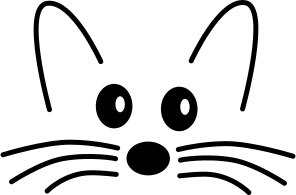
\includegraphics[width=1.4em]{squeak-logo}}}
\iftoshelse{
	\usepackage{marginnote}
		\renewcommand*{\marginfont}{\footnotesize}
	\newcommand{\vartriangleout}{\ifthenelse{\isodd{\thepage}}{\vartriangleright}{\vartriangleleft}}
	\newcommand{\dothisicon}{\fcolorbox{blue!65}{white}{\highlight{$\vartriangleout$}}}
	\newcommand{\dothis}[1]{%
		\noindent\par\noindent
		{\reversemarginpar
			\marginnote{\fcolorbox{blue!65}{white}{\highlight{$\vartriangleout$}}}}
		%\MarginLabel{do this}
		\noindent\emph{#1}
		\nopagebreak}
}{
	\newcommand{\dothisicon}{\raisebox{-.5ex}{
\includegraphics[height=1.2em]{pharo}}}
	\newcommand{\dothis}[1]{%
		\medskip
		\noindent\dothisicon
		\ifx#1\empty\else\quad\emph{#1}\fi
		\par\smallskip\nopagebreak}
}
%===> NEW VERSION <===
% NB: To use this in an individual chapter, you must set:
%\graphicspath{{figures/} {../figures/}}
% at the head of the chapter.  Don't forget the final /
%=============================================================
%:Reader hints (hint)
%
% Indicates a non-obvious consequence 
\newcommand{\hint}[1]{\vspace{1ex}\noindent\fbox{\textsc{Hint}} \emph{#1}}
%=================================================================
% graphics for Morphic handles
\newcommand{\grabHandle}{\raisebox{-0.2ex}{
\includegraphics[width=1em]{blackHandle}}}
\newcommand{\moveHandle}{\raisebox{-0.2ex}{
\includegraphics[width=1em]{moveHandle}}}
\newcommand{\debugHandle}{\raisebox{-0.2ex}{
\includegraphics[width=1em]{debugHandle}}}
%=============================================================
%:Highlighting Important stuff (doublebox)
%
% From Seaside book ...
\newsavebox{\SavedText}
\newlength{\InnerBoxRule}\setlength{\InnerBoxRule}{.75\fboxrule}
\newlength{\OuterBoxRule}\setlength{\OuterBoxRule}{1.5\fboxrule}
\newlength{\BoxSeparation}\setlength{\BoxSeparation}{1.5\fboxrule}
\addtolength{\BoxSeparation}{.5pt}
\newlength{\SaveBoxSep}\setlength{\SaveBoxSep}{2\fboxsep}
%
\newenvironment{doublebox}{\begin{lrbox}{\SavedText}
    \begin{minipage}{.75\textwidth}}
    {\end{minipage}\end{lrbox}\begin{center}
    \setlength{\fboxsep}{\BoxSeparation}\setlength{\fboxrule}{\OuterBoxRule}
    \fbox{\setlength{\fboxsep}{\SaveBoxSep}\setlength{\fboxrule}{\InnerBoxRule}%
      \fbox{\usebox{\SavedText}}}
  \end{center}}
% Use this:
\newcommand{\important}[1]{\begin{doublebox}#1\end{doublebox}}
%=============================================================
%:Section depth
\setcounter{secnumdepth}{2}
%% for this to happen start the file with
%\ifx\wholebook\relax\else
%% $Author$
% $Date$
% $Revision$

% HISTORY:
% 2006-10-31 - Oscar code macros
% ...

%=============================================================
% NB: documentclass must be set in main document.
% Allows book to be generated in multiple formats.
%=============================================================
%:Packages
\usepackage[T1]{fontenc}  %%%%%% really important to get the code directly in the text!
\usepackage{lmodern}
%\usepackage[scaled=0.85]{bookmanx} % needs another scale factor if used with \renewcommand{\sfdefault}{cmbr}
\usepackage{palatino}
\usepackage[scaled=0.85]{helvet}
\usepackage{microtype}
\usepackage{graphicx}
\usepackage{theorem}
\usepackage[english]{babel}
% ON: pdfsync breaks the use of p{width} for tabular columns!
\ifdefined\usepdfsync\usepackage{pdfsync}\fi % Requires texlive 2007
%=============================================================
%:More packages
%Stef should check which ones are used!
%\usepackage{picinpar}
%\usepackage{layout}
%\usepackage{color}
%\usepackage{enum}
%\usepackage{a4wide}
% \usepackage{fancyhdr}
\usepackage{ifthen}
\usepackage{float}
\usepackage{longtable}
\usepackage{makeidx}
\usepackage[nottoc]{tocbibind}
\usepackage{multicol}
\usepackage{booktabs}	% book-style tables
\usepackage{topcapt}	% enables \topcaption
\usepackage{multirow}
\usepackage{tabularx}
%\usepackage[bottom]{footmisc}
\usepackage{xspace}
\usepackage{alltt}
\usepackage{amssymb,textcomp}
\usepackage[usenames,dvipsnames]{color}
%\usepackage{colortbl}
\usepackage[hang]{subfigure}\makeatletter\def\p@subfigure{\thefigure\,}\makeatother
\usepackage{rotating}
\usepackage{enumitem}	% apb: allows more control over tags in enumerations
\usepackage{verbatim}     % for comment environment
\usepackage{varioref}	% for page references that work
\labelformat{footnote}{\thechapter--#1} % to distinguish citations from jurabib
\usepackage{needspace}
\usepackage{isodateo} % enable \isodate
\usepackage[newparttoc]{titlesec}
\usepackage{titletoc}
\usepackage{wrapfig}
\usepackage[
	super,
	citefull=first,
	authorformat={allreversed,and},
	titleformat={commasep,italic}
]{jurabib} % citations as footnotes
\usepackage[
	colorlinks=true,
	linkcolor=black,
	urlcolor=black,
	citecolor=black
]{hyperref}   % should come last
%=============================================================
%:PDF version
\pdfminorversion=3 % Set PDF to 1.3 for Lulu
%=============================================================
%:URL style
\makeatletter
\def\url@leostyle{%
  \@ifundefined{selectfont}{\def\UrlFont{\sf}}{\def\UrlFont{\sffamily}}}
\makeatother
% Now actually use the newly defined style.
\urlstyle{leo}
%=============================================================
%:Booleans
\newboolean{lulu}
\setboolean{lulu}{false}
\newcommand{\ifluluelse}[2]{\ifthenelse{\boolean{lulu}}{#1}{#2}}
%=============================================================
%:Names
\newcommand{\SUnit}{SUnit\xspace}
\newcommand{\sunit}{SUnit\xspace}
\newcommand{\xUnit}{$x$Unit\xspace}
\newcommand{\JUnit}{JUnit\xspace}
\newcommand{\st}{Smalltalk\xspace}
\newcommand{\pharo}{Pharo\xspace} % Use this, not \Pharo
%\newcommand{\sqmap}{SqueakMap\xspace}
\newcommand{\squeak}{Squeak\xspace} % use this, not \Squeak or \sq
\newcommand{\sqsrc}{SqueakSource\xspace}
\newcommand{\sbe}{\url{http://SqueakByExample.org}\xspace}
\newcommand{\pharoweb}{\url{http://pharo-project.org}\xspace}
\newcommand{\pbe}{\url{http://PharoByExample.org}\xspace}
\newcommand{\sba}{\url{http://SquareBracketAssociates.org}\xspace}
\newcommand{\bam}{\lct{Bounc\-ing\-Atoms\-Morph}\xspace}
%=============================================================
%:Markup macros for proof-reading
\usepackage[normalem]{ulem} % for \sout
\usepackage{xcolor}
\newcommand{\ra}{$\rightarrow$}
\newcommand{\ugh}[1]{\textcolor{red}{\uwave{#1}}} % please rephrase
\newcommand{\ins}[1]{\textcolor{blue}{\uline{#1}}} % please insert
\newcommand{\del}[1]{\textcolor{red}{\sout{#1}}} % please delete
\newcommand{\chg}[2]{\textcolor{red}{\sout{#1}}{\ra}\textcolor{blue}{\uline{#2}}} % please change
%=============================================================
%:Editorial comment macros
%\newcommand{\nnbb}[2]{
%    % \fbox{\bfseries\sffamily\scriptsize#1}
%    \fcolorbox{gray}{yellow}{\bfseries\sffamily\scriptsize#1}
%    {\sf\small$\blacktriangleright$\textit{#2}$\blacktriangleleft$}
%   }
\newcommand{\yellowbox}[1]{\fcolorbox{gray}{yellow}{\bfseries\sffamily\scriptsize#1}}
\newcommand{\triangles}[1]{{\sf\small$\blacktriangleright$\textit{#1}$\blacktriangleleft$}}
\newcommand{\nnbb}[2]{\yellowbox{#1} \triangles{#2}}
\newcommand{\fix}{\yellowbox{FIX!}}
\newcommand{\here}{\yellowbox{CONTINUE HERE!}}
% editor macros
\newcommand{\ab}[1]{\nnbb{Andrew}{#1}} % Black
\newcommand{\sd}[1]{\nnbb{St\'{e}f}{#1}} % Ducasse
\newcommand{\md}[1]{\nnbb{Marcus}{#1}} % Denker
\newcommand{\on}[1]{\nnbb{Oscar}{#1}} % Nierstrasz
\newcommand{\damien}[1]{\nnbb{Damien}{#1}} % Pollet
\newcommand{\lr}[1]{\nnbb{Lukas}{#1}} % Renggli
\newcommand{\orla}[1]{\nnbb{Orla}{#1}} % Greevy
\newcommand{\alex}[1]{\nnbb{Alex}{#1}} % Bergel
\newcommand{\alx}[1]{\nnbb{Alex}{#1}} % Bergel
\newcommand{\dr}[1]{\nnbb{David}{#1}} % Roethlisberger
\newcommand{\ja}[1]{\nnbb{Jannik}{#1}} % Laval
\newcommand{\jr}[1]{\nnbb{Jorge}{#1}} % Ressia
\newcommand{\fp}[1]{\nnbb{Fabrizio}{#1}} % Perin
\newcommand{\michael}[1]{\nnbb{Michael}{#1}} % Davies
\newcommand{\ew}[1]{\nnbb{Erwann}{#1}} % Wernli
\newcommand{\mb}[1]{\nnbb{Martial}{#1}} % Boniou
\newcommand{\hw}[1]{\nnbb{Hernan}{#1}} % Wilkinson
%=============================================================
%:Abbreviation macros
\newcommand{\ie}{\emph{i.e.},\xspace}
\newcommand{\eg}{\emph{e.g.},\xspace}
\newcommand{\etc}{etc.\xspace}
%=============================================================
%:Cross reference macros
\newcommand{\charef}[1]{Chapter~\ref{cha:#1}\xspace}
\newcommand{\secref}[1]{Section~\ref{sec:#1}\xspace}
\newcommand{\figref}[1]{Figure~\ref{fig:#1}\xspace}
\newcommand{\Figref}[1]{Figure~\ref{fig:#1}\xspace}
\newcommand{\appref}[1]{Appendix~\ref{app:#1}\xspace}
\newcommand{\tabref}[1]{Table~\ref{tab:#1}\xspace}
\newcommand{\faqref}[1]{FAQ~\ref{faq:#1}, p.~\pageref{faq:#1}\xspace}
% APB: I removed trailing \xspace commands from these macros because
% \xspace mostly doesn't work.  If you want a space after your
% references, type one!
% ON: xspace has always worked just fine for me!  Please leave them in.
%
\newcommand{\ruleref}[1]{\ref{rule:#1}\xspace}
%
\newcommand{\egref}[1]{example~\ref{eg:#1}\xspace}
\newcommand{\Egref}[1]{Example~\ref{eg:#1}\xspace}
%
\newcommand{\scrref}[1]{script~\ref{scr:#1}\xspace}
\newcommand{\Scrref}[1]{Script~\ref{scr:#1}\xspace}
\newcommand{\tscrref}[1]{the script~\ref{scr:#1}\xspace}
\newcommand{\Tscrref}[1]{The script~\ref{scr:#1}\xspace}
%
\newcommand{\mthref}[1]{method~\ref{mth:#1}\xspace}
\newcommand{\mthsref}[1]{methods~\ref{mth:#1}\xspace}
\newcommand{\Mthref}[1]{Method~\ref{mth:#1}\xspace}
\newcommand{\tmthref}[1]{the method~\ref{mth:#1}\xspace}
\newcommand{\Tmthref}[1]{The method~\ref{mth:#1}\xspace}
%
\newcommand{\clsref}[1]{class~\ref{cls:#1}\xspace}
\newcommand{\tclsref}[1]{the class~\ref{cls:#1}\xspace}
\newcommand{\Tclsref}[1]{The class~\ref{cls:#1}\xspace}

\newcommand{\chalabel}[1]{\label{cha:#1}}
\newcommand{\seclabel}[1]{\label{sec:#1}}
\newcommand{\figlabel}[1]{\label{fig:#1}}
\newcommand{\tablabel}[1]{\label{tab:#1}}
\newcommand{\rulelabel}[1]{\label{rule:#1}}
\newcommand{\eglabel}[1]{\label{eg:#1}}
\newcommand{\scrlabel}[1]{\label{scr:#1}}
\newcommand{\mthlabel}[1]{\label{mth:#1}}
\newcommand{\clslabel}[1]{\label{cls:#1}}
\newcommand{\faqlabel}[1]{\label{faq:#1}}
%=============================================================
%:Menu item macro
% for menu items, so we can change our minds on how to print them! (apb)
\definecolor{lightgray}{gray}{0.89}
\newcommand{\menu}[1]{{%
	\setlength{\fboxsep}{0pt}%
	\colorbox{lightgray}{{{\upshape\sffamily\strut \,#1\,}}}}}
\newcommand{\link}[1]{{%
	\fontfamily{lmr}\selectfont
 	\upshape{\sffamily \underline{#1}}}}
% For submenu items:
\newcommand{\go}{\,$\triangleright$\,}
% \newcommand{\go}{\,$\blacktriangleright$\,}
% For keyboard shortcuts:
%\newcommand{\short}[1]{\mbox{$\langle${\sc CMD}$\rangle$-#1}\xspace}
\newcommand{\short}[1]{\mbox{{\sc cmd}\hspace{0.08em}--\hspace{0.09em}#1}\xspace}
% For buttons:
\newcommand{\button}[1]{{%
	\setlength{\fboxsep}{0pt}%
	\fbox{{\upshape\sffamily\strut \,#1\,}}}}
% NB: The button macro does not work within captions -- incompatible with xcolor package :-(
\newcommand{\toolsflap}{\textit{Tools} flap\xspace}
%=============================================================
%:Mouse clicks
\newcommand{\click}{click\xspace} % RED
\newcommand{\actclick}{action-click\xspace} % YELLOW
\newcommand{\metaclick}{meta-click\xspace} % BLUE
\newcommand{\Click}{Click\xspace} % RED
\newcommand{\Actclick}{Action-click\xspace} % YELLOW
\newcommand{\Metaclick}{Meta-click\xspace} % BLUE
%=============================================================
%:ToSh macros
\newboolean{tosh}
\setboolean{tosh}{false}
\newcommand{\iftoshelse}[2]{\ifthenelse{\boolean{tosh}}{#1}{#2}}
%=============================================================
%:ToSh colors
%\newcommand{\highlightcolor}{\color{blue!65}}
%\newcommand{\boxcolor}{\color{gray!25}}
\newcommand{\highlight}[1]{\textcolor{blue!65}{#1}}
%\newcommand{\codecolor}{\color{blue!65}}
%%\setlength{\fboxrule}{2pt}
%\newcommand{\asPict}[1]{%
%	{\Large\highlight{#1}}}
%=============================================================
%:Reader cues (do this)
%
% Indicate something the reader should try out.
% \newcommand{\dothisicon}{\raisebox{-.5ex}{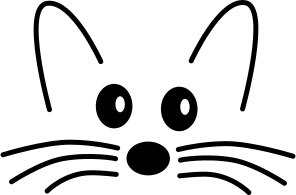
\includegraphics[width=1.4em]{squeak-logo}}}
\iftoshelse{
	\usepackage{marginnote}
		\renewcommand*{\marginfont}{\footnotesize}
	\newcommand{\vartriangleout}{\ifthenelse{\isodd{\thepage}}{\vartriangleright}{\vartriangleleft}}
	\newcommand{\dothisicon}{\fcolorbox{blue!65}{white}{\highlight{$\vartriangleout$}}}
	\newcommand{\dothis}[1]{%
		\noindent\par\noindent
		{\reversemarginpar
			\marginnote{\fcolorbox{blue!65}{white}{\highlight{$\vartriangleout$}}}}
		%\MarginLabel{do this}
		\noindent\emph{#1}
		\nopagebreak}
}{
	\newcommand{\dothisicon}{\raisebox{-.5ex}{
\includegraphics[height=1.2em]{pharo}}}
	\newcommand{\dothis}[1]{%
		\medskip
		\noindent\dothisicon
		\ifx#1\empty\else\quad\emph{#1}\fi
		\par\smallskip\nopagebreak}
}
%===> NEW VERSION <===
% NB: To use this in an individual chapter, you must set:
%\graphicspath{{figures/} {../figures/}}
% at the head of the chapter.  Don't forget the final /
%=============================================================
%:Reader hints (hint)
%
% Indicates a non-obvious consequence 
\newcommand{\hint}[1]{\vspace{1ex}\noindent\fbox{\textsc{Hint}} \emph{#1}}
%=================================================================
% graphics for Morphic handles
\newcommand{\grabHandle}{\raisebox{-0.2ex}{
\includegraphics[width=1em]{blackHandle}}}
\newcommand{\moveHandle}{\raisebox{-0.2ex}{
\includegraphics[width=1em]{moveHandle}}}
\newcommand{\debugHandle}{\raisebox{-0.2ex}{
\includegraphics[width=1em]{debugHandle}}}
%=============================================================
%:Highlighting Important stuff (doublebox)
%
% From Seaside book ...
\newsavebox{\SavedText}
\newlength{\InnerBoxRule}\setlength{\InnerBoxRule}{.75\fboxrule}
\newlength{\OuterBoxRule}\setlength{\OuterBoxRule}{1.5\fboxrule}
\newlength{\BoxSeparation}\setlength{\BoxSeparation}{1.5\fboxrule}
\addtolength{\BoxSeparation}{.5pt}
\newlength{\SaveBoxSep}\setlength{\SaveBoxSep}{2\fboxsep}
%
\newenvironment{doublebox}{\begin{lrbox}{\SavedText}
    \begin{minipage}{.75\textwidth}}
    {\end{minipage}\end{lrbox}\begin{center}
    \setlength{\fboxsep}{\BoxSeparation}\setlength{\fboxrule}{\OuterBoxRule}
    \fbox{\setlength{\fboxsep}{\SaveBoxSep}\setlength{\fboxrule}{\InnerBoxRule}%
      \fbox{\usebox{\SavedText}}}
  \end{center}}
% Use this:
\newcommand{\important}[1]{\begin{doublebox}#1\end{doublebox}}
%=============================================================
%:Section depth
\setcounter{secnumdepth}{2}
%% for this to happen start the file with
%\ifx\wholebook\relax\else
%% $Author$
% $Date$
% $Revision$

% HISTORY:
% 2006-10-31 - Oscar code macros
% ...

%=============================================================
% NB: documentclass must be set in main document.
% Allows book to be generated in multiple formats.
%=============================================================
%:Packages
\usepackage[T1]{fontenc}  %%%%%% really important to get the code directly in the text!
\usepackage{lmodern}
%\usepackage[scaled=0.85]{bookmanx} % needs another scale factor if used with \renewcommand{\sfdefault}{cmbr}
\usepackage{palatino}
\usepackage[scaled=0.85]{helvet}
\usepackage{microtype}
\usepackage{graphicx}
\usepackage{theorem}
\usepackage[english]{babel}
% ON: pdfsync breaks the use of p{width} for tabular columns!
\ifdefined\usepdfsync\usepackage{pdfsync}\fi % Requires texlive 2007
%=============================================================
%:More packages
%Stef should check which ones are used!
%\usepackage{picinpar}
%\usepackage{layout}
%\usepackage{color}
%\usepackage{enum}
%\usepackage{a4wide}
% \usepackage{fancyhdr}
\usepackage{ifthen}
\usepackage{float}
\usepackage{longtable}
\usepackage{makeidx}
\usepackage[nottoc]{tocbibind}
\usepackage{multicol}
\usepackage{booktabs}	% book-style tables
\usepackage{topcapt}	% enables \topcaption
\usepackage{multirow}
\usepackage{tabularx}
%\usepackage[bottom]{footmisc}
\usepackage{xspace}
\usepackage{alltt}
\usepackage{amssymb,textcomp}
\usepackage[usenames,dvipsnames]{color}
%\usepackage{colortbl}
\usepackage[hang]{subfigure}\makeatletter\def\p@subfigure{\thefigure\,}\makeatother
\usepackage{rotating}
\usepackage{enumitem}	% apb: allows more control over tags in enumerations
\usepackage{verbatim}     % for comment environment
\usepackage{varioref}	% for page references that work
\labelformat{footnote}{\thechapter--#1} % to distinguish citations from jurabib
\usepackage{needspace}
\usepackage{isodateo} % enable \isodate
\usepackage[newparttoc]{titlesec}
\usepackage{titletoc}
\usepackage{wrapfig}
\usepackage[
	super,
	citefull=first,
	authorformat={allreversed,and},
	titleformat={commasep,italic}
]{jurabib} % citations as footnotes
\usepackage[
	colorlinks=true,
	linkcolor=black,
	urlcolor=black,
	citecolor=black
]{hyperref}   % should come last
%=============================================================
%:PDF version
\pdfminorversion=3 % Set PDF to 1.3 for Lulu
%=============================================================
%:URL style
\makeatletter
\def\url@leostyle{%
  \@ifundefined{selectfont}{\def\UrlFont{\sf}}{\def\UrlFont{\sffamily}}}
\makeatother
% Now actually use the newly defined style.
\urlstyle{leo}
%=============================================================
%:Booleans
\newboolean{lulu}
\setboolean{lulu}{false}
\newcommand{\ifluluelse}[2]{\ifthenelse{\boolean{lulu}}{#1}{#2}}
%=============================================================
%:Names
\newcommand{\SUnit}{SUnit\xspace}
\newcommand{\sunit}{SUnit\xspace}
\newcommand{\xUnit}{$x$Unit\xspace}
\newcommand{\JUnit}{JUnit\xspace}
\newcommand{\st}{Smalltalk\xspace}
\newcommand{\pharo}{Pharo\xspace} % Use this, not \Pharo
%\newcommand{\sqmap}{SqueakMap\xspace}
\newcommand{\squeak}{Squeak\xspace} % use this, not \Squeak or \sq
\newcommand{\sqsrc}{SqueakSource\xspace}
\newcommand{\sbe}{\url{http://SqueakByExample.org}\xspace}
\newcommand{\pharoweb}{\url{http://pharo-project.org}\xspace}
\newcommand{\pbe}{\url{http://PharoByExample.org}\xspace}
\newcommand{\sba}{\url{http://SquareBracketAssociates.org}\xspace}
\newcommand{\bam}{\lct{Bounc\-ing\-Atoms\-Morph}\xspace}
%=============================================================
%:Markup macros for proof-reading
\usepackage[normalem]{ulem} % for \sout
\usepackage{xcolor}
\newcommand{\ra}{$\rightarrow$}
\newcommand{\ugh}[1]{\textcolor{red}{\uwave{#1}}} % please rephrase
\newcommand{\ins}[1]{\textcolor{blue}{\uline{#1}}} % please insert
\newcommand{\del}[1]{\textcolor{red}{\sout{#1}}} % please delete
\newcommand{\chg}[2]{\textcolor{red}{\sout{#1}}{\ra}\textcolor{blue}{\uline{#2}}} % please change
%=============================================================
%:Editorial comment macros
%\newcommand{\nnbb}[2]{
%    % \fbox{\bfseries\sffamily\scriptsize#1}
%    \fcolorbox{gray}{yellow}{\bfseries\sffamily\scriptsize#1}
%    {\sf\small$\blacktriangleright$\textit{#2}$\blacktriangleleft$}
%   }
\newcommand{\yellowbox}[1]{\fcolorbox{gray}{yellow}{\bfseries\sffamily\scriptsize#1}}
\newcommand{\triangles}[1]{{\sf\small$\blacktriangleright$\textit{#1}$\blacktriangleleft$}}
\newcommand{\nnbb}[2]{\yellowbox{#1} \triangles{#2}}
\newcommand{\fix}{\yellowbox{FIX!}}
\newcommand{\here}{\yellowbox{CONTINUE HERE!}}
% editor macros
\newcommand{\ab}[1]{\nnbb{Andrew}{#1}} % Black
\newcommand{\sd}[1]{\nnbb{St\'{e}f}{#1}} % Ducasse
\newcommand{\md}[1]{\nnbb{Marcus}{#1}} % Denker
\newcommand{\on}[1]{\nnbb{Oscar}{#1}} % Nierstrasz
\newcommand{\damien}[1]{\nnbb{Damien}{#1}} % Pollet
\newcommand{\lr}[1]{\nnbb{Lukas}{#1}} % Renggli
\newcommand{\orla}[1]{\nnbb{Orla}{#1}} % Greevy
\newcommand{\alex}[1]{\nnbb{Alex}{#1}} % Bergel
\newcommand{\alx}[1]{\nnbb{Alex}{#1}} % Bergel
\newcommand{\dr}[1]{\nnbb{David}{#1}} % Roethlisberger
\newcommand{\ja}[1]{\nnbb{Jannik}{#1}} % Laval
\newcommand{\jr}[1]{\nnbb{Jorge}{#1}} % Ressia
\newcommand{\fp}[1]{\nnbb{Fabrizio}{#1}} % Perin
\newcommand{\michael}[1]{\nnbb{Michael}{#1}} % Davies
\newcommand{\ew}[1]{\nnbb{Erwann}{#1}} % Wernli
\newcommand{\mb}[1]{\nnbb{Martial}{#1}} % Boniou
\newcommand{\hw}[1]{\nnbb{Hernan}{#1}} % Wilkinson
%=============================================================
%:Abbreviation macros
\newcommand{\ie}{\emph{i.e.},\xspace}
\newcommand{\eg}{\emph{e.g.},\xspace}
\newcommand{\etc}{etc.\xspace}
%=============================================================
%:Cross reference macros
\newcommand{\charef}[1]{Chapter~\ref{cha:#1}\xspace}
\newcommand{\secref}[1]{Section~\ref{sec:#1}\xspace}
\newcommand{\figref}[1]{Figure~\ref{fig:#1}\xspace}
\newcommand{\Figref}[1]{Figure~\ref{fig:#1}\xspace}
\newcommand{\appref}[1]{Appendix~\ref{app:#1}\xspace}
\newcommand{\tabref}[1]{Table~\ref{tab:#1}\xspace}
\newcommand{\faqref}[1]{FAQ~\ref{faq:#1}, p.~\pageref{faq:#1}\xspace}
% APB: I removed trailing \xspace commands from these macros because
% \xspace mostly doesn't work.  If you want a space after your
% references, type one!
% ON: xspace has always worked just fine for me!  Please leave them in.
%
\newcommand{\ruleref}[1]{\ref{rule:#1}\xspace}
%
\newcommand{\egref}[1]{example~\ref{eg:#1}\xspace}
\newcommand{\Egref}[1]{Example~\ref{eg:#1}\xspace}
%
\newcommand{\scrref}[1]{script~\ref{scr:#1}\xspace}
\newcommand{\Scrref}[1]{Script~\ref{scr:#1}\xspace}
\newcommand{\tscrref}[1]{the script~\ref{scr:#1}\xspace}
\newcommand{\Tscrref}[1]{The script~\ref{scr:#1}\xspace}
%
\newcommand{\mthref}[1]{method~\ref{mth:#1}\xspace}
\newcommand{\mthsref}[1]{methods~\ref{mth:#1}\xspace}
\newcommand{\Mthref}[1]{Method~\ref{mth:#1}\xspace}
\newcommand{\tmthref}[1]{the method~\ref{mth:#1}\xspace}
\newcommand{\Tmthref}[1]{The method~\ref{mth:#1}\xspace}
%
\newcommand{\clsref}[1]{class~\ref{cls:#1}\xspace}
\newcommand{\tclsref}[1]{the class~\ref{cls:#1}\xspace}
\newcommand{\Tclsref}[1]{The class~\ref{cls:#1}\xspace}

\newcommand{\chalabel}[1]{\label{cha:#1}}
\newcommand{\seclabel}[1]{\label{sec:#1}}
\newcommand{\figlabel}[1]{\label{fig:#1}}
\newcommand{\tablabel}[1]{\label{tab:#1}}
\newcommand{\rulelabel}[1]{\label{rule:#1}}
\newcommand{\eglabel}[1]{\label{eg:#1}}
\newcommand{\scrlabel}[1]{\label{scr:#1}}
\newcommand{\mthlabel}[1]{\label{mth:#1}}
\newcommand{\clslabel}[1]{\label{cls:#1}}
\newcommand{\faqlabel}[1]{\label{faq:#1}}
%=============================================================
%:Menu item macro
% for menu items, so we can change our minds on how to print them! (apb)
\definecolor{lightgray}{gray}{0.89}
\newcommand{\menu}[1]{{%
	\setlength{\fboxsep}{0pt}%
	\colorbox{lightgray}{{{\upshape\sffamily\strut \,#1\,}}}}}
\newcommand{\link}[1]{{%
	\fontfamily{lmr}\selectfont
 	\upshape{\sffamily \underline{#1}}}}
% For submenu items:
\newcommand{\go}{\,$\triangleright$\,}
% \newcommand{\go}{\,$\blacktriangleright$\,}
% For keyboard shortcuts:
%\newcommand{\short}[1]{\mbox{$\langle${\sc CMD}$\rangle$-#1}\xspace}
\newcommand{\short}[1]{\mbox{{\sc cmd}\hspace{0.08em}--\hspace{0.09em}#1}\xspace}
% For buttons:
\newcommand{\button}[1]{{%
	\setlength{\fboxsep}{0pt}%
	\fbox{{\upshape\sffamily\strut \,#1\,}}}}
% NB: The button macro does not work within captions -- incompatible with xcolor package :-(
\newcommand{\toolsflap}{\textit{Tools} flap\xspace}
%=============================================================
%:Mouse clicks
\newcommand{\click}{click\xspace} % RED
\newcommand{\actclick}{action-click\xspace} % YELLOW
\newcommand{\metaclick}{meta-click\xspace} % BLUE
\newcommand{\Click}{Click\xspace} % RED
\newcommand{\Actclick}{Action-click\xspace} % YELLOW
\newcommand{\Metaclick}{Meta-click\xspace} % BLUE
%=============================================================
%:ToSh macros
\newboolean{tosh}
\setboolean{tosh}{false}
\newcommand{\iftoshelse}[2]{\ifthenelse{\boolean{tosh}}{#1}{#2}}
%=============================================================
%:ToSh colors
%\newcommand{\highlightcolor}{\color{blue!65}}
%\newcommand{\boxcolor}{\color{gray!25}}
\newcommand{\highlight}[1]{\textcolor{blue!65}{#1}}
%\newcommand{\codecolor}{\color{blue!65}}
%%\setlength{\fboxrule}{2pt}
%\newcommand{\asPict}[1]{%
%	{\Large\highlight{#1}}}
%=============================================================
%:Reader cues (do this)
%
% Indicate something the reader should try out.
% \newcommand{\dothisicon}{\raisebox{-.5ex}{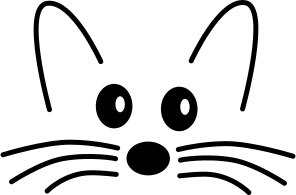
\includegraphics[width=1.4em]{squeak-logo}}}
\iftoshelse{
	\usepackage{marginnote}
		\renewcommand*{\marginfont}{\footnotesize}
	\newcommand{\vartriangleout}{\ifthenelse{\isodd{\thepage}}{\vartriangleright}{\vartriangleleft}}
	\newcommand{\dothisicon}{\fcolorbox{blue!65}{white}{\highlight{$\vartriangleout$}}}
	\newcommand{\dothis}[1]{%
		\noindent\par\noindent
		{\reversemarginpar
			\marginnote{\fcolorbox{blue!65}{white}{\highlight{$\vartriangleout$}}}}
		%\MarginLabel{do this}
		\noindent\emph{#1}
		\nopagebreak}
}{
	\newcommand{\dothisicon}{\raisebox{-.5ex}{
\includegraphics[height=1.2em]{pharo}}}
	\newcommand{\dothis}[1]{%
		\medskip
		\noindent\dothisicon
		\ifx#1\empty\else\quad\emph{#1}\fi
		\par\smallskip\nopagebreak}
}
%===> NEW VERSION <===
% NB: To use this in an individual chapter, you must set:
%\graphicspath{{figures/} {../figures/}}
% at the head of the chapter.  Don't forget the final /
%=============================================================
%:Reader hints (hint)
%
% Indicates a non-obvious consequence 
\newcommand{\hint}[1]{\vspace{1ex}\noindent\fbox{\textsc{Hint}} \emph{#1}}
%=================================================================
% graphics for Morphic handles
\newcommand{\grabHandle}{\raisebox{-0.2ex}{
\includegraphics[width=1em]{blackHandle}}}
\newcommand{\moveHandle}{\raisebox{-0.2ex}{
\includegraphics[width=1em]{moveHandle}}}
\newcommand{\debugHandle}{\raisebox{-0.2ex}{
\includegraphics[width=1em]{debugHandle}}}
%=============================================================
%:Highlighting Important stuff (doublebox)
%
% From Seaside book ...
\newsavebox{\SavedText}
\newlength{\InnerBoxRule}\setlength{\InnerBoxRule}{.75\fboxrule}
\newlength{\OuterBoxRule}\setlength{\OuterBoxRule}{1.5\fboxrule}
\newlength{\BoxSeparation}\setlength{\BoxSeparation}{1.5\fboxrule}
\addtolength{\BoxSeparation}{.5pt}
\newlength{\SaveBoxSep}\setlength{\SaveBoxSep}{2\fboxsep}
%
\newenvironment{doublebox}{\begin{lrbox}{\SavedText}
    \begin{minipage}{.75\textwidth}}
    {\end{minipage}\end{lrbox}\begin{center}
    \setlength{\fboxsep}{\BoxSeparation}\setlength{\fboxrule}{\OuterBoxRule}
    \fbox{\setlength{\fboxsep}{\SaveBoxSep}\setlength{\fboxrule}{\InnerBoxRule}%
      \fbox{\usebox{\SavedText}}}
  \end{center}}
% Use this:
\newcommand{\important}[1]{\begin{doublebox}#1\end{doublebox}}
%=============================================================
%:Section depth
\setcounter{secnumdepth}{2}
%% for this to happen start the file with
%\ifx\wholebook\relax\else
%\input{../common.tex}
%\begin{document}
%\fi
% and terminate by
% \ifx\wholebook\relax\else\end{document}\fi

\DeclareGraphicsExtensions{.pdf, .jpg, .png}
%=============================================================
%:PDF setup
\hypersetup{
%   a4paper,
%   pdfstartview=FitV,
%   colorlinks,
%   linkcolor=darkblue,
%   citecolor=darkblue,
   pdftitle={Pharo by Example},
   pdfauthor={Andrew P. Black, St\'ephane Ducasse,	Oscar Nierstrasz,
Damien Pollet},
   pdfkeywords={Smalltalk, Squeak, Object-Oriented Programming, OOP},
   pdfsubject={Computer Science}
}
%=============================================================
%:Page layout and appearance
%
% \renewcommand{\headrulewidth}{0pt}
\renewcommand{\chaptermark}[1]{\markboth{#1}{}}
\renewcommand{\sectionmark}[1]{\markright{\thesection\ #1}}
\renewpagestyle{plain}[\small\itshape]{%
	\setheadrule{0pt}%
	\sethead[][][]{}{}{}%
	\setfoot[][][]{}{}{}}
\renewpagestyle{headings}[\small\itshape]{%
	\setheadrule{0pt}%
	\setmarks{chapter}{section}%
	\sethead[\thepage][][\chaptertitle]{\sectiontitle}{}{\thepage}%
	\setfoot[][][]{}{}{}}
%=============================================================
%:Title section setup and TOC numbering depth
\setcounter{secnumdepth}{1}
\setcounter{tocdepth}{1}
\titleformat{\part}[display]{\centering}{\huge\partname\ \thepart}{1em}{\Huge\textbf}[]
\titleformat{\chapter}[display]{}{\huge\chaptertitlename\ \thechapter}{1em}{\Huge\raggedright\textbf}[]
\titlecontents{part}[3pc]{%
		\pagebreak[2]\addvspace{1em plus.4em minus.2em}%
		\leavevmode\large\bfseries}
	{\contentslabel{3pc}}{\hspace*{-3pc}}
	{}[\nopagebreak]
\titlecontents{chapter}[3pc]{%
		\pagebreak[0]\addvspace{1em plus.2em minus.2em}%
		\leavevmode\bfseries}
	{\contentslabel{3pc}}{}
	{\hfill\contentspage}[\nopagebreak]
\dottedcontents{section}[3pc]{}{3pc}{1pc}
\dottedcontents{subsection}[3pc]{}{0pc}{1pc}
% \dottedcontents{subsection}[4.5em]{}{0pt}{1pc}
% Make \cleardoublepage insert really blank pages http://www.tex.ac.uk/cgi-bin/texfaq2html?label=reallyblank
\let\origdoublepage\cleardoublepage
\newcommand{\clearemptydoublepage}{%
  \clearpage
  {\pagestyle{empty}\origdoublepage}}
\let\cleardoublepage\clearemptydoublepage % see http://www.tex.ac.uk/cgi-bin/texfaq2html?label=patch
%=============================================================
%:FAQ macros (for FAQ chapter)
\newtheorem{faq}{FAQ}
\newcommand{\answer}{\paragraph{Answer}\ }
%=============================================================
%:Listings package configuration
% \newcommand{\caret}{\makebox{\raisebox{0.4ex}{\footnotesize{$\wedge$}}}}
\newcommand{\caret}{\^\,}
\newcommand{\escape}{{\sf \textbackslash}}
\definecolor{source}{gray}{0.95}
\usepackage{listings}
\lstdefinelanguage{Smalltalk}{
%  morekeywords={self,super,true,false,nil,thisContext}, % This is overkill
  morestring=[d]',
  morecomment=[s]{"}{"},
  alsoletter={\#:},
  escapechar={!},
  literate=
    {BANG}{!}1
    {CARET}{\^}1
    {UNDERSCORE}{\_}1
    {\\st}{Smalltalk}9 % convenience -- in case \st occurs in code
    % {'}{{\textquotesingle}}1 % replaced by upquote=true in \lstset
    {_}{{$\leftarrow$}}1
    {>>>}{{\sep}}1
    {^}{{$\uparrow$}}1
    {~}{{$\sim$}}1
    {-}{{\textminus}}1 %{-}{\hspace{-0.13em}}{-}}1  % the goal is to make - the same width as +
    % {+}{\sf+}1 %{\raisebox{0.08ex}{+}}}1      % and to raise + off the baseline to match -
    {-->}{{\quad$\longrightarrow$\quad}}3
	, % Don't forget the comma at the end!
  tabsize=4
}[keywords,comments,strings]

\lstset{language=Smalltalk,
	basicstyle=\sffamily,
	keywordstyle=\color{black}\bfseries,
	% stringstyle=\ttfamily, % Ugly! do we really want this? -- on
	mathescape=true,
	showstringspaces=false,
	keepspaces=true,
	breaklines=true,
	breakautoindent=true,
	backgroundcolor=\color{source},
	lineskip={-1pt}, % Ugly hack
	upquote=true, % straight quote; requires textcomp package
	columns=fullflexible} % no fixed width fonts
% In-line code (literal)
% Normally use this for all in-line code:
\newcommand{\ct}{\lstinline[mathescape=false,backgroundcolor=\color{white},basicstyle={\sffamily\upshape}]}
% apb 2007.8.28 added the \upshape declaration to avoid getting italicized code in \dothis{ } sections.
% In-line code (latex enabled)
% Use this only in special situations where \ct does not work
% (within section headings ...):
\newcommand{\lct}[1]{{\textsf{\textup{#1}}}}
% Use these for system categories and protocols:
\newcommand{\scat}[1]{\emph{\textsf{#1}}\xspace}
\newcommand{\pkg}[1]{\emph{\textsf{#1}}\xspace}
\newcommand{\prot}[1]{\emph{\textsf{#1}}\xspace}
% Code environments
% NB: the arg is for tests
% Only code and example environments may be tests
\lstnewenvironment{code}[1]{%
	\lstset{%
		% frame=lines,
		frame=single,
		framerule=0pt,
		mathescape=false
	}
}{}
\def\ignoredollar#1{}
%=============================================================
%:Code environments (method, script ...)
% NB: the third arg is for tests
% Only code and example environments may be tests
\lstnewenvironment{example}[3][defaultlabel]{%
	\renewcommand{\lstlistingname}{Example}%
	\lstset{
		% frame=lines,
		frame=single,
		framerule=0pt,
		mathescape=false,
		caption={\emph{#2}},
		label={eg:#1}
	}
}{}
\lstnewenvironment{script}[2][defaultlabel]{%
\renewcommand{\lstlistingname}{Script}%
	\lstset{
		% frame=lines,
		frame=single,
		framerule=0pt,
		mathescape=false,
		name={Script},
		caption={\emph{#2}},
		label={scr:#1}
	}
}{}
\lstnewenvironment{method}[2][defaultlabel]{%
	\renewcommand{\lstlistingname}{Method}%
	\lstset{
		% frame=lines,
		frame=single,
		framerule=0pt,
		mathescape=false,
		name={Method},
		caption={\emph{#2}},
		label={mth:#1}
	}
}{}
\lstnewenvironment{methods}[2][defaultlabel]{% just for multiple methods at once
	\renewcommand{\lstlistingname}{Methods}%
	\lstset{
		% frame=lines,
		frame=single,
		framerule=0pt,
		mathescape=false,
		name={Method},
		caption={\emph{#2}},
		label={mth:#1}
	}
}{}
\lstnewenvironment{numMethod}[2][defaultlabel]{%
	\renewcommand{\lstlistingname}{Method}%
	\lstset{
		numbers=left,
		numberstyle={\tiny\sffamily},
		% frame=lines,
		frame=single,
		framerule=0pt,
		mathescape=false,
		name={Method},
		caption={\emph{#2}},
		label={mth:#1}
	}
}{}
\lstnewenvironment{classdef}[2][defaultlabel]{%
	\renewcommand{\lstlistingname}{Class}%
	\lstset{
		% frame=lines,
		frame=single,
		framerule=0pt,
		mathescape=false,
		name={Class},
		caption={\emph{#2}},
		label={cls:#1}
	}
}{}
%=============================================================
%:Reserving space
% Usually need one more line than the actual lines of code
\newcommand{\needlines}[1]{\Needspace{#1\baselineskip}}
%=============================================================
%:Indexing macros
% Macros ending with "ind" generate text as well as an index entry
% Macros ending with "index" *only* generate an index entry
\newcommand{\ind}[1]{\index{#1}#1\xspace} % plain text
\newcommand{\subind}[2]{\index{#1!#2}#2\xspace} % show #2, subindex under #1
\newcommand{\emphind}[1]{\index{#1}\emph{#1}\xspace} % emph #1
\newcommand{\emphsubind}[2]{\index{#1!#2}\emph{#2}\xspace} % show emph #2, subindex inder #1
\newcommand{\scatind}[1]{\index{#1@\textsf{#1} (category)}\scat{#1}} % category
\newcommand{\pkgind}[1]{\index{#1@\textsf{#1} (package)}\pkg{#1}} % package
\newcommand{\protind}[1]{\index{#1@\textsf{#1} (protocol)}\prot{#1}} % protocol
\newcommand{\clsind}[1]{\index{#1@\textsf{#1} (class)}\ct{#1}\xspace}
% \newcommand{\clsind}[1]{\index{#1!\#@(class)}\ct{#1}\xspace} % class
\newcommand{\clsindplural}[1]{\index{#1!\#@(class)}\ct{#1}s\xspace} % class
\newcommand{\cvind}[1]{\index{#1@\textsf{#1} (class variable)}\ct{#1}\xspace} % class var
\newcommand{\glbind}[1]{\index{#1@\textsf{#1} (global)}\ct{#1}\xspace} % global
\newcommand{\patind}[1]{\index{#1@#1 (pattern)}\ct{#1}\xspace} % pattern
\newcommand{\pvind}[1]{\index{#1@\textsf{#1} (pseudo variable)}\ct{#1}\xspace} % pseudo var
\newcommand{\clsmthind}[2]{\index{#1!#2@\ct{#2}}\ct{#1>>>#2}\xspace} % class + method name
\newcommand{\mthind}[2]{\index{#1!#2@\ct{#2}}\ct{#2}\xspace} % show method name only
\newcommand{\lmthind}[2]{\index{#1!#2@\ct{#2}}\lct{#2}\xspace} % show method name only
\newcommand{\cmind}[2]{\index{#1!#2@\ct{#2}}\ct{#1>>>#2}\xspace} % show class>>method
\newcommand{\lcmind}[2]{\index{#1!#2@\ct{#2}}\lct{#1>>>#2}\xspace} % show class>>method
\newcommand{\toolsflapind}{\index{Tools flap}\toolsflap} % index tools flap
% The following only generate an index entry:
% \newcommand{\clsindex}[1]{\index{#1@\textsf{#1} (class)}}
\newcommand{\clsindex}[1]{\index{#1!\#@(class)}} % class
\newcommand{\mthindex}[2]{\index{#1!#2@\ct{#2}}} % method
\newcommand{\cmindex}[2]{\index{#1!#2@\ct{#2}}} % class>>method
\newcommand{\cvindex}[1]{\index{#1@\textsf{#1} (class variable)}} % class var
\newcommand{\glbindex}[1]{\index{#1@\textsf{#1} (global)}}% global
\newcommand{\pvindex}[1]{\index{#1@\textsf{#1} (pseudo variable)}}% pseudo var
\newcommand{\seeindex}[2]{\index{#1|see{#2}}} % #1, see #2
\newcommand{\scatindex}[1]{\index{#1@\textsf{#1} (category)}} % category
\newcommand{\pkgindex}[1]{\index{#1@\textsf{#1} (package)}} % package
\newcommand{\protindex}[1]{\index{#1@\textsf{#1} (protocol)}} % protocol
% How can we have the main entry page numbers in bold yet not break the hyperlink?
\newcommand{\boldidx}[1]{{\bf #1}} % breaks hyperlink
%\newcommand{\indmain}[1]{\index{#1|boldidx}#1\xspace} % plain text, main entry
%\newcommand{\emphsubindmain}[2]{\index{#1!#2|boldidx}\emph{#2}\xspace} % subindex, main entry
%\newcommand{\subindmain}[2]{\index{#1!#2|boldidx}#2\xspace} % subindex, main entry
%\newcommand{\clsindmain}[1]{\index{#1@\textsf{#1} (class)|boldidx}\ct{#1}\xspace}
%\newcommand{\clsindmain}[1]{\index{#1!\#@(class)|boldidx}\ct{#1}\xspace} % class main
%\newcommand{\indexmain}[1]{\index{#1|boldidx}} % main index entry only
\newcommand{\indmain}[1]{\index{#1}#1\xspace} % The main index entry for this item
\newcommand{\emphsubindmain}[2]{\index{#1!#2}\emph{#2}\xspace} % subindex, main entry
\newcommand{\subindmain}[2]{\index{#1!#2}#2\xspace} % subindex, main entry
%\newcommand{\clsindmain}[1]{\index{#1@\textsf{#1} (class)}\ct{#1}\xspace}
\newcommand{\clsindmain}[1]{\index{#1!\#@(class)}\ct{#1}\xspace} % class main
\newcommand{\clsindexmain}[1]{\index{#1!\#@(class)}} % class main index only
\newcommand{\indexmain}[1]{\index{#1}} 
%=============================================================
%:Code macros
% some constants
\newcommand{\codesize}{\small}
\newcommand{\codefont}{\sffamily}
%\newcommand{\cat}[1]{\textit{In category #1}}%%To remove later
\newlength{\scriptindent}
\setlength{\scriptindent}{.3cm}
%% Method presentation constants
\newlength{\methodindent}
\newlength{\methodwordlength}
\newlength{\aftermethod}
\setlength{\methodindent}{0.2cm}
\settowidth{\methodwordlength}{\ M\'ethode\ }
%=============================================================
%:Smalltalk macros
%\newcommand{\sep}{{$\gg$}}
\newcommand{\sep}{\mbox{>>}}
\newcommand{\self}{\lct{self}\xspace}
\newcommand{\super}{\lct{super}\xspace}
\newcommand{\nil}{\lct{nil}\xspace}
%=============================================================
% be less conservative about float placement
% these commands are from http://www.tex.ac.uk/cgi-bin/texfaq2html?label=floats
\renewcommand{\topfraction}{.9}
\renewcommand{\bottomfraction}{.9}
\renewcommand{\textfraction}{.1}
\renewcommand{\floatpagefraction}{.85}
\renewcommand{\dbltopfraction}{.66}
\renewcommand{\dblfloatpagefraction}{.85}
\setcounter{topnumber}{9}
\setcounter{bottomnumber}{9}
\setcounter{totalnumber}{20}
\setcounter{dbltopnumber}{9}
%=============================================================
% apb doesn't like paragraphs to run in to each other without a break
\parskip 1ex
%=============================================================
%:Stuff to check, merge or deprecate
%\setlength{\marginparsep}{2mm}
%\renewcommand{\baselinestretch}{1.1}
%=============================================================

%\begin{document}
%\fi
% and terminate by
% \ifx\wholebook\relax\else\end{document}\fi

\DeclareGraphicsExtensions{.pdf, .jpg, .png}
%=============================================================
%:PDF setup
\hypersetup{
%   a4paper,
%   pdfstartview=FitV,
%   colorlinks,
%   linkcolor=darkblue,
%   citecolor=darkblue,
   pdftitle={Pharo by Example},
   pdfauthor={Andrew P. Black, St\'ephane Ducasse,	Oscar Nierstrasz,
Damien Pollet},
   pdfkeywords={Smalltalk, Squeak, Object-Oriented Programming, OOP},
   pdfsubject={Computer Science}
}
%=============================================================
%:Page layout and appearance
%
% \renewcommand{\headrulewidth}{0pt}
\renewcommand{\chaptermark}[1]{\markboth{#1}{}}
\renewcommand{\sectionmark}[1]{\markright{\thesection\ #1}}
\renewpagestyle{plain}[\small\itshape]{%
	\setheadrule{0pt}%
	\sethead[][][]{}{}{}%
	\setfoot[][][]{}{}{}}
\renewpagestyle{headings}[\small\itshape]{%
	\setheadrule{0pt}%
	\setmarks{chapter}{section}%
	\sethead[\thepage][][\chaptertitle]{\sectiontitle}{}{\thepage}%
	\setfoot[][][]{}{}{}}
%=============================================================
%:Title section setup and TOC numbering depth
\setcounter{secnumdepth}{1}
\setcounter{tocdepth}{1}
\titleformat{\part}[display]{\centering}{\huge\partname\ \thepart}{1em}{\Huge\textbf}[]
\titleformat{\chapter}[display]{}{\huge\chaptertitlename\ \thechapter}{1em}{\Huge\raggedright\textbf}[]
\titlecontents{part}[3pc]{%
		\pagebreak[2]\addvspace{1em plus.4em minus.2em}%
		\leavevmode\large\bfseries}
	{\contentslabel{3pc}}{\hspace*{-3pc}}
	{}[\nopagebreak]
\titlecontents{chapter}[3pc]{%
		\pagebreak[0]\addvspace{1em plus.2em minus.2em}%
		\leavevmode\bfseries}
	{\contentslabel{3pc}}{}
	{\hfill\contentspage}[\nopagebreak]
\dottedcontents{section}[3pc]{}{3pc}{1pc}
\dottedcontents{subsection}[3pc]{}{0pc}{1pc}
% \dottedcontents{subsection}[4.5em]{}{0pt}{1pc}
% Make \cleardoublepage insert really blank pages http://www.tex.ac.uk/cgi-bin/texfaq2html?label=reallyblank
\let\origdoublepage\cleardoublepage
\newcommand{\clearemptydoublepage}{%
  \clearpage
  {\pagestyle{empty}\origdoublepage}}
\let\cleardoublepage\clearemptydoublepage % see http://www.tex.ac.uk/cgi-bin/texfaq2html?label=patch
%=============================================================
%:FAQ macros (for FAQ chapter)
\newtheorem{faq}{FAQ}
\newcommand{\answer}{\paragraph{Answer}\ }
%=============================================================
%:Listings package configuration
% \newcommand{\caret}{\makebox{\raisebox{0.4ex}{\footnotesize{$\wedge$}}}}
\newcommand{\caret}{\^\,}
\newcommand{\escape}{{\sf \textbackslash}}
\definecolor{source}{gray}{0.95}
\usepackage{listings}
\lstdefinelanguage{Smalltalk}{
%  morekeywords={self,super,true,false,nil,thisContext}, % This is overkill
  morestring=[d]',
  morecomment=[s]{"}{"},
  alsoletter={\#:},
  escapechar={!},
  literate=
    {BANG}{!}1
    {CARET}{\^}1
    {UNDERSCORE}{\_}1
    {\\st}{Smalltalk}9 % convenience -- in case \st occurs in code
    % {'}{{\textquotesingle}}1 % replaced by upquote=true in \lstset
    {_}{{$\leftarrow$}}1
    {>>>}{{\sep}}1
    {^}{{$\uparrow$}}1
    {~}{{$\sim$}}1
    {-}{{\textminus}}1 %{-}{\hspace{-0.13em}}{-}}1  % the goal is to make - the same width as +
    % {+}{\sf+}1 %{\raisebox{0.08ex}{+}}}1      % and to raise + off the baseline to match -
    {-->}{{\quad$\longrightarrow$\quad}}3
	, % Don't forget the comma at the end!
  tabsize=4
}[keywords,comments,strings]

\lstset{language=Smalltalk,
	basicstyle=\sffamily,
	keywordstyle=\color{black}\bfseries,
	% stringstyle=\ttfamily, % Ugly! do we really want this? -- on
	mathescape=true,
	showstringspaces=false,
	keepspaces=true,
	breaklines=true,
	breakautoindent=true,
	backgroundcolor=\color{source},
	lineskip={-1pt}, % Ugly hack
	upquote=true, % straight quote; requires textcomp package
	columns=fullflexible} % no fixed width fonts
% In-line code (literal)
% Normally use this for all in-line code:
\newcommand{\ct}{\lstinline[mathescape=false,backgroundcolor=\color{white},basicstyle={\sffamily\upshape}]}
% apb 2007.8.28 added the \upshape declaration to avoid getting italicized code in \dothis{ } sections.
% In-line code (latex enabled)
% Use this only in special situations where \ct does not work
% (within section headings ...):
\newcommand{\lct}[1]{{\textsf{\textup{#1}}}}
% Use these for system categories and protocols:
\newcommand{\scat}[1]{\emph{\textsf{#1}}\xspace}
\newcommand{\pkg}[1]{\emph{\textsf{#1}}\xspace}
\newcommand{\prot}[1]{\emph{\textsf{#1}}\xspace}
% Code environments
% NB: the arg is for tests
% Only code and example environments may be tests
\lstnewenvironment{code}[1]{%
	\lstset{%
		% frame=lines,
		frame=single,
		framerule=0pt,
		mathescape=false
	}
}{}
\def\ignoredollar#1{}
%=============================================================
%:Code environments (method, script ...)
% NB: the third arg is for tests
% Only code and example environments may be tests
\lstnewenvironment{example}[3][defaultlabel]{%
	\renewcommand{\lstlistingname}{Example}%
	\lstset{
		% frame=lines,
		frame=single,
		framerule=0pt,
		mathescape=false,
		caption={\emph{#2}},
		label={eg:#1}
	}
}{}
\lstnewenvironment{script}[2][defaultlabel]{%
\renewcommand{\lstlistingname}{Script}%
	\lstset{
		% frame=lines,
		frame=single,
		framerule=0pt,
		mathescape=false,
		name={Script},
		caption={\emph{#2}},
		label={scr:#1}
	}
}{}
\lstnewenvironment{method}[2][defaultlabel]{%
	\renewcommand{\lstlistingname}{Method}%
	\lstset{
		% frame=lines,
		frame=single,
		framerule=0pt,
		mathescape=false,
		name={Method},
		caption={\emph{#2}},
		label={mth:#1}
	}
}{}
\lstnewenvironment{methods}[2][defaultlabel]{% just for multiple methods at once
	\renewcommand{\lstlistingname}{Methods}%
	\lstset{
		% frame=lines,
		frame=single,
		framerule=0pt,
		mathescape=false,
		name={Method},
		caption={\emph{#2}},
		label={mth:#1}
	}
}{}
\lstnewenvironment{numMethod}[2][defaultlabel]{%
	\renewcommand{\lstlistingname}{Method}%
	\lstset{
		numbers=left,
		numberstyle={\tiny\sffamily},
		% frame=lines,
		frame=single,
		framerule=0pt,
		mathescape=false,
		name={Method},
		caption={\emph{#2}},
		label={mth:#1}
	}
}{}
\lstnewenvironment{classdef}[2][defaultlabel]{%
	\renewcommand{\lstlistingname}{Class}%
	\lstset{
		% frame=lines,
		frame=single,
		framerule=0pt,
		mathescape=false,
		name={Class},
		caption={\emph{#2}},
		label={cls:#1}
	}
}{}
%=============================================================
%:Reserving space
% Usually need one more line than the actual lines of code
\newcommand{\needlines}[1]{\Needspace{#1\baselineskip}}
%=============================================================
%:Indexing macros
% Macros ending with "ind" generate text as well as an index entry
% Macros ending with "index" *only* generate an index entry
\newcommand{\ind}[1]{\index{#1}#1\xspace} % plain text
\newcommand{\subind}[2]{\index{#1!#2}#2\xspace} % show #2, subindex under #1
\newcommand{\emphind}[1]{\index{#1}\emph{#1}\xspace} % emph #1
\newcommand{\emphsubind}[2]{\index{#1!#2}\emph{#2}\xspace} % show emph #2, subindex inder #1
\newcommand{\scatind}[1]{\index{#1@\textsf{#1} (category)}\scat{#1}} % category
\newcommand{\pkgind}[1]{\index{#1@\textsf{#1} (package)}\pkg{#1}} % package
\newcommand{\protind}[1]{\index{#1@\textsf{#1} (protocol)}\prot{#1}} % protocol
\newcommand{\clsind}[1]{\index{#1@\textsf{#1} (class)}\ct{#1}\xspace}
% \newcommand{\clsind}[1]{\index{#1!\#@(class)}\ct{#1}\xspace} % class
\newcommand{\clsindplural}[1]{\index{#1!\#@(class)}\ct{#1}s\xspace} % class
\newcommand{\cvind}[1]{\index{#1@\textsf{#1} (class variable)}\ct{#1}\xspace} % class var
\newcommand{\glbind}[1]{\index{#1@\textsf{#1} (global)}\ct{#1}\xspace} % global
\newcommand{\patind}[1]{\index{#1@#1 (pattern)}\ct{#1}\xspace} % pattern
\newcommand{\pvind}[1]{\index{#1@\textsf{#1} (pseudo variable)}\ct{#1}\xspace} % pseudo var
\newcommand{\clsmthind}[2]{\index{#1!#2@\ct{#2}}\ct{#1>>>#2}\xspace} % class + method name
\newcommand{\mthind}[2]{\index{#1!#2@\ct{#2}}\ct{#2}\xspace} % show method name only
\newcommand{\lmthind}[2]{\index{#1!#2@\ct{#2}}\lct{#2}\xspace} % show method name only
\newcommand{\cmind}[2]{\index{#1!#2@\ct{#2}}\ct{#1>>>#2}\xspace} % show class>>method
\newcommand{\lcmind}[2]{\index{#1!#2@\ct{#2}}\lct{#1>>>#2}\xspace} % show class>>method
\newcommand{\toolsflapind}{\index{Tools flap}\toolsflap} % index tools flap
% The following only generate an index entry:
% \newcommand{\clsindex}[1]{\index{#1@\textsf{#1} (class)}}
\newcommand{\clsindex}[1]{\index{#1!\#@(class)}} % class
\newcommand{\mthindex}[2]{\index{#1!#2@\ct{#2}}} % method
\newcommand{\cmindex}[2]{\index{#1!#2@\ct{#2}}} % class>>method
\newcommand{\cvindex}[1]{\index{#1@\textsf{#1} (class variable)}} % class var
\newcommand{\glbindex}[1]{\index{#1@\textsf{#1} (global)}}% global
\newcommand{\pvindex}[1]{\index{#1@\textsf{#1} (pseudo variable)}}% pseudo var
\newcommand{\seeindex}[2]{\index{#1|see{#2}}} % #1, see #2
\newcommand{\scatindex}[1]{\index{#1@\textsf{#1} (category)}} % category
\newcommand{\pkgindex}[1]{\index{#1@\textsf{#1} (package)}} % package
\newcommand{\protindex}[1]{\index{#1@\textsf{#1} (protocol)}} % protocol
% How can we have the main entry page numbers in bold yet not break the hyperlink?
\newcommand{\boldidx}[1]{{\bf #1}} % breaks hyperlink
%\newcommand{\indmain}[1]{\index{#1|boldidx}#1\xspace} % plain text, main entry
%\newcommand{\emphsubindmain}[2]{\index{#1!#2|boldidx}\emph{#2}\xspace} % subindex, main entry
%\newcommand{\subindmain}[2]{\index{#1!#2|boldidx}#2\xspace} % subindex, main entry
%\newcommand{\clsindmain}[1]{\index{#1@\textsf{#1} (class)|boldidx}\ct{#1}\xspace}
%\newcommand{\clsindmain}[1]{\index{#1!\#@(class)|boldidx}\ct{#1}\xspace} % class main
%\newcommand{\indexmain}[1]{\index{#1|boldidx}} % main index entry only
\newcommand{\indmain}[1]{\index{#1}#1\xspace} % The main index entry for this item
\newcommand{\emphsubindmain}[2]{\index{#1!#2}\emph{#2}\xspace} % subindex, main entry
\newcommand{\subindmain}[2]{\index{#1!#2}#2\xspace} % subindex, main entry
%\newcommand{\clsindmain}[1]{\index{#1@\textsf{#1} (class)}\ct{#1}\xspace}
\newcommand{\clsindmain}[1]{\index{#1!\#@(class)}\ct{#1}\xspace} % class main
\newcommand{\clsindexmain}[1]{\index{#1!\#@(class)}} % class main index only
\newcommand{\indexmain}[1]{\index{#1}} 
%=============================================================
%:Code macros
% some constants
\newcommand{\codesize}{\small}
\newcommand{\codefont}{\sffamily}
%\newcommand{\cat}[1]{\textit{In category #1}}%%To remove later
\newlength{\scriptindent}
\setlength{\scriptindent}{.3cm}
%% Method presentation constants
\newlength{\methodindent}
\newlength{\methodwordlength}
\newlength{\aftermethod}
\setlength{\methodindent}{0.2cm}
\settowidth{\methodwordlength}{\ M\'ethode\ }
%=============================================================
%:Smalltalk macros
%\newcommand{\sep}{{$\gg$}}
\newcommand{\sep}{\mbox{>>}}
\newcommand{\self}{\lct{self}\xspace}
\newcommand{\super}{\lct{super}\xspace}
\newcommand{\nil}{\lct{nil}\xspace}
%=============================================================
% be less conservative about float placement
% these commands are from http://www.tex.ac.uk/cgi-bin/texfaq2html?label=floats
\renewcommand{\topfraction}{.9}
\renewcommand{\bottomfraction}{.9}
\renewcommand{\textfraction}{.1}
\renewcommand{\floatpagefraction}{.85}
\renewcommand{\dbltopfraction}{.66}
\renewcommand{\dblfloatpagefraction}{.85}
\setcounter{topnumber}{9}
\setcounter{bottomnumber}{9}
\setcounter{totalnumber}{20}
\setcounter{dbltopnumber}{9}
%=============================================================
% apb doesn't like paragraphs to run in to each other without a break
\parskip 1ex
%=============================================================
%:Stuff to check, merge or deprecate
%\setlength{\marginparsep}{2mm}
%\renewcommand{\baselinestretch}{1.1}
%=============================================================

%\begin{document}
%\fi
% and terminate by
% \ifx\wholebook\relax\else\end{document}\fi

\DeclareGraphicsExtensions{.pdf, .jpg, .png}
%=============================================================
%:PDF setup
\hypersetup{
%   a4paper,
%   pdfstartview=FitV,
%   colorlinks,
%   linkcolor=darkblue,
%   citecolor=darkblue,
   pdftitle={Pharo by Example},
   pdfauthor={Andrew P. Black, St\'ephane Ducasse,	Oscar Nierstrasz,
Damien Pollet},
   pdfkeywords={Smalltalk, Squeak, Object-Oriented Programming, OOP},
   pdfsubject={Computer Science}
}
%=============================================================
%:Page layout and appearance
%
% \renewcommand{\headrulewidth}{0pt}
\renewcommand{\chaptermark}[1]{\markboth{#1}{}}
\renewcommand{\sectionmark}[1]{\markright{\thesection\ #1}}
\renewpagestyle{plain}[\small\itshape]{%
	\setheadrule{0pt}%
	\sethead[][][]{}{}{}%
	\setfoot[][][]{}{}{}}
\renewpagestyle{headings}[\small\itshape]{%
	\setheadrule{0pt}%
	\setmarks{chapter}{section}%
	\sethead[\thepage][][\chaptertitle]{\sectiontitle}{}{\thepage}%
	\setfoot[][][]{}{}{}}
%=============================================================
%:Title section setup and TOC numbering depth
\setcounter{secnumdepth}{1}
\setcounter{tocdepth}{1}
\titleformat{\part}[display]{\centering}{\huge\partname\ \thepart}{1em}{\Huge\textbf}[]
\titleformat{\chapter}[display]{}{\huge\chaptertitlename\ \thechapter}{1em}{\Huge\raggedright\textbf}[]
\titlecontents{part}[3pc]{%
		\pagebreak[2]\addvspace{1em plus.4em minus.2em}%
		\leavevmode\large\bfseries}
	{\contentslabel{3pc}}{\hspace*{-3pc}}
	{}[\nopagebreak]
\titlecontents{chapter}[3pc]{%
		\pagebreak[0]\addvspace{1em plus.2em minus.2em}%
		\leavevmode\bfseries}
	{\contentslabel{3pc}}{}
	{\hfill\contentspage}[\nopagebreak]
\dottedcontents{section}[3pc]{}{3pc}{1pc}
\dottedcontents{subsection}[3pc]{}{0pc}{1pc}
% \dottedcontents{subsection}[4.5em]{}{0pt}{1pc}
% Make \cleardoublepage insert really blank pages http://www.tex.ac.uk/cgi-bin/texfaq2html?label=reallyblank
\let\origdoublepage\cleardoublepage
\newcommand{\clearemptydoublepage}{%
  \clearpage
  {\pagestyle{empty}\origdoublepage}}
\let\cleardoublepage\clearemptydoublepage % see http://www.tex.ac.uk/cgi-bin/texfaq2html?label=patch
%=============================================================
%:FAQ macros (for FAQ chapter)
\newtheorem{faq}{FAQ}
\newcommand{\answer}{\paragraph{Answer}\ }
%=============================================================
%:Listings package configuration
% \newcommand{\caret}{\makebox{\raisebox{0.4ex}{\footnotesize{$\wedge$}}}}
\newcommand{\caret}{\^\,}
\newcommand{\escape}{{\sf \textbackslash}}
\definecolor{source}{gray}{0.95}
\usepackage{listings}
\lstdefinelanguage{Smalltalk}{
%  morekeywords={self,super,true,false,nil,thisContext}, % This is overkill
  morestring=[d]',
  morecomment=[s]{"}{"},
  alsoletter={\#:},
  escapechar={!},
  literate=
    {BANG}{!}1
    {CARET}{\^}1
    {UNDERSCORE}{\_}1
    {\\st}{Smalltalk}9 % convenience -- in case \st occurs in code
    % {'}{{\textquotesingle}}1 % replaced by upquote=true in \lstset
    {_}{{$\leftarrow$}}1
    {>>>}{{\sep}}1
    {^}{{$\uparrow$}}1
    {~}{{$\sim$}}1
    {-}{{\textminus}}1 %{-}{\hspace{-0.13em}}{-}}1  % the goal is to make - the same width as +
    % {+}{\sf+}1 %{\raisebox{0.08ex}{+}}}1      % and to raise + off the baseline to match -
    {-->}{{\quad$\longrightarrow$\quad}}3
	, % Don't forget the comma at the end!
  tabsize=4
}[keywords,comments,strings]

\lstset{language=Smalltalk,
	basicstyle=\sffamily,
	keywordstyle=\color{black}\bfseries,
	% stringstyle=\ttfamily, % Ugly! do we really want this? -- on
	mathescape=true,
	showstringspaces=false,
	keepspaces=true,
	breaklines=true,
	breakautoindent=true,
	backgroundcolor=\color{source},
	lineskip={-1pt}, % Ugly hack
	upquote=true, % straight quote; requires textcomp package
	columns=fullflexible} % no fixed width fonts
% In-line code (literal)
% Normally use this for all in-line code:
\newcommand{\ct}{\lstinline[mathescape=false,backgroundcolor=\color{white},basicstyle={\sffamily\upshape}]}
% apb 2007.8.28 added the \upshape declaration to avoid getting italicized code in \dothis{ } sections.
% In-line code (latex enabled)
% Use this only in special situations where \ct does not work
% (within section headings ...):
\newcommand{\lct}[1]{{\textsf{\textup{#1}}}}
% Use these for system categories and protocols:
\newcommand{\scat}[1]{\emph{\textsf{#1}}\xspace}
\newcommand{\pkg}[1]{\emph{\textsf{#1}}\xspace}
\newcommand{\prot}[1]{\emph{\textsf{#1}}\xspace}
% Code environments
% NB: the arg is for tests
% Only code and example environments may be tests
\lstnewenvironment{code}[1]{%
	\lstset{%
		% frame=lines,
		frame=single,
		framerule=0pt,
		mathescape=false
	}
}{}
\def\ignoredollar#1{}
%=============================================================
%:Code environments (method, script ...)
% NB: the third arg is for tests
% Only code and example environments may be tests
\lstnewenvironment{example}[3][defaultlabel]{%
	\renewcommand{\lstlistingname}{Example}%
	\lstset{
		% frame=lines,
		frame=single,
		framerule=0pt,
		mathescape=false,
		caption={\emph{#2}},
		label={eg:#1}
	}
}{}
\lstnewenvironment{script}[2][defaultlabel]{%
\renewcommand{\lstlistingname}{Script}%
	\lstset{
		% frame=lines,
		frame=single,
		framerule=0pt,
		mathescape=false,
		name={Script},
		caption={\emph{#2}},
		label={scr:#1}
	}
}{}
\lstnewenvironment{method}[2][defaultlabel]{%
	\renewcommand{\lstlistingname}{Method}%
	\lstset{
		% frame=lines,
		frame=single,
		framerule=0pt,
		mathescape=false,
		name={Method},
		caption={\emph{#2}},
		label={mth:#1}
	}
}{}
\lstnewenvironment{methods}[2][defaultlabel]{% just for multiple methods at once
	\renewcommand{\lstlistingname}{Methods}%
	\lstset{
		% frame=lines,
		frame=single,
		framerule=0pt,
		mathescape=false,
		name={Method},
		caption={\emph{#2}},
		label={mth:#1}
	}
}{}
\lstnewenvironment{numMethod}[2][defaultlabel]{%
	\renewcommand{\lstlistingname}{Method}%
	\lstset{
		numbers=left,
		numberstyle={\tiny\sffamily},
		% frame=lines,
		frame=single,
		framerule=0pt,
		mathescape=false,
		name={Method},
		caption={\emph{#2}},
		label={mth:#1}
	}
}{}
\lstnewenvironment{classdef}[2][defaultlabel]{%
	\renewcommand{\lstlistingname}{Class}%
	\lstset{
		% frame=lines,
		frame=single,
		framerule=0pt,
		mathescape=false,
		name={Class},
		caption={\emph{#2}},
		label={cls:#1}
	}
}{}
%=============================================================
%:Reserving space
% Usually need one more line than the actual lines of code
\newcommand{\needlines}[1]{\Needspace{#1\baselineskip}}
%=============================================================
%:Indexing macros
% Macros ending with "ind" generate text as well as an index entry
% Macros ending with "index" *only* generate an index entry
\newcommand{\ind}[1]{\index{#1}#1\xspace} % plain text
\newcommand{\subind}[2]{\index{#1!#2}#2\xspace} % show #2, subindex under #1
\newcommand{\emphind}[1]{\index{#1}\emph{#1}\xspace} % emph #1
\newcommand{\emphsubind}[2]{\index{#1!#2}\emph{#2}\xspace} % show emph #2, subindex inder #1
\newcommand{\scatind}[1]{\index{#1@\textsf{#1} (category)}\scat{#1}} % category
\newcommand{\pkgind}[1]{\index{#1@\textsf{#1} (package)}\pkg{#1}} % package
\newcommand{\protind}[1]{\index{#1@\textsf{#1} (protocol)}\prot{#1}} % protocol
\newcommand{\clsind}[1]{\index{#1@\textsf{#1} (class)}\ct{#1}\xspace}
% \newcommand{\clsind}[1]{\index{#1!\#@(class)}\ct{#1}\xspace} % class
\newcommand{\clsindplural}[1]{\index{#1!\#@(class)}\ct{#1}s\xspace} % class
\newcommand{\cvind}[1]{\index{#1@\textsf{#1} (class variable)}\ct{#1}\xspace} % class var
\newcommand{\glbind}[1]{\index{#1@\textsf{#1} (global)}\ct{#1}\xspace} % global
\newcommand{\patind}[1]{\index{#1@#1 (pattern)}\ct{#1}\xspace} % pattern
\newcommand{\pvind}[1]{\index{#1@\textsf{#1} (pseudo variable)}\ct{#1}\xspace} % pseudo var
\newcommand{\clsmthind}[2]{\index{#1!#2@\ct{#2}}\ct{#1>>>#2}\xspace} % class + method name
\newcommand{\mthind}[2]{\index{#1!#2@\ct{#2}}\ct{#2}\xspace} % show method name only
\newcommand{\lmthind}[2]{\index{#1!#2@\ct{#2}}\lct{#2}\xspace} % show method name only
\newcommand{\cmind}[2]{\index{#1!#2@\ct{#2}}\ct{#1>>>#2}\xspace} % show class>>method
\newcommand{\lcmind}[2]{\index{#1!#2@\ct{#2}}\lct{#1>>>#2}\xspace} % show class>>method
\newcommand{\toolsflapind}{\index{Tools flap}\toolsflap} % index tools flap
% The following only generate an index entry:
% \newcommand{\clsindex}[1]{\index{#1@\textsf{#1} (class)}}
\newcommand{\clsindex}[1]{\index{#1!\#@(class)}} % class
\newcommand{\mthindex}[2]{\index{#1!#2@\ct{#2}}} % method
\newcommand{\cmindex}[2]{\index{#1!#2@\ct{#2}}} % class>>method
\newcommand{\cvindex}[1]{\index{#1@\textsf{#1} (class variable)}} % class var
\newcommand{\glbindex}[1]{\index{#1@\textsf{#1} (global)}}% global
\newcommand{\pvindex}[1]{\index{#1@\textsf{#1} (pseudo variable)}}% pseudo var
\newcommand{\seeindex}[2]{\index{#1|see{#2}}} % #1, see #2
\newcommand{\scatindex}[1]{\index{#1@\textsf{#1} (category)}} % category
\newcommand{\pkgindex}[1]{\index{#1@\textsf{#1} (package)}} % package
\newcommand{\protindex}[1]{\index{#1@\textsf{#1} (protocol)}} % protocol
% How can we have the main entry page numbers in bold yet not break the hyperlink?
\newcommand{\boldidx}[1]{{\bf #1}} % breaks hyperlink
%\newcommand{\indmain}[1]{\index{#1|boldidx}#1\xspace} % plain text, main entry
%\newcommand{\emphsubindmain}[2]{\index{#1!#2|boldidx}\emph{#2}\xspace} % subindex, main entry
%\newcommand{\subindmain}[2]{\index{#1!#2|boldidx}#2\xspace} % subindex, main entry
%\newcommand{\clsindmain}[1]{\index{#1@\textsf{#1} (class)|boldidx}\ct{#1}\xspace}
%\newcommand{\clsindmain}[1]{\index{#1!\#@(class)|boldidx}\ct{#1}\xspace} % class main
%\newcommand{\indexmain}[1]{\index{#1|boldidx}} % main index entry only
\newcommand{\indmain}[1]{\index{#1}#1\xspace} % The main index entry for this item
\newcommand{\emphsubindmain}[2]{\index{#1!#2}\emph{#2}\xspace} % subindex, main entry
\newcommand{\subindmain}[2]{\index{#1!#2}#2\xspace} % subindex, main entry
%\newcommand{\clsindmain}[1]{\index{#1@\textsf{#1} (class)}\ct{#1}\xspace}
\newcommand{\clsindmain}[1]{\index{#1!\#@(class)}\ct{#1}\xspace} % class main
\newcommand{\clsindexmain}[1]{\index{#1!\#@(class)}} % class main index only
\newcommand{\indexmain}[1]{\index{#1}} 
%=============================================================
%:Code macros
% some constants
\newcommand{\codesize}{\small}
\newcommand{\codefont}{\sffamily}
%\newcommand{\cat}[1]{\textit{In category #1}}%%To remove later
\newlength{\scriptindent}
\setlength{\scriptindent}{.3cm}
%% Method presentation constants
\newlength{\methodindent}
\newlength{\methodwordlength}
\newlength{\aftermethod}
\setlength{\methodindent}{0.2cm}
\settowidth{\methodwordlength}{\ M\'ethode\ }
%=============================================================
%:Smalltalk macros
%\newcommand{\sep}{{$\gg$}}
\newcommand{\sep}{\mbox{>>}}
\newcommand{\self}{\lct{self}\xspace}
\newcommand{\super}{\lct{super}\xspace}
\newcommand{\nil}{\lct{nil}\xspace}
%=============================================================
% be less conservative about float placement
% these commands are from http://www.tex.ac.uk/cgi-bin/texfaq2html?label=floats
\renewcommand{\topfraction}{.9}
\renewcommand{\bottomfraction}{.9}
\renewcommand{\textfraction}{.1}
\renewcommand{\floatpagefraction}{.85}
\renewcommand{\dbltopfraction}{.66}
\renewcommand{\dblfloatpagefraction}{.85}
\setcounter{topnumber}{9}
\setcounter{bottomnumber}{9}
\setcounter{totalnumber}{20}
\setcounter{dbltopnumber}{9}
%=============================================================
% apb doesn't like paragraphs to run in to each other without a break
\parskip 1ex
%=============================================================
%:Stuff to check, merge or deprecate
%\setlength{\marginparsep}{2mm}
%\renewcommand{\baselinestretch}{1.1}
%=============================================================

	\pagestyle{headings}
	\setboolean{lulu}{true}
% --------------------------------------------
% A4:
%	\documentclass[a4paper,11pt,twoside]{book}
%	% $Author$
% $Date$
% $Revision$

% HISTORY:
% 2006-10-31 - Oscar code macros
% ...

%=============================================================
% NB: documentclass must be set in main document.
% Allows book to be generated in multiple formats.
%=============================================================
%:Packages
\usepackage[T1]{fontenc}  %%%%%% really important to get the code directly in the text!
\usepackage{lmodern}
%\usepackage[scaled=0.85]{bookmanx} % needs another scale factor if used with \renewcommand{\sfdefault}{cmbr}
\usepackage{palatino}
\usepackage[scaled=0.85]{helvet}
\usepackage{microtype}
\usepackage{graphicx}
\usepackage{theorem}
\usepackage[english]{babel}
% ON: pdfsync breaks the use of p{width} for tabular columns!
\ifdefined\usepdfsync\usepackage{pdfsync}\fi % Requires texlive 2007
%=============================================================
%:More packages
%Stef should check which ones are used!
%\usepackage{picinpar}
%\usepackage{layout}
%\usepackage{color}
%\usepackage{enum}
%\usepackage{a4wide}
% \usepackage{fancyhdr}
\usepackage{ifthen}
\usepackage{float}
\usepackage{longtable}
\usepackage{makeidx}
\usepackage[nottoc]{tocbibind}
\usepackage{multicol}
\usepackage{booktabs}	% book-style tables
\usepackage{topcapt}	% enables \topcaption
\usepackage{multirow}
\usepackage{tabularx}
%\usepackage[bottom]{footmisc}
\usepackage{xspace}
\usepackage{alltt}
\usepackage{amssymb,textcomp}
\usepackage[usenames,dvipsnames]{color}
%\usepackage{colortbl}
\usepackage[hang]{subfigure}\makeatletter\def\p@subfigure{\thefigure\,}\makeatother
\usepackage{rotating}
\usepackage{enumitem}	% apb: allows more control over tags in enumerations
\usepackage{verbatim}     % for comment environment
\usepackage{varioref}	% for page references that work
\labelformat{footnote}{\thechapter--#1} % to distinguish citations from jurabib
\usepackage{needspace}
\usepackage{isodateo} % enable \isodate
\usepackage[newparttoc]{titlesec}
\usepackage{titletoc}
\usepackage{wrapfig}
\usepackage[
	super,
	citefull=first,
	authorformat={allreversed,and},
	titleformat={commasep,italic}
]{jurabib} % citations as footnotes
\usepackage[
	colorlinks=true,
	linkcolor=black,
	urlcolor=black,
	citecolor=black
]{hyperref}   % should come last
%=============================================================
%:PDF version
\pdfminorversion=3 % Set PDF to 1.3 for Lulu
%=============================================================
%:URL style
\makeatletter
\def\url@leostyle{%
  \@ifundefined{selectfont}{\def\UrlFont{\sf}}{\def\UrlFont{\sffamily}}}
\makeatother
% Now actually use the newly defined style.
\urlstyle{leo}
%=============================================================
%:Booleans
\newboolean{lulu}
\setboolean{lulu}{false}
\newcommand{\ifluluelse}[2]{\ifthenelse{\boolean{lulu}}{#1}{#2}}
%=============================================================
%:Names
\newcommand{\SUnit}{SUnit\xspace}
\newcommand{\sunit}{SUnit\xspace}
\newcommand{\xUnit}{$x$Unit\xspace}
\newcommand{\JUnit}{JUnit\xspace}
\newcommand{\st}{Smalltalk\xspace}
\newcommand{\pharo}{Pharo\xspace} % Use this, not \Pharo
%\newcommand{\sqmap}{SqueakMap\xspace}
\newcommand{\squeak}{Squeak\xspace} % use this, not \Squeak or \sq
\newcommand{\sqsrc}{SqueakSource\xspace}
\newcommand{\sbe}{\url{http://SqueakByExample.org}\xspace}
\newcommand{\pharoweb}{\url{http://pharo-project.org}\xspace}
\newcommand{\pbe}{\url{http://PharoByExample.org}\xspace}
\newcommand{\sba}{\url{http://SquareBracketAssociates.org}\xspace}
\newcommand{\bam}{\lct{Bounc\-ing\-Atoms\-Morph}\xspace}
%=============================================================
%:Markup macros for proof-reading
\usepackage[normalem]{ulem} % for \sout
\usepackage{xcolor}
\newcommand{\ra}{$\rightarrow$}
\newcommand{\ugh}[1]{\textcolor{red}{\uwave{#1}}} % please rephrase
\newcommand{\ins}[1]{\textcolor{blue}{\uline{#1}}} % please insert
\newcommand{\del}[1]{\textcolor{red}{\sout{#1}}} % please delete
\newcommand{\chg}[2]{\textcolor{red}{\sout{#1}}{\ra}\textcolor{blue}{\uline{#2}}} % please change
%=============================================================
%:Editorial comment macros
%\newcommand{\nnbb}[2]{
%    % \fbox{\bfseries\sffamily\scriptsize#1}
%    \fcolorbox{gray}{yellow}{\bfseries\sffamily\scriptsize#1}
%    {\sf\small$\blacktriangleright$\textit{#2}$\blacktriangleleft$}
%   }
\newcommand{\yellowbox}[1]{\fcolorbox{gray}{yellow}{\bfseries\sffamily\scriptsize#1}}
\newcommand{\triangles}[1]{{\sf\small$\blacktriangleright$\textit{#1}$\blacktriangleleft$}}
\newcommand{\nnbb}[2]{\yellowbox{#1} \triangles{#2}}
\newcommand{\fix}{\yellowbox{FIX!}}
\newcommand{\here}{\yellowbox{CONTINUE HERE!}}
% editor macros
\newcommand{\ab}[1]{\nnbb{Andrew}{#1}} % Black
\newcommand{\sd}[1]{\nnbb{St\'{e}f}{#1}} % Ducasse
\newcommand{\md}[1]{\nnbb{Marcus}{#1}} % Denker
\newcommand{\on}[1]{\nnbb{Oscar}{#1}} % Nierstrasz
\newcommand{\damien}[1]{\nnbb{Damien}{#1}} % Pollet
\newcommand{\lr}[1]{\nnbb{Lukas}{#1}} % Renggli
\newcommand{\orla}[1]{\nnbb{Orla}{#1}} % Greevy
\newcommand{\alex}[1]{\nnbb{Alex}{#1}} % Bergel
\newcommand{\alx}[1]{\nnbb{Alex}{#1}} % Bergel
\newcommand{\dr}[1]{\nnbb{David}{#1}} % Roethlisberger
\newcommand{\ja}[1]{\nnbb{Jannik}{#1}} % Laval
\newcommand{\jr}[1]{\nnbb{Jorge}{#1}} % Ressia
\newcommand{\fp}[1]{\nnbb{Fabrizio}{#1}} % Perin
\newcommand{\michael}[1]{\nnbb{Michael}{#1}} % Davies
\newcommand{\ew}[1]{\nnbb{Erwann}{#1}} % Wernli
\newcommand{\mb}[1]{\nnbb{Martial}{#1}} % Boniou
\newcommand{\hw}[1]{\nnbb{Hernan}{#1}} % Wilkinson
%=============================================================
%:Abbreviation macros
\newcommand{\ie}{\emph{i.e.},\xspace}
\newcommand{\eg}{\emph{e.g.},\xspace}
\newcommand{\etc}{etc.\xspace}
%=============================================================
%:Cross reference macros
\newcommand{\charef}[1]{Chapter~\ref{cha:#1}\xspace}
\newcommand{\secref}[1]{Section~\ref{sec:#1}\xspace}
\newcommand{\figref}[1]{Figure~\ref{fig:#1}\xspace}
\newcommand{\Figref}[1]{Figure~\ref{fig:#1}\xspace}
\newcommand{\appref}[1]{Appendix~\ref{app:#1}\xspace}
\newcommand{\tabref}[1]{Table~\ref{tab:#1}\xspace}
\newcommand{\faqref}[1]{FAQ~\ref{faq:#1}, p.~\pageref{faq:#1}\xspace}
% APB: I removed trailing \xspace commands from these macros because
% \xspace mostly doesn't work.  If you want a space after your
% references, type one!
% ON: xspace has always worked just fine for me!  Please leave them in.
%
\newcommand{\ruleref}[1]{\ref{rule:#1}\xspace}
%
\newcommand{\egref}[1]{example~\ref{eg:#1}\xspace}
\newcommand{\Egref}[1]{Example~\ref{eg:#1}\xspace}
%
\newcommand{\scrref}[1]{script~\ref{scr:#1}\xspace}
\newcommand{\Scrref}[1]{Script~\ref{scr:#1}\xspace}
\newcommand{\tscrref}[1]{the script~\ref{scr:#1}\xspace}
\newcommand{\Tscrref}[1]{The script~\ref{scr:#1}\xspace}
%
\newcommand{\mthref}[1]{method~\ref{mth:#1}\xspace}
\newcommand{\mthsref}[1]{methods~\ref{mth:#1}\xspace}
\newcommand{\Mthref}[1]{Method~\ref{mth:#1}\xspace}
\newcommand{\tmthref}[1]{the method~\ref{mth:#1}\xspace}
\newcommand{\Tmthref}[1]{The method~\ref{mth:#1}\xspace}
%
\newcommand{\clsref}[1]{class~\ref{cls:#1}\xspace}
\newcommand{\tclsref}[1]{the class~\ref{cls:#1}\xspace}
\newcommand{\Tclsref}[1]{The class~\ref{cls:#1}\xspace}

\newcommand{\chalabel}[1]{\label{cha:#1}}
\newcommand{\seclabel}[1]{\label{sec:#1}}
\newcommand{\figlabel}[1]{\label{fig:#1}}
\newcommand{\tablabel}[1]{\label{tab:#1}}
\newcommand{\rulelabel}[1]{\label{rule:#1}}
\newcommand{\eglabel}[1]{\label{eg:#1}}
\newcommand{\scrlabel}[1]{\label{scr:#1}}
\newcommand{\mthlabel}[1]{\label{mth:#1}}
\newcommand{\clslabel}[1]{\label{cls:#1}}
\newcommand{\faqlabel}[1]{\label{faq:#1}}
%=============================================================
%:Menu item macro
% for menu items, so we can change our minds on how to print them! (apb)
\definecolor{lightgray}{gray}{0.89}
\newcommand{\menu}[1]{{%
	\setlength{\fboxsep}{0pt}%
	\colorbox{lightgray}{{{\upshape\sffamily\strut \,#1\,}}}}}
\newcommand{\link}[1]{{%
	\fontfamily{lmr}\selectfont
 	\upshape{\sffamily \underline{#1}}}}
% For submenu items:
\newcommand{\go}{\,$\triangleright$\,}
% \newcommand{\go}{\,$\blacktriangleright$\,}
% For keyboard shortcuts:
%\newcommand{\short}[1]{\mbox{$\langle${\sc CMD}$\rangle$-#1}\xspace}
\newcommand{\short}[1]{\mbox{{\sc cmd}\hspace{0.08em}--\hspace{0.09em}#1}\xspace}
% For buttons:
\newcommand{\button}[1]{{%
	\setlength{\fboxsep}{0pt}%
	\fbox{{\upshape\sffamily\strut \,#1\,}}}}
% NB: The button macro does not work within captions -- incompatible with xcolor package :-(
\newcommand{\toolsflap}{\textit{Tools} flap\xspace}
%=============================================================
%:Mouse clicks
\newcommand{\click}{click\xspace} % RED
\newcommand{\actclick}{action-click\xspace} % YELLOW
\newcommand{\metaclick}{meta-click\xspace} % BLUE
\newcommand{\Click}{Click\xspace} % RED
\newcommand{\Actclick}{Action-click\xspace} % YELLOW
\newcommand{\Metaclick}{Meta-click\xspace} % BLUE
%=============================================================
%:ToSh macros
\newboolean{tosh}
\setboolean{tosh}{false}
\newcommand{\iftoshelse}[2]{\ifthenelse{\boolean{tosh}}{#1}{#2}}
%=============================================================
%:ToSh colors
%\newcommand{\highlightcolor}{\color{blue!65}}
%\newcommand{\boxcolor}{\color{gray!25}}
\newcommand{\highlight}[1]{\textcolor{blue!65}{#1}}
%\newcommand{\codecolor}{\color{blue!65}}
%%\setlength{\fboxrule}{2pt}
%\newcommand{\asPict}[1]{%
%	{\Large\highlight{#1}}}
%=============================================================
%:Reader cues (do this)
%
% Indicate something the reader should try out.
% \newcommand{\dothisicon}{\raisebox{-.5ex}{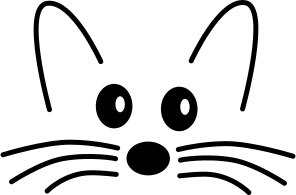
\includegraphics[width=1.4em]{squeak-logo}}}
\iftoshelse{
	\usepackage{marginnote}
		\renewcommand*{\marginfont}{\footnotesize}
	\newcommand{\vartriangleout}{\ifthenelse{\isodd{\thepage}}{\vartriangleright}{\vartriangleleft}}
	\newcommand{\dothisicon}{\fcolorbox{blue!65}{white}{\highlight{$\vartriangleout$}}}
	\newcommand{\dothis}[1]{%
		\noindent\par\noindent
		{\reversemarginpar
			\marginnote{\fcolorbox{blue!65}{white}{\highlight{$\vartriangleout$}}}}
		%\MarginLabel{do this}
		\noindent\emph{#1}
		\nopagebreak}
}{
	\newcommand{\dothisicon}{\raisebox{-.5ex}{
\includegraphics[height=1.2em]{pharo}}}
	\newcommand{\dothis}[1]{%
		\medskip
		\noindent\dothisicon
		\ifx#1\empty\else\quad\emph{#1}\fi
		\par\smallskip\nopagebreak}
}
%===> NEW VERSION <===
% NB: To use this in an individual chapter, you must set:
%\graphicspath{{figures/} {../figures/}}
% at the head of the chapter.  Don't forget the final /
%=============================================================
%:Reader hints (hint)
%
% Indicates a non-obvious consequence 
\newcommand{\hint}[1]{\vspace{1ex}\noindent\fbox{\textsc{Hint}} \emph{#1}}
%=================================================================
% graphics for Morphic handles
\newcommand{\grabHandle}{\raisebox{-0.2ex}{
\includegraphics[width=1em]{blackHandle}}}
\newcommand{\moveHandle}{\raisebox{-0.2ex}{
\includegraphics[width=1em]{moveHandle}}}
\newcommand{\debugHandle}{\raisebox{-0.2ex}{
\includegraphics[width=1em]{debugHandle}}}
%=============================================================
%:Highlighting Important stuff (doublebox)
%
% From Seaside book ...
\newsavebox{\SavedText}
\newlength{\InnerBoxRule}\setlength{\InnerBoxRule}{.75\fboxrule}
\newlength{\OuterBoxRule}\setlength{\OuterBoxRule}{1.5\fboxrule}
\newlength{\BoxSeparation}\setlength{\BoxSeparation}{1.5\fboxrule}
\addtolength{\BoxSeparation}{.5pt}
\newlength{\SaveBoxSep}\setlength{\SaveBoxSep}{2\fboxsep}
%
\newenvironment{doublebox}{\begin{lrbox}{\SavedText}
    \begin{minipage}{.75\textwidth}}
    {\end{minipage}\end{lrbox}\begin{center}
    \setlength{\fboxsep}{\BoxSeparation}\setlength{\fboxrule}{\OuterBoxRule}
    \fbox{\setlength{\fboxsep}{\SaveBoxSep}\setlength{\fboxrule}{\InnerBoxRule}%
      \fbox{\usebox{\SavedText}}}
  \end{center}}
% Use this:
\newcommand{\important}[1]{\begin{doublebox}#1\end{doublebox}}
%=============================================================
%:Section depth
\setcounter{secnumdepth}{2}
%% for this to happen start the file with
%\ifx\wholebook\relax\else
%% $Author$
% $Date$
% $Revision$

% HISTORY:
% 2006-10-31 - Oscar code macros
% ...

%=============================================================
% NB: documentclass must be set in main document.
% Allows book to be generated in multiple formats.
%=============================================================
%:Packages
\usepackage[T1]{fontenc}  %%%%%% really important to get the code directly in the text!
\usepackage{lmodern}
%\usepackage[scaled=0.85]{bookmanx} % needs another scale factor if used with \renewcommand{\sfdefault}{cmbr}
\usepackage{palatino}
\usepackage[scaled=0.85]{helvet}
\usepackage{microtype}
\usepackage{graphicx}
\usepackage{theorem}
\usepackage[english]{babel}
% ON: pdfsync breaks the use of p{width} for tabular columns!
\ifdefined\usepdfsync\usepackage{pdfsync}\fi % Requires texlive 2007
%=============================================================
%:More packages
%Stef should check which ones are used!
%\usepackage{picinpar}
%\usepackage{layout}
%\usepackage{color}
%\usepackage{enum}
%\usepackage{a4wide}
% \usepackage{fancyhdr}
\usepackage{ifthen}
\usepackage{float}
\usepackage{longtable}
\usepackage{makeidx}
\usepackage[nottoc]{tocbibind}
\usepackage{multicol}
\usepackage{booktabs}	% book-style tables
\usepackage{topcapt}	% enables \topcaption
\usepackage{multirow}
\usepackage{tabularx}
%\usepackage[bottom]{footmisc}
\usepackage{xspace}
\usepackage{alltt}
\usepackage{amssymb,textcomp}
\usepackage[usenames,dvipsnames]{color}
%\usepackage{colortbl}
\usepackage[hang]{subfigure}\makeatletter\def\p@subfigure{\thefigure\,}\makeatother
\usepackage{rotating}
\usepackage{enumitem}	% apb: allows more control over tags in enumerations
\usepackage{verbatim}     % for comment environment
\usepackage{varioref}	% for page references that work
\labelformat{footnote}{\thechapter--#1} % to distinguish citations from jurabib
\usepackage{needspace}
\usepackage{isodateo} % enable \isodate
\usepackage[newparttoc]{titlesec}
\usepackage{titletoc}
\usepackage{wrapfig}
\usepackage[
	super,
	citefull=first,
	authorformat={allreversed,and},
	titleformat={commasep,italic}
]{jurabib} % citations as footnotes
\usepackage[
	colorlinks=true,
	linkcolor=black,
	urlcolor=black,
	citecolor=black
]{hyperref}   % should come last
%=============================================================
%:PDF version
\pdfminorversion=3 % Set PDF to 1.3 for Lulu
%=============================================================
%:URL style
\makeatletter
\def\url@leostyle{%
  \@ifundefined{selectfont}{\def\UrlFont{\sf}}{\def\UrlFont{\sffamily}}}
\makeatother
% Now actually use the newly defined style.
\urlstyle{leo}
%=============================================================
%:Booleans
\newboolean{lulu}
\setboolean{lulu}{false}
\newcommand{\ifluluelse}[2]{\ifthenelse{\boolean{lulu}}{#1}{#2}}
%=============================================================
%:Names
\newcommand{\SUnit}{SUnit\xspace}
\newcommand{\sunit}{SUnit\xspace}
\newcommand{\xUnit}{$x$Unit\xspace}
\newcommand{\JUnit}{JUnit\xspace}
\newcommand{\st}{Smalltalk\xspace}
\newcommand{\pharo}{Pharo\xspace} % Use this, not \Pharo
%\newcommand{\sqmap}{SqueakMap\xspace}
\newcommand{\squeak}{Squeak\xspace} % use this, not \Squeak or \sq
\newcommand{\sqsrc}{SqueakSource\xspace}
\newcommand{\sbe}{\url{http://SqueakByExample.org}\xspace}
\newcommand{\pharoweb}{\url{http://pharo-project.org}\xspace}
\newcommand{\pbe}{\url{http://PharoByExample.org}\xspace}
\newcommand{\sba}{\url{http://SquareBracketAssociates.org}\xspace}
\newcommand{\bam}{\lct{Bounc\-ing\-Atoms\-Morph}\xspace}
%=============================================================
%:Markup macros for proof-reading
\usepackage[normalem]{ulem} % for \sout
\usepackage{xcolor}
\newcommand{\ra}{$\rightarrow$}
\newcommand{\ugh}[1]{\textcolor{red}{\uwave{#1}}} % please rephrase
\newcommand{\ins}[1]{\textcolor{blue}{\uline{#1}}} % please insert
\newcommand{\del}[1]{\textcolor{red}{\sout{#1}}} % please delete
\newcommand{\chg}[2]{\textcolor{red}{\sout{#1}}{\ra}\textcolor{blue}{\uline{#2}}} % please change
%=============================================================
%:Editorial comment macros
%\newcommand{\nnbb}[2]{
%    % \fbox{\bfseries\sffamily\scriptsize#1}
%    \fcolorbox{gray}{yellow}{\bfseries\sffamily\scriptsize#1}
%    {\sf\small$\blacktriangleright$\textit{#2}$\blacktriangleleft$}
%   }
\newcommand{\yellowbox}[1]{\fcolorbox{gray}{yellow}{\bfseries\sffamily\scriptsize#1}}
\newcommand{\triangles}[1]{{\sf\small$\blacktriangleright$\textit{#1}$\blacktriangleleft$}}
\newcommand{\nnbb}[2]{\yellowbox{#1} \triangles{#2}}
\newcommand{\fix}{\yellowbox{FIX!}}
\newcommand{\here}{\yellowbox{CONTINUE HERE!}}
% editor macros
\newcommand{\ab}[1]{\nnbb{Andrew}{#1}} % Black
\newcommand{\sd}[1]{\nnbb{St\'{e}f}{#1}} % Ducasse
\newcommand{\md}[1]{\nnbb{Marcus}{#1}} % Denker
\newcommand{\on}[1]{\nnbb{Oscar}{#1}} % Nierstrasz
\newcommand{\damien}[1]{\nnbb{Damien}{#1}} % Pollet
\newcommand{\lr}[1]{\nnbb{Lukas}{#1}} % Renggli
\newcommand{\orla}[1]{\nnbb{Orla}{#1}} % Greevy
\newcommand{\alex}[1]{\nnbb{Alex}{#1}} % Bergel
\newcommand{\alx}[1]{\nnbb{Alex}{#1}} % Bergel
\newcommand{\dr}[1]{\nnbb{David}{#1}} % Roethlisberger
\newcommand{\ja}[1]{\nnbb{Jannik}{#1}} % Laval
\newcommand{\jr}[1]{\nnbb{Jorge}{#1}} % Ressia
\newcommand{\fp}[1]{\nnbb{Fabrizio}{#1}} % Perin
\newcommand{\michael}[1]{\nnbb{Michael}{#1}} % Davies
\newcommand{\ew}[1]{\nnbb{Erwann}{#1}} % Wernli
\newcommand{\mb}[1]{\nnbb{Martial}{#1}} % Boniou
\newcommand{\hw}[1]{\nnbb{Hernan}{#1}} % Wilkinson
%=============================================================
%:Abbreviation macros
\newcommand{\ie}{\emph{i.e.},\xspace}
\newcommand{\eg}{\emph{e.g.},\xspace}
\newcommand{\etc}{etc.\xspace}
%=============================================================
%:Cross reference macros
\newcommand{\charef}[1]{Chapter~\ref{cha:#1}\xspace}
\newcommand{\secref}[1]{Section~\ref{sec:#1}\xspace}
\newcommand{\figref}[1]{Figure~\ref{fig:#1}\xspace}
\newcommand{\Figref}[1]{Figure~\ref{fig:#1}\xspace}
\newcommand{\appref}[1]{Appendix~\ref{app:#1}\xspace}
\newcommand{\tabref}[1]{Table~\ref{tab:#1}\xspace}
\newcommand{\faqref}[1]{FAQ~\ref{faq:#1}, p.~\pageref{faq:#1}\xspace}
% APB: I removed trailing \xspace commands from these macros because
% \xspace mostly doesn't work.  If you want a space after your
% references, type one!
% ON: xspace has always worked just fine for me!  Please leave them in.
%
\newcommand{\ruleref}[1]{\ref{rule:#1}\xspace}
%
\newcommand{\egref}[1]{example~\ref{eg:#1}\xspace}
\newcommand{\Egref}[1]{Example~\ref{eg:#1}\xspace}
%
\newcommand{\scrref}[1]{script~\ref{scr:#1}\xspace}
\newcommand{\Scrref}[1]{Script~\ref{scr:#1}\xspace}
\newcommand{\tscrref}[1]{the script~\ref{scr:#1}\xspace}
\newcommand{\Tscrref}[1]{The script~\ref{scr:#1}\xspace}
%
\newcommand{\mthref}[1]{method~\ref{mth:#1}\xspace}
\newcommand{\mthsref}[1]{methods~\ref{mth:#1}\xspace}
\newcommand{\Mthref}[1]{Method~\ref{mth:#1}\xspace}
\newcommand{\tmthref}[1]{the method~\ref{mth:#1}\xspace}
\newcommand{\Tmthref}[1]{The method~\ref{mth:#1}\xspace}
%
\newcommand{\clsref}[1]{class~\ref{cls:#1}\xspace}
\newcommand{\tclsref}[1]{the class~\ref{cls:#1}\xspace}
\newcommand{\Tclsref}[1]{The class~\ref{cls:#1}\xspace}

\newcommand{\chalabel}[1]{\label{cha:#1}}
\newcommand{\seclabel}[1]{\label{sec:#1}}
\newcommand{\figlabel}[1]{\label{fig:#1}}
\newcommand{\tablabel}[1]{\label{tab:#1}}
\newcommand{\rulelabel}[1]{\label{rule:#1}}
\newcommand{\eglabel}[1]{\label{eg:#1}}
\newcommand{\scrlabel}[1]{\label{scr:#1}}
\newcommand{\mthlabel}[1]{\label{mth:#1}}
\newcommand{\clslabel}[1]{\label{cls:#1}}
\newcommand{\faqlabel}[1]{\label{faq:#1}}
%=============================================================
%:Menu item macro
% for menu items, so we can change our minds on how to print them! (apb)
\definecolor{lightgray}{gray}{0.89}
\newcommand{\menu}[1]{{%
	\setlength{\fboxsep}{0pt}%
	\colorbox{lightgray}{{{\upshape\sffamily\strut \,#1\,}}}}}
\newcommand{\link}[1]{{%
	\fontfamily{lmr}\selectfont
 	\upshape{\sffamily \underline{#1}}}}
% For submenu items:
\newcommand{\go}{\,$\triangleright$\,}
% \newcommand{\go}{\,$\blacktriangleright$\,}
% For keyboard shortcuts:
%\newcommand{\short}[1]{\mbox{$\langle${\sc CMD}$\rangle$-#1}\xspace}
\newcommand{\short}[1]{\mbox{{\sc cmd}\hspace{0.08em}--\hspace{0.09em}#1}\xspace}
% For buttons:
\newcommand{\button}[1]{{%
	\setlength{\fboxsep}{0pt}%
	\fbox{{\upshape\sffamily\strut \,#1\,}}}}
% NB: The button macro does not work within captions -- incompatible with xcolor package :-(
\newcommand{\toolsflap}{\textit{Tools} flap\xspace}
%=============================================================
%:Mouse clicks
\newcommand{\click}{click\xspace} % RED
\newcommand{\actclick}{action-click\xspace} % YELLOW
\newcommand{\metaclick}{meta-click\xspace} % BLUE
\newcommand{\Click}{Click\xspace} % RED
\newcommand{\Actclick}{Action-click\xspace} % YELLOW
\newcommand{\Metaclick}{Meta-click\xspace} % BLUE
%=============================================================
%:ToSh macros
\newboolean{tosh}
\setboolean{tosh}{false}
\newcommand{\iftoshelse}[2]{\ifthenelse{\boolean{tosh}}{#1}{#2}}
%=============================================================
%:ToSh colors
%\newcommand{\highlightcolor}{\color{blue!65}}
%\newcommand{\boxcolor}{\color{gray!25}}
\newcommand{\highlight}[1]{\textcolor{blue!65}{#1}}
%\newcommand{\codecolor}{\color{blue!65}}
%%\setlength{\fboxrule}{2pt}
%\newcommand{\asPict}[1]{%
%	{\Large\highlight{#1}}}
%=============================================================
%:Reader cues (do this)
%
% Indicate something the reader should try out.
% \newcommand{\dothisicon}{\raisebox{-.5ex}{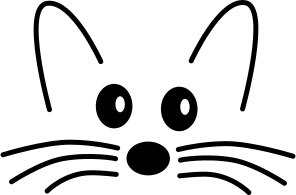
\includegraphics[width=1.4em]{squeak-logo}}}
\iftoshelse{
	\usepackage{marginnote}
		\renewcommand*{\marginfont}{\footnotesize}
	\newcommand{\vartriangleout}{\ifthenelse{\isodd{\thepage}}{\vartriangleright}{\vartriangleleft}}
	\newcommand{\dothisicon}{\fcolorbox{blue!65}{white}{\highlight{$\vartriangleout$}}}
	\newcommand{\dothis}[1]{%
		\noindent\par\noindent
		{\reversemarginpar
			\marginnote{\fcolorbox{blue!65}{white}{\highlight{$\vartriangleout$}}}}
		%\MarginLabel{do this}
		\noindent\emph{#1}
		\nopagebreak}
}{
	\newcommand{\dothisicon}{\raisebox{-.5ex}{
\includegraphics[height=1.2em]{pharo}}}
	\newcommand{\dothis}[1]{%
		\medskip
		\noindent\dothisicon
		\ifx#1\empty\else\quad\emph{#1}\fi
		\par\smallskip\nopagebreak}
}
%===> NEW VERSION <===
% NB: To use this in an individual chapter, you must set:
%\graphicspath{{figures/} {../figures/}}
% at the head of the chapter.  Don't forget the final /
%=============================================================
%:Reader hints (hint)
%
% Indicates a non-obvious consequence 
\newcommand{\hint}[1]{\vspace{1ex}\noindent\fbox{\textsc{Hint}} \emph{#1}}
%=================================================================
% graphics for Morphic handles
\newcommand{\grabHandle}{\raisebox{-0.2ex}{
\includegraphics[width=1em]{blackHandle}}}
\newcommand{\moveHandle}{\raisebox{-0.2ex}{
\includegraphics[width=1em]{moveHandle}}}
\newcommand{\debugHandle}{\raisebox{-0.2ex}{
\includegraphics[width=1em]{debugHandle}}}
%=============================================================
%:Highlighting Important stuff (doublebox)
%
% From Seaside book ...
\newsavebox{\SavedText}
\newlength{\InnerBoxRule}\setlength{\InnerBoxRule}{.75\fboxrule}
\newlength{\OuterBoxRule}\setlength{\OuterBoxRule}{1.5\fboxrule}
\newlength{\BoxSeparation}\setlength{\BoxSeparation}{1.5\fboxrule}
\addtolength{\BoxSeparation}{.5pt}
\newlength{\SaveBoxSep}\setlength{\SaveBoxSep}{2\fboxsep}
%
\newenvironment{doublebox}{\begin{lrbox}{\SavedText}
    \begin{minipage}{.75\textwidth}}
    {\end{minipage}\end{lrbox}\begin{center}
    \setlength{\fboxsep}{\BoxSeparation}\setlength{\fboxrule}{\OuterBoxRule}
    \fbox{\setlength{\fboxsep}{\SaveBoxSep}\setlength{\fboxrule}{\InnerBoxRule}%
      \fbox{\usebox{\SavedText}}}
  \end{center}}
% Use this:
\newcommand{\important}[1]{\begin{doublebox}#1\end{doublebox}}
%=============================================================
%:Section depth
\setcounter{secnumdepth}{2}
%% for this to happen start the file with
%\ifx\wholebook\relax\else
%% $Author$
% $Date$
% $Revision$

% HISTORY:
% 2006-10-31 - Oscar code macros
% ...

%=============================================================
% NB: documentclass must be set in main document.
% Allows book to be generated in multiple formats.
%=============================================================
%:Packages
\usepackage[T1]{fontenc}  %%%%%% really important to get the code directly in the text!
\usepackage{lmodern}
%\usepackage[scaled=0.85]{bookmanx} % needs another scale factor if used with \renewcommand{\sfdefault}{cmbr}
\usepackage{palatino}
\usepackage[scaled=0.85]{helvet}
\usepackage{microtype}
\usepackage{graphicx}
\usepackage{theorem}
\usepackage[english]{babel}
% ON: pdfsync breaks the use of p{width} for tabular columns!
\ifdefined\usepdfsync\usepackage{pdfsync}\fi % Requires texlive 2007
%=============================================================
%:More packages
%Stef should check which ones are used!
%\usepackage{picinpar}
%\usepackage{layout}
%\usepackage{color}
%\usepackage{enum}
%\usepackage{a4wide}
% \usepackage{fancyhdr}
\usepackage{ifthen}
\usepackage{float}
\usepackage{longtable}
\usepackage{makeidx}
\usepackage[nottoc]{tocbibind}
\usepackage{multicol}
\usepackage{booktabs}	% book-style tables
\usepackage{topcapt}	% enables \topcaption
\usepackage{multirow}
\usepackage{tabularx}
%\usepackage[bottom]{footmisc}
\usepackage{xspace}
\usepackage{alltt}
\usepackage{amssymb,textcomp}
\usepackage[usenames,dvipsnames]{color}
%\usepackage{colortbl}
\usepackage[hang]{subfigure}\makeatletter\def\p@subfigure{\thefigure\,}\makeatother
\usepackage{rotating}
\usepackage{enumitem}	% apb: allows more control over tags in enumerations
\usepackage{verbatim}     % for comment environment
\usepackage{varioref}	% for page references that work
\labelformat{footnote}{\thechapter--#1} % to distinguish citations from jurabib
\usepackage{needspace}
\usepackage{isodateo} % enable \isodate
\usepackage[newparttoc]{titlesec}
\usepackage{titletoc}
\usepackage{wrapfig}
\usepackage[
	super,
	citefull=first,
	authorformat={allreversed,and},
	titleformat={commasep,italic}
]{jurabib} % citations as footnotes
\usepackage[
	colorlinks=true,
	linkcolor=black,
	urlcolor=black,
	citecolor=black
]{hyperref}   % should come last
%=============================================================
%:PDF version
\pdfminorversion=3 % Set PDF to 1.3 for Lulu
%=============================================================
%:URL style
\makeatletter
\def\url@leostyle{%
  \@ifundefined{selectfont}{\def\UrlFont{\sf}}{\def\UrlFont{\sffamily}}}
\makeatother
% Now actually use the newly defined style.
\urlstyle{leo}
%=============================================================
%:Booleans
\newboolean{lulu}
\setboolean{lulu}{false}
\newcommand{\ifluluelse}[2]{\ifthenelse{\boolean{lulu}}{#1}{#2}}
%=============================================================
%:Names
\newcommand{\SUnit}{SUnit\xspace}
\newcommand{\sunit}{SUnit\xspace}
\newcommand{\xUnit}{$x$Unit\xspace}
\newcommand{\JUnit}{JUnit\xspace}
\newcommand{\st}{Smalltalk\xspace}
\newcommand{\pharo}{Pharo\xspace} % Use this, not \Pharo
%\newcommand{\sqmap}{SqueakMap\xspace}
\newcommand{\squeak}{Squeak\xspace} % use this, not \Squeak or \sq
\newcommand{\sqsrc}{SqueakSource\xspace}
\newcommand{\sbe}{\url{http://SqueakByExample.org}\xspace}
\newcommand{\pharoweb}{\url{http://pharo-project.org}\xspace}
\newcommand{\pbe}{\url{http://PharoByExample.org}\xspace}
\newcommand{\sba}{\url{http://SquareBracketAssociates.org}\xspace}
\newcommand{\bam}{\lct{Bounc\-ing\-Atoms\-Morph}\xspace}
%=============================================================
%:Markup macros for proof-reading
\usepackage[normalem]{ulem} % for \sout
\usepackage{xcolor}
\newcommand{\ra}{$\rightarrow$}
\newcommand{\ugh}[1]{\textcolor{red}{\uwave{#1}}} % please rephrase
\newcommand{\ins}[1]{\textcolor{blue}{\uline{#1}}} % please insert
\newcommand{\del}[1]{\textcolor{red}{\sout{#1}}} % please delete
\newcommand{\chg}[2]{\textcolor{red}{\sout{#1}}{\ra}\textcolor{blue}{\uline{#2}}} % please change
%=============================================================
%:Editorial comment macros
%\newcommand{\nnbb}[2]{
%    % \fbox{\bfseries\sffamily\scriptsize#1}
%    \fcolorbox{gray}{yellow}{\bfseries\sffamily\scriptsize#1}
%    {\sf\small$\blacktriangleright$\textit{#2}$\blacktriangleleft$}
%   }
\newcommand{\yellowbox}[1]{\fcolorbox{gray}{yellow}{\bfseries\sffamily\scriptsize#1}}
\newcommand{\triangles}[1]{{\sf\small$\blacktriangleright$\textit{#1}$\blacktriangleleft$}}
\newcommand{\nnbb}[2]{\yellowbox{#1} \triangles{#2}}
\newcommand{\fix}{\yellowbox{FIX!}}
\newcommand{\here}{\yellowbox{CONTINUE HERE!}}
% editor macros
\newcommand{\ab}[1]{\nnbb{Andrew}{#1}} % Black
\newcommand{\sd}[1]{\nnbb{St\'{e}f}{#1}} % Ducasse
\newcommand{\md}[1]{\nnbb{Marcus}{#1}} % Denker
\newcommand{\on}[1]{\nnbb{Oscar}{#1}} % Nierstrasz
\newcommand{\damien}[1]{\nnbb{Damien}{#1}} % Pollet
\newcommand{\lr}[1]{\nnbb{Lukas}{#1}} % Renggli
\newcommand{\orla}[1]{\nnbb{Orla}{#1}} % Greevy
\newcommand{\alex}[1]{\nnbb{Alex}{#1}} % Bergel
\newcommand{\alx}[1]{\nnbb{Alex}{#1}} % Bergel
\newcommand{\dr}[1]{\nnbb{David}{#1}} % Roethlisberger
\newcommand{\ja}[1]{\nnbb{Jannik}{#1}} % Laval
\newcommand{\jr}[1]{\nnbb{Jorge}{#1}} % Ressia
\newcommand{\fp}[1]{\nnbb{Fabrizio}{#1}} % Perin
\newcommand{\michael}[1]{\nnbb{Michael}{#1}} % Davies
\newcommand{\ew}[1]{\nnbb{Erwann}{#1}} % Wernli
\newcommand{\mb}[1]{\nnbb{Martial}{#1}} % Boniou
\newcommand{\hw}[1]{\nnbb{Hernan}{#1}} % Wilkinson
%=============================================================
%:Abbreviation macros
\newcommand{\ie}{\emph{i.e.},\xspace}
\newcommand{\eg}{\emph{e.g.},\xspace}
\newcommand{\etc}{etc.\xspace}
%=============================================================
%:Cross reference macros
\newcommand{\charef}[1]{Chapter~\ref{cha:#1}\xspace}
\newcommand{\secref}[1]{Section~\ref{sec:#1}\xspace}
\newcommand{\figref}[1]{Figure~\ref{fig:#1}\xspace}
\newcommand{\Figref}[1]{Figure~\ref{fig:#1}\xspace}
\newcommand{\appref}[1]{Appendix~\ref{app:#1}\xspace}
\newcommand{\tabref}[1]{Table~\ref{tab:#1}\xspace}
\newcommand{\faqref}[1]{FAQ~\ref{faq:#1}, p.~\pageref{faq:#1}\xspace}
% APB: I removed trailing \xspace commands from these macros because
% \xspace mostly doesn't work.  If you want a space after your
% references, type one!
% ON: xspace has always worked just fine for me!  Please leave them in.
%
\newcommand{\ruleref}[1]{\ref{rule:#1}\xspace}
%
\newcommand{\egref}[1]{example~\ref{eg:#1}\xspace}
\newcommand{\Egref}[1]{Example~\ref{eg:#1}\xspace}
%
\newcommand{\scrref}[1]{script~\ref{scr:#1}\xspace}
\newcommand{\Scrref}[1]{Script~\ref{scr:#1}\xspace}
\newcommand{\tscrref}[1]{the script~\ref{scr:#1}\xspace}
\newcommand{\Tscrref}[1]{The script~\ref{scr:#1}\xspace}
%
\newcommand{\mthref}[1]{method~\ref{mth:#1}\xspace}
\newcommand{\mthsref}[1]{methods~\ref{mth:#1}\xspace}
\newcommand{\Mthref}[1]{Method~\ref{mth:#1}\xspace}
\newcommand{\tmthref}[1]{the method~\ref{mth:#1}\xspace}
\newcommand{\Tmthref}[1]{The method~\ref{mth:#1}\xspace}
%
\newcommand{\clsref}[1]{class~\ref{cls:#1}\xspace}
\newcommand{\tclsref}[1]{the class~\ref{cls:#1}\xspace}
\newcommand{\Tclsref}[1]{The class~\ref{cls:#1}\xspace}

\newcommand{\chalabel}[1]{\label{cha:#1}}
\newcommand{\seclabel}[1]{\label{sec:#1}}
\newcommand{\figlabel}[1]{\label{fig:#1}}
\newcommand{\tablabel}[1]{\label{tab:#1}}
\newcommand{\rulelabel}[1]{\label{rule:#1}}
\newcommand{\eglabel}[1]{\label{eg:#1}}
\newcommand{\scrlabel}[1]{\label{scr:#1}}
\newcommand{\mthlabel}[1]{\label{mth:#1}}
\newcommand{\clslabel}[1]{\label{cls:#1}}
\newcommand{\faqlabel}[1]{\label{faq:#1}}
%=============================================================
%:Menu item macro
% for menu items, so we can change our minds on how to print them! (apb)
\definecolor{lightgray}{gray}{0.89}
\newcommand{\menu}[1]{{%
	\setlength{\fboxsep}{0pt}%
	\colorbox{lightgray}{{{\upshape\sffamily\strut \,#1\,}}}}}
\newcommand{\link}[1]{{%
	\fontfamily{lmr}\selectfont
 	\upshape{\sffamily \underline{#1}}}}
% For submenu items:
\newcommand{\go}{\,$\triangleright$\,}
% \newcommand{\go}{\,$\blacktriangleright$\,}
% For keyboard shortcuts:
%\newcommand{\short}[1]{\mbox{$\langle${\sc CMD}$\rangle$-#1}\xspace}
\newcommand{\short}[1]{\mbox{{\sc cmd}\hspace{0.08em}--\hspace{0.09em}#1}\xspace}
% For buttons:
\newcommand{\button}[1]{{%
	\setlength{\fboxsep}{0pt}%
	\fbox{{\upshape\sffamily\strut \,#1\,}}}}
% NB: The button macro does not work within captions -- incompatible with xcolor package :-(
\newcommand{\toolsflap}{\textit{Tools} flap\xspace}
%=============================================================
%:Mouse clicks
\newcommand{\click}{click\xspace} % RED
\newcommand{\actclick}{action-click\xspace} % YELLOW
\newcommand{\metaclick}{meta-click\xspace} % BLUE
\newcommand{\Click}{Click\xspace} % RED
\newcommand{\Actclick}{Action-click\xspace} % YELLOW
\newcommand{\Metaclick}{Meta-click\xspace} % BLUE
%=============================================================
%:ToSh macros
\newboolean{tosh}
\setboolean{tosh}{false}
\newcommand{\iftoshelse}[2]{\ifthenelse{\boolean{tosh}}{#1}{#2}}
%=============================================================
%:ToSh colors
%\newcommand{\highlightcolor}{\color{blue!65}}
%\newcommand{\boxcolor}{\color{gray!25}}
\newcommand{\highlight}[1]{\textcolor{blue!65}{#1}}
%\newcommand{\codecolor}{\color{blue!65}}
%%\setlength{\fboxrule}{2pt}
%\newcommand{\asPict}[1]{%
%	{\Large\highlight{#1}}}
%=============================================================
%:Reader cues (do this)
%
% Indicate something the reader should try out.
% \newcommand{\dothisicon}{\raisebox{-.5ex}{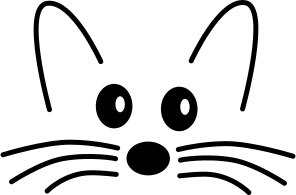
\includegraphics[width=1.4em]{squeak-logo}}}
\iftoshelse{
	\usepackage{marginnote}
		\renewcommand*{\marginfont}{\footnotesize}
	\newcommand{\vartriangleout}{\ifthenelse{\isodd{\thepage}}{\vartriangleright}{\vartriangleleft}}
	\newcommand{\dothisicon}{\fcolorbox{blue!65}{white}{\highlight{$\vartriangleout$}}}
	\newcommand{\dothis}[1]{%
		\noindent\par\noindent
		{\reversemarginpar
			\marginnote{\fcolorbox{blue!65}{white}{\highlight{$\vartriangleout$}}}}
		%\MarginLabel{do this}
		\noindent\emph{#1}
		\nopagebreak}
}{
	\newcommand{\dothisicon}{\raisebox{-.5ex}{
\includegraphics[height=1.2em]{pharo}}}
	\newcommand{\dothis}[1]{%
		\medskip
		\noindent\dothisicon
		\ifx#1\empty\else\quad\emph{#1}\fi
		\par\smallskip\nopagebreak}
}
%===> NEW VERSION <===
% NB: To use this in an individual chapter, you must set:
%\graphicspath{{figures/} {../figures/}}
% at the head of the chapter.  Don't forget the final /
%=============================================================
%:Reader hints (hint)
%
% Indicates a non-obvious consequence 
\newcommand{\hint}[1]{\vspace{1ex}\noindent\fbox{\textsc{Hint}} \emph{#1}}
%=================================================================
% graphics for Morphic handles
\newcommand{\grabHandle}{\raisebox{-0.2ex}{
\includegraphics[width=1em]{blackHandle}}}
\newcommand{\moveHandle}{\raisebox{-0.2ex}{
\includegraphics[width=1em]{moveHandle}}}
\newcommand{\debugHandle}{\raisebox{-0.2ex}{
\includegraphics[width=1em]{debugHandle}}}
%=============================================================
%:Highlighting Important stuff (doublebox)
%
% From Seaside book ...
\newsavebox{\SavedText}
\newlength{\InnerBoxRule}\setlength{\InnerBoxRule}{.75\fboxrule}
\newlength{\OuterBoxRule}\setlength{\OuterBoxRule}{1.5\fboxrule}
\newlength{\BoxSeparation}\setlength{\BoxSeparation}{1.5\fboxrule}
\addtolength{\BoxSeparation}{.5pt}
\newlength{\SaveBoxSep}\setlength{\SaveBoxSep}{2\fboxsep}
%
\newenvironment{doublebox}{\begin{lrbox}{\SavedText}
    \begin{minipage}{.75\textwidth}}
    {\end{minipage}\end{lrbox}\begin{center}
    \setlength{\fboxsep}{\BoxSeparation}\setlength{\fboxrule}{\OuterBoxRule}
    \fbox{\setlength{\fboxsep}{\SaveBoxSep}\setlength{\fboxrule}{\InnerBoxRule}%
      \fbox{\usebox{\SavedText}}}
  \end{center}}
% Use this:
\newcommand{\important}[1]{\begin{doublebox}#1\end{doublebox}}
%=============================================================
%:Section depth
\setcounter{secnumdepth}{2}
%% for this to happen start the file with
%\ifx\wholebook\relax\else
%\input{../common.tex}
%\begin{document}
%\fi
% and terminate by
% \ifx\wholebook\relax\else\end{document}\fi

\DeclareGraphicsExtensions{.pdf, .jpg, .png}
%=============================================================
%:PDF setup
\hypersetup{
%   a4paper,
%   pdfstartview=FitV,
%   colorlinks,
%   linkcolor=darkblue,
%   citecolor=darkblue,
   pdftitle={Pharo by Example},
   pdfauthor={Andrew P. Black, St\'ephane Ducasse,	Oscar Nierstrasz,
Damien Pollet},
   pdfkeywords={Smalltalk, Squeak, Object-Oriented Programming, OOP},
   pdfsubject={Computer Science}
}
%=============================================================
%:Page layout and appearance
%
% \renewcommand{\headrulewidth}{0pt}
\renewcommand{\chaptermark}[1]{\markboth{#1}{}}
\renewcommand{\sectionmark}[1]{\markright{\thesection\ #1}}
\renewpagestyle{plain}[\small\itshape]{%
	\setheadrule{0pt}%
	\sethead[][][]{}{}{}%
	\setfoot[][][]{}{}{}}
\renewpagestyle{headings}[\small\itshape]{%
	\setheadrule{0pt}%
	\setmarks{chapter}{section}%
	\sethead[\thepage][][\chaptertitle]{\sectiontitle}{}{\thepage}%
	\setfoot[][][]{}{}{}}
%=============================================================
%:Title section setup and TOC numbering depth
\setcounter{secnumdepth}{1}
\setcounter{tocdepth}{1}
\titleformat{\part}[display]{\centering}{\huge\partname\ \thepart}{1em}{\Huge\textbf}[]
\titleformat{\chapter}[display]{}{\huge\chaptertitlename\ \thechapter}{1em}{\Huge\raggedright\textbf}[]
\titlecontents{part}[3pc]{%
		\pagebreak[2]\addvspace{1em plus.4em minus.2em}%
		\leavevmode\large\bfseries}
	{\contentslabel{3pc}}{\hspace*{-3pc}}
	{}[\nopagebreak]
\titlecontents{chapter}[3pc]{%
		\pagebreak[0]\addvspace{1em plus.2em minus.2em}%
		\leavevmode\bfseries}
	{\contentslabel{3pc}}{}
	{\hfill\contentspage}[\nopagebreak]
\dottedcontents{section}[3pc]{}{3pc}{1pc}
\dottedcontents{subsection}[3pc]{}{0pc}{1pc}
% \dottedcontents{subsection}[4.5em]{}{0pt}{1pc}
% Make \cleardoublepage insert really blank pages http://www.tex.ac.uk/cgi-bin/texfaq2html?label=reallyblank
\let\origdoublepage\cleardoublepage
\newcommand{\clearemptydoublepage}{%
  \clearpage
  {\pagestyle{empty}\origdoublepage}}
\let\cleardoublepage\clearemptydoublepage % see http://www.tex.ac.uk/cgi-bin/texfaq2html?label=patch
%=============================================================
%:FAQ macros (for FAQ chapter)
\newtheorem{faq}{FAQ}
\newcommand{\answer}{\paragraph{Answer}\ }
%=============================================================
%:Listings package configuration
% \newcommand{\caret}{\makebox{\raisebox{0.4ex}{\footnotesize{$\wedge$}}}}
\newcommand{\caret}{\^\,}
\newcommand{\escape}{{\sf \textbackslash}}
\definecolor{source}{gray}{0.95}
\usepackage{listings}
\lstdefinelanguage{Smalltalk}{
%  morekeywords={self,super,true,false,nil,thisContext}, % This is overkill
  morestring=[d]',
  morecomment=[s]{"}{"},
  alsoletter={\#:},
  escapechar={!},
  literate=
    {BANG}{!}1
    {CARET}{\^}1
    {UNDERSCORE}{\_}1
    {\\st}{Smalltalk}9 % convenience -- in case \st occurs in code
    % {'}{{\textquotesingle}}1 % replaced by upquote=true in \lstset
    {_}{{$\leftarrow$}}1
    {>>>}{{\sep}}1
    {^}{{$\uparrow$}}1
    {~}{{$\sim$}}1
    {-}{{\textminus}}1 %{-}{\hspace{-0.13em}}{-}}1  % the goal is to make - the same width as +
    % {+}{\sf+}1 %{\raisebox{0.08ex}{+}}}1      % and to raise + off the baseline to match -
    {-->}{{\quad$\longrightarrow$\quad}}3
	, % Don't forget the comma at the end!
  tabsize=4
}[keywords,comments,strings]

\lstset{language=Smalltalk,
	basicstyle=\sffamily,
	keywordstyle=\color{black}\bfseries,
	% stringstyle=\ttfamily, % Ugly! do we really want this? -- on
	mathescape=true,
	showstringspaces=false,
	keepspaces=true,
	breaklines=true,
	breakautoindent=true,
	backgroundcolor=\color{source},
	lineskip={-1pt}, % Ugly hack
	upquote=true, % straight quote; requires textcomp package
	columns=fullflexible} % no fixed width fonts
% In-line code (literal)
% Normally use this for all in-line code:
\newcommand{\ct}{\lstinline[mathescape=false,backgroundcolor=\color{white},basicstyle={\sffamily\upshape}]}
% apb 2007.8.28 added the \upshape declaration to avoid getting italicized code in \dothis{ } sections.
% In-line code (latex enabled)
% Use this only in special situations where \ct does not work
% (within section headings ...):
\newcommand{\lct}[1]{{\textsf{\textup{#1}}}}
% Use these for system categories and protocols:
\newcommand{\scat}[1]{\emph{\textsf{#1}}\xspace}
\newcommand{\pkg}[1]{\emph{\textsf{#1}}\xspace}
\newcommand{\prot}[1]{\emph{\textsf{#1}}\xspace}
% Code environments
% NB: the arg is for tests
% Only code and example environments may be tests
\lstnewenvironment{code}[1]{%
	\lstset{%
		% frame=lines,
		frame=single,
		framerule=0pt,
		mathescape=false
	}
}{}
\def\ignoredollar#1{}
%=============================================================
%:Code environments (method, script ...)
% NB: the third arg is for tests
% Only code and example environments may be tests
\lstnewenvironment{example}[3][defaultlabel]{%
	\renewcommand{\lstlistingname}{Example}%
	\lstset{
		% frame=lines,
		frame=single,
		framerule=0pt,
		mathescape=false,
		caption={\emph{#2}},
		label={eg:#1}
	}
}{}
\lstnewenvironment{script}[2][defaultlabel]{%
\renewcommand{\lstlistingname}{Script}%
	\lstset{
		% frame=lines,
		frame=single,
		framerule=0pt,
		mathescape=false,
		name={Script},
		caption={\emph{#2}},
		label={scr:#1}
	}
}{}
\lstnewenvironment{method}[2][defaultlabel]{%
	\renewcommand{\lstlistingname}{Method}%
	\lstset{
		% frame=lines,
		frame=single,
		framerule=0pt,
		mathescape=false,
		name={Method},
		caption={\emph{#2}},
		label={mth:#1}
	}
}{}
\lstnewenvironment{methods}[2][defaultlabel]{% just for multiple methods at once
	\renewcommand{\lstlistingname}{Methods}%
	\lstset{
		% frame=lines,
		frame=single,
		framerule=0pt,
		mathescape=false,
		name={Method},
		caption={\emph{#2}},
		label={mth:#1}
	}
}{}
\lstnewenvironment{numMethod}[2][defaultlabel]{%
	\renewcommand{\lstlistingname}{Method}%
	\lstset{
		numbers=left,
		numberstyle={\tiny\sffamily},
		% frame=lines,
		frame=single,
		framerule=0pt,
		mathescape=false,
		name={Method},
		caption={\emph{#2}},
		label={mth:#1}
	}
}{}
\lstnewenvironment{classdef}[2][defaultlabel]{%
	\renewcommand{\lstlistingname}{Class}%
	\lstset{
		% frame=lines,
		frame=single,
		framerule=0pt,
		mathescape=false,
		name={Class},
		caption={\emph{#2}},
		label={cls:#1}
	}
}{}
%=============================================================
%:Reserving space
% Usually need one more line than the actual lines of code
\newcommand{\needlines}[1]{\Needspace{#1\baselineskip}}
%=============================================================
%:Indexing macros
% Macros ending with "ind" generate text as well as an index entry
% Macros ending with "index" *only* generate an index entry
\newcommand{\ind}[1]{\index{#1}#1\xspace} % plain text
\newcommand{\subind}[2]{\index{#1!#2}#2\xspace} % show #2, subindex under #1
\newcommand{\emphind}[1]{\index{#1}\emph{#1}\xspace} % emph #1
\newcommand{\emphsubind}[2]{\index{#1!#2}\emph{#2}\xspace} % show emph #2, subindex inder #1
\newcommand{\scatind}[1]{\index{#1@\textsf{#1} (category)}\scat{#1}} % category
\newcommand{\pkgind}[1]{\index{#1@\textsf{#1} (package)}\pkg{#1}} % package
\newcommand{\protind}[1]{\index{#1@\textsf{#1} (protocol)}\prot{#1}} % protocol
\newcommand{\clsind}[1]{\index{#1@\textsf{#1} (class)}\ct{#1}\xspace}
% \newcommand{\clsind}[1]{\index{#1!\#@(class)}\ct{#1}\xspace} % class
\newcommand{\clsindplural}[1]{\index{#1!\#@(class)}\ct{#1}s\xspace} % class
\newcommand{\cvind}[1]{\index{#1@\textsf{#1} (class variable)}\ct{#1}\xspace} % class var
\newcommand{\glbind}[1]{\index{#1@\textsf{#1} (global)}\ct{#1}\xspace} % global
\newcommand{\patind}[1]{\index{#1@#1 (pattern)}\ct{#1}\xspace} % pattern
\newcommand{\pvind}[1]{\index{#1@\textsf{#1} (pseudo variable)}\ct{#1}\xspace} % pseudo var
\newcommand{\clsmthind}[2]{\index{#1!#2@\ct{#2}}\ct{#1>>>#2}\xspace} % class + method name
\newcommand{\mthind}[2]{\index{#1!#2@\ct{#2}}\ct{#2}\xspace} % show method name only
\newcommand{\lmthind}[2]{\index{#1!#2@\ct{#2}}\lct{#2}\xspace} % show method name only
\newcommand{\cmind}[2]{\index{#1!#2@\ct{#2}}\ct{#1>>>#2}\xspace} % show class>>method
\newcommand{\lcmind}[2]{\index{#1!#2@\ct{#2}}\lct{#1>>>#2}\xspace} % show class>>method
\newcommand{\toolsflapind}{\index{Tools flap}\toolsflap} % index tools flap
% The following only generate an index entry:
% \newcommand{\clsindex}[1]{\index{#1@\textsf{#1} (class)}}
\newcommand{\clsindex}[1]{\index{#1!\#@(class)}} % class
\newcommand{\mthindex}[2]{\index{#1!#2@\ct{#2}}} % method
\newcommand{\cmindex}[2]{\index{#1!#2@\ct{#2}}} % class>>method
\newcommand{\cvindex}[1]{\index{#1@\textsf{#1} (class variable)}} % class var
\newcommand{\glbindex}[1]{\index{#1@\textsf{#1} (global)}}% global
\newcommand{\pvindex}[1]{\index{#1@\textsf{#1} (pseudo variable)}}% pseudo var
\newcommand{\seeindex}[2]{\index{#1|see{#2}}} % #1, see #2
\newcommand{\scatindex}[1]{\index{#1@\textsf{#1} (category)}} % category
\newcommand{\pkgindex}[1]{\index{#1@\textsf{#1} (package)}} % package
\newcommand{\protindex}[1]{\index{#1@\textsf{#1} (protocol)}} % protocol
% How can we have the main entry page numbers in bold yet not break the hyperlink?
\newcommand{\boldidx}[1]{{\bf #1}} % breaks hyperlink
%\newcommand{\indmain}[1]{\index{#1|boldidx}#1\xspace} % plain text, main entry
%\newcommand{\emphsubindmain}[2]{\index{#1!#2|boldidx}\emph{#2}\xspace} % subindex, main entry
%\newcommand{\subindmain}[2]{\index{#1!#2|boldidx}#2\xspace} % subindex, main entry
%\newcommand{\clsindmain}[1]{\index{#1@\textsf{#1} (class)|boldidx}\ct{#1}\xspace}
%\newcommand{\clsindmain}[1]{\index{#1!\#@(class)|boldidx}\ct{#1}\xspace} % class main
%\newcommand{\indexmain}[1]{\index{#1|boldidx}} % main index entry only
\newcommand{\indmain}[1]{\index{#1}#1\xspace} % The main index entry for this item
\newcommand{\emphsubindmain}[2]{\index{#1!#2}\emph{#2}\xspace} % subindex, main entry
\newcommand{\subindmain}[2]{\index{#1!#2}#2\xspace} % subindex, main entry
%\newcommand{\clsindmain}[1]{\index{#1@\textsf{#1} (class)}\ct{#1}\xspace}
\newcommand{\clsindmain}[1]{\index{#1!\#@(class)}\ct{#1}\xspace} % class main
\newcommand{\clsindexmain}[1]{\index{#1!\#@(class)}} % class main index only
\newcommand{\indexmain}[1]{\index{#1}} 
%=============================================================
%:Code macros
% some constants
\newcommand{\codesize}{\small}
\newcommand{\codefont}{\sffamily}
%\newcommand{\cat}[1]{\textit{In category #1}}%%To remove later
\newlength{\scriptindent}
\setlength{\scriptindent}{.3cm}
%% Method presentation constants
\newlength{\methodindent}
\newlength{\methodwordlength}
\newlength{\aftermethod}
\setlength{\methodindent}{0.2cm}
\settowidth{\methodwordlength}{\ M\'ethode\ }
%=============================================================
%:Smalltalk macros
%\newcommand{\sep}{{$\gg$}}
\newcommand{\sep}{\mbox{>>}}
\newcommand{\self}{\lct{self}\xspace}
\newcommand{\super}{\lct{super}\xspace}
\newcommand{\nil}{\lct{nil}\xspace}
%=============================================================
% be less conservative about float placement
% these commands are from http://www.tex.ac.uk/cgi-bin/texfaq2html?label=floats
\renewcommand{\topfraction}{.9}
\renewcommand{\bottomfraction}{.9}
\renewcommand{\textfraction}{.1}
\renewcommand{\floatpagefraction}{.85}
\renewcommand{\dbltopfraction}{.66}
\renewcommand{\dblfloatpagefraction}{.85}
\setcounter{topnumber}{9}
\setcounter{bottomnumber}{9}
\setcounter{totalnumber}{20}
\setcounter{dbltopnumber}{9}
%=============================================================
% apb doesn't like paragraphs to run in to each other without a break
\parskip 1ex
%=============================================================
%:Stuff to check, merge or deprecate
%\setlength{\marginparsep}{2mm}
%\renewcommand{\baselinestretch}{1.1}
%=============================================================

%\begin{document}
%\fi
% and terminate by
% \ifx\wholebook\relax\else\end{document}\fi

\DeclareGraphicsExtensions{.pdf, .jpg, .png}
%=============================================================
%:PDF setup
\hypersetup{
%   a4paper,
%   pdfstartview=FitV,
%   colorlinks,
%   linkcolor=darkblue,
%   citecolor=darkblue,
   pdftitle={Pharo by Example},
   pdfauthor={Andrew P. Black, St\'ephane Ducasse,	Oscar Nierstrasz,
Damien Pollet},
   pdfkeywords={Smalltalk, Squeak, Object-Oriented Programming, OOP},
   pdfsubject={Computer Science}
}
%=============================================================
%:Page layout and appearance
%
% \renewcommand{\headrulewidth}{0pt}
\renewcommand{\chaptermark}[1]{\markboth{#1}{}}
\renewcommand{\sectionmark}[1]{\markright{\thesection\ #1}}
\renewpagestyle{plain}[\small\itshape]{%
	\setheadrule{0pt}%
	\sethead[][][]{}{}{}%
	\setfoot[][][]{}{}{}}
\renewpagestyle{headings}[\small\itshape]{%
	\setheadrule{0pt}%
	\setmarks{chapter}{section}%
	\sethead[\thepage][][\chaptertitle]{\sectiontitle}{}{\thepage}%
	\setfoot[][][]{}{}{}}
%=============================================================
%:Title section setup and TOC numbering depth
\setcounter{secnumdepth}{1}
\setcounter{tocdepth}{1}
\titleformat{\part}[display]{\centering}{\huge\partname\ \thepart}{1em}{\Huge\textbf}[]
\titleformat{\chapter}[display]{}{\huge\chaptertitlename\ \thechapter}{1em}{\Huge\raggedright\textbf}[]
\titlecontents{part}[3pc]{%
		\pagebreak[2]\addvspace{1em plus.4em minus.2em}%
		\leavevmode\large\bfseries}
	{\contentslabel{3pc}}{\hspace*{-3pc}}
	{}[\nopagebreak]
\titlecontents{chapter}[3pc]{%
		\pagebreak[0]\addvspace{1em plus.2em minus.2em}%
		\leavevmode\bfseries}
	{\contentslabel{3pc}}{}
	{\hfill\contentspage}[\nopagebreak]
\dottedcontents{section}[3pc]{}{3pc}{1pc}
\dottedcontents{subsection}[3pc]{}{0pc}{1pc}
% \dottedcontents{subsection}[4.5em]{}{0pt}{1pc}
% Make \cleardoublepage insert really blank pages http://www.tex.ac.uk/cgi-bin/texfaq2html?label=reallyblank
\let\origdoublepage\cleardoublepage
\newcommand{\clearemptydoublepage}{%
  \clearpage
  {\pagestyle{empty}\origdoublepage}}
\let\cleardoublepage\clearemptydoublepage % see http://www.tex.ac.uk/cgi-bin/texfaq2html?label=patch
%=============================================================
%:FAQ macros (for FAQ chapter)
\newtheorem{faq}{FAQ}
\newcommand{\answer}{\paragraph{Answer}\ }
%=============================================================
%:Listings package configuration
% \newcommand{\caret}{\makebox{\raisebox{0.4ex}{\footnotesize{$\wedge$}}}}
\newcommand{\caret}{\^\,}
\newcommand{\escape}{{\sf \textbackslash}}
\definecolor{source}{gray}{0.95}
\usepackage{listings}
\lstdefinelanguage{Smalltalk}{
%  morekeywords={self,super,true,false,nil,thisContext}, % This is overkill
  morestring=[d]',
  morecomment=[s]{"}{"},
  alsoletter={\#:},
  escapechar={!},
  literate=
    {BANG}{!}1
    {CARET}{\^}1
    {UNDERSCORE}{\_}1
    {\\st}{Smalltalk}9 % convenience -- in case \st occurs in code
    % {'}{{\textquotesingle}}1 % replaced by upquote=true in \lstset
    {_}{{$\leftarrow$}}1
    {>>>}{{\sep}}1
    {^}{{$\uparrow$}}1
    {~}{{$\sim$}}1
    {-}{{\textminus}}1 %{-}{\hspace{-0.13em}}{-}}1  % the goal is to make - the same width as +
    % {+}{\sf+}1 %{\raisebox{0.08ex}{+}}}1      % and to raise + off the baseline to match -
    {-->}{{\quad$\longrightarrow$\quad}}3
	, % Don't forget the comma at the end!
  tabsize=4
}[keywords,comments,strings]

\lstset{language=Smalltalk,
	basicstyle=\sffamily,
	keywordstyle=\color{black}\bfseries,
	% stringstyle=\ttfamily, % Ugly! do we really want this? -- on
	mathescape=true,
	showstringspaces=false,
	keepspaces=true,
	breaklines=true,
	breakautoindent=true,
	backgroundcolor=\color{source},
	lineskip={-1pt}, % Ugly hack
	upquote=true, % straight quote; requires textcomp package
	columns=fullflexible} % no fixed width fonts
% In-line code (literal)
% Normally use this for all in-line code:
\newcommand{\ct}{\lstinline[mathescape=false,backgroundcolor=\color{white},basicstyle={\sffamily\upshape}]}
% apb 2007.8.28 added the \upshape declaration to avoid getting italicized code in \dothis{ } sections.
% In-line code (latex enabled)
% Use this only in special situations where \ct does not work
% (within section headings ...):
\newcommand{\lct}[1]{{\textsf{\textup{#1}}}}
% Use these for system categories and protocols:
\newcommand{\scat}[1]{\emph{\textsf{#1}}\xspace}
\newcommand{\pkg}[1]{\emph{\textsf{#1}}\xspace}
\newcommand{\prot}[1]{\emph{\textsf{#1}}\xspace}
% Code environments
% NB: the arg is for tests
% Only code and example environments may be tests
\lstnewenvironment{code}[1]{%
	\lstset{%
		% frame=lines,
		frame=single,
		framerule=0pt,
		mathescape=false
	}
}{}
\def\ignoredollar#1{}
%=============================================================
%:Code environments (method, script ...)
% NB: the third arg is for tests
% Only code and example environments may be tests
\lstnewenvironment{example}[3][defaultlabel]{%
	\renewcommand{\lstlistingname}{Example}%
	\lstset{
		% frame=lines,
		frame=single,
		framerule=0pt,
		mathescape=false,
		caption={\emph{#2}},
		label={eg:#1}
	}
}{}
\lstnewenvironment{script}[2][defaultlabel]{%
\renewcommand{\lstlistingname}{Script}%
	\lstset{
		% frame=lines,
		frame=single,
		framerule=0pt,
		mathescape=false,
		name={Script},
		caption={\emph{#2}},
		label={scr:#1}
	}
}{}
\lstnewenvironment{method}[2][defaultlabel]{%
	\renewcommand{\lstlistingname}{Method}%
	\lstset{
		% frame=lines,
		frame=single,
		framerule=0pt,
		mathescape=false,
		name={Method},
		caption={\emph{#2}},
		label={mth:#1}
	}
}{}
\lstnewenvironment{methods}[2][defaultlabel]{% just for multiple methods at once
	\renewcommand{\lstlistingname}{Methods}%
	\lstset{
		% frame=lines,
		frame=single,
		framerule=0pt,
		mathescape=false,
		name={Method},
		caption={\emph{#2}},
		label={mth:#1}
	}
}{}
\lstnewenvironment{numMethod}[2][defaultlabel]{%
	\renewcommand{\lstlistingname}{Method}%
	\lstset{
		numbers=left,
		numberstyle={\tiny\sffamily},
		% frame=lines,
		frame=single,
		framerule=0pt,
		mathescape=false,
		name={Method},
		caption={\emph{#2}},
		label={mth:#1}
	}
}{}
\lstnewenvironment{classdef}[2][defaultlabel]{%
	\renewcommand{\lstlistingname}{Class}%
	\lstset{
		% frame=lines,
		frame=single,
		framerule=0pt,
		mathescape=false,
		name={Class},
		caption={\emph{#2}},
		label={cls:#1}
	}
}{}
%=============================================================
%:Reserving space
% Usually need one more line than the actual lines of code
\newcommand{\needlines}[1]{\Needspace{#1\baselineskip}}
%=============================================================
%:Indexing macros
% Macros ending with "ind" generate text as well as an index entry
% Macros ending with "index" *only* generate an index entry
\newcommand{\ind}[1]{\index{#1}#1\xspace} % plain text
\newcommand{\subind}[2]{\index{#1!#2}#2\xspace} % show #2, subindex under #1
\newcommand{\emphind}[1]{\index{#1}\emph{#1}\xspace} % emph #1
\newcommand{\emphsubind}[2]{\index{#1!#2}\emph{#2}\xspace} % show emph #2, subindex inder #1
\newcommand{\scatind}[1]{\index{#1@\textsf{#1} (category)}\scat{#1}} % category
\newcommand{\pkgind}[1]{\index{#1@\textsf{#1} (package)}\pkg{#1}} % package
\newcommand{\protind}[1]{\index{#1@\textsf{#1} (protocol)}\prot{#1}} % protocol
\newcommand{\clsind}[1]{\index{#1@\textsf{#1} (class)}\ct{#1}\xspace}
% \newcommand{\clsind}[1]{\index{#1!\#@(class)}\ct{#1}\xspace} % class
\newcommand{\clsindplural}[1]{\index{#1!\#@(class)}\ct{#1}s\xspace} % class
\newcommand{\cvind}[1]{\index{#1@\textsf{#1} (class variable)}\ct{#1}\xspace} % class var
\newcommand{\glbind}[1]{\index{#1@\textsf{#1} (global)}\ct{#1}\xspace} % global
\newcommand{\patind}[1]{\index{#1@#1 (pattern)}\ct{#1}\xspace} % pattern
\newcommand{\pvind}[1]{\index{#1@\textsf{#1} (pseudo variable)}\ct{#1}\xspace} % pseudo var
\newcommand{\clsmthind}[2]{\index{#1!#2@\ct{#2}}\ct{#1>>>#2}\xspace} % class + method name
\newcommand{\mthind}[2]{\index{#1!#2@\ct{#2}}\ct{#2}\xspace} % show method name only
\newcommand{\lmthind}[2]{\index{#1!#2@\ct{#2}}\lct{#2}\xspace} % show method name only
\newcommand{\cmind}[2]{\index{#1!#2@\ct{#2}}\ct{#1>>>#2}\xspace} % show class>>method
\newcommand{\lcmind}[2]{\index{#1!#2@\ct{#2}}\lct{#1>>>#2}\xspace} % show class>>method
\newcommand{\toolsflapind}{\index{Tools flap}\toolsflap} % index tools flap
% The following only generate an index entry:
% \newcommand{\clsindex}[1]{\index{#1@\textsf{#1} (class)}}
\newcommand{\clsindex}[1]{\index{#1!\#@(class)}} % class
\newcommand{\mthindex}[2]{\index{#1!#2@\ct{#2}}} % method
\newcommand{\cmindex}[2]{\index{#1!#2@\ct{#2}}} % class>>method
\newcommand{\cvindex}[1]{\index{#1@\textsf{#1} (class variable)}} % class var
\newcommand{\glbindex}[1]{\index{#1@\textsf{#1} (global)}}% global
\newcommand{\pvindex}[1]{\index{#1@\textsf{#1} (pseudo variable)}}% pseudo var
\newcommand{\seeindex}[2]{\index{#1|see{#2}}} % #1, see #2
\newcommand{\scatindex}[1]{\index{#1@\textsf{#1} (category)}} % category
\newcommand{\pkgindex}[1]{\index{#1@\textsf{#1} (package)}} % package
\newcommand{\protindex}[1]{\index{#1@\textsf{#1} (protocol)}} % protocol
% How can we have the main entry page numbers in bold yet not break the hyperlink?
\newcommand{\boldidx}[1]{{\bf #1}} % breaks hyperlink
%\newcommand{\indmain}[1]{\index{#1|boldidx}#1\xspace} % plain text, main entry
%\newcommand{\emphsubindmain}[2]{\index{#1!#2|boldidx}\emph{#2}\xspace} % subindex, main entry
%\newcommand{\subindmain}[2]{\index{#1!#2|boldidx}#2\xspace} % subindex, main entry
%\newcommand{\clsindmain}[1]{\index{#1@\textsf{#1} (class)|boldidx}\ct{#1}\xspace}
%\newcommand{\clsindmain}[1]{\index{#1!\#@(class)|boldidx}\ct{#1}\xspace} % class main
%\newcommand{\indexmain}[1]{\index{#1|boldidx}} % main index entry only
\newcommand{\indmain}[1]{\index{#1}#1\xspace} % The main index entry for this item
\newcommand{\emphsubindmain}[2]{\index{#1!#2}\emph{#2}\xspace} % subindex, main entry
\newcommand{\subindmain}[2]{\index{#1!#2}#2\xspace} % subindex, main entry
%\newcommand{\clsindmain}[1]{\index{#1@\textsf{#1} (class)}\ct{#1}\xspace}
\newcommand{\clsindmain}[1]{\index{#1!\#@(class)}\ct{#1}\xspace} % class main
\newcommand{\clsindexmain}[1]{\index{#1!\#@(class)}} % class main index only
\newcommand{\indexmain}[1]{\index{#1}} 
%=============================================================
%:Code macros
% some constants
\newcommand{\codesize}{\small}
\newcommand{\codefont}{\sffamily}
%\newcommand{\cat}[1]{\textit{In category #1}}%%To remove later
\newlength{\scriptindent}
\setlength{\scriptindent}{.3cm}
%% Method presentation constants
\newlength{\methodindent}
\newlength{\methodwordlength}
\newlength{\aftermethod}
\setlength{\methodindent}{0.2cm}
\settowidth{\methodwordlength}{\ M\'ethode\ }
%=============================================================
%:Smalltalk macros
%\newcommand{\sep}{{$\gg$}}
\newcommand{\sep}{\mbox{>>}}
\newcommand{\self}{\lct{self}\xspace}
\newcommand{\super}{\lct{super}\xspace}
\newcommand{\nil}{\lct{nil}\xspace}
%=============================================================
% be less conservative about float placement
% these commands are from http://www.tex.ac.uk/cgi-bin/texfaq2html?label=floats
\renewcommand{\topfraction}{.9}
\renewcommand{\bottomfraction}{.9}
\renewcommand{\textfraction}{.1}
\renewcommand{\floatpagefraction}{.85}
\renewcommand{\dbltopfraction}{.66}
\renewcommand{\dblfloatpagefraction}{.85}
\setcounter{topnumber}{9}
\setcounter{bottomnumber}{9}
\setcounter{totalnumber}{20}
\setcounter{dbltopnumber}{9}
%=============================================================
% apb doesn't like paragraphs to run in to each other without a break
\parskip 1ex
%=============================================================
%:Stuff to check, merge or deprecate
%\setlength{\marginparsep}{2mm}
%\renewcommand{\baselinestretch}{1.1}
%=============================================================

%\begin{document}
%\fi
% and terminate by
% \ifx\wholebook\relax\else\end{document}\fi

\DeclareGraphicsExtensions{.pdf, .jpg, .png}
%=============================================================
%:PDF setup
\hypersetup{
%   a4paper,
%   pdfstartview=FitV,
%   colorlinks,
%   linkcolor=darkblue,
%   citecolor=darkblue,
   pdftitle={Pharo by Example},
   pdfauthor={Andrew P. Black, St\'ephane Ducasse,	Oscar Nierstrasz,
Damien Pollet},
   pdfkeywords={Smalltalk, Squeak, Object-Oriented Programming, OOP},
   pdfsubject={Computer Science}
}
%=============================================================
%:Page layout and appearance
%
% \renewcommand{\headrulewidth}{0pt}
\renewcommand{\chaptermark}[1]{\markboth{#1}{}}
\renewcommand{\sectionmark}[1]{\markright{\thesection\ #1}}
\renewpagestyle{plain}[\small\itshape]{%
	\setheadrule{0pt}%
	\sethead[][][]{}{}{}%
	\setfoot[][][]{}{}{}}
\renewpagestyle{headings}[\small\itshape]{%
	\setheadrule{0pt}%
	\setmarks{chapter}{section}%
	\sethead[\thepage][][\chaptertitle]{\sectiontitle}{}{\thepage}%
	\setfoot[][][]{}{}{}}
%=============================================================
%:Title section setup and TOC numbering depth
\setcounter{secnumdepth}{1}
\setcounter{tocdepth}{1}
\titleformat{\part}[display]{\centering}{\huge\partname\ \thepart}{1em}{\Huge\textbf}[]
\titleformat{\chapter}[display]{}{\huge\chaptertitlename\ \thechapter}{1em}{\Huge\raggedright\textbf}[]
\titlecontents{part}[3pc]{%
		\pagebreak[2]\addvspace{1em plus.4em minus.2em}%
		\leavevmode\large\bfseries}
	{\contentslabel{3pc}}{\hspace*{-3pc}}
	{}[\nopagebreak]
\titlecontents{chapter}[3pc]{%
		\pagebreak[0]\addvspace{1em plus.2em minus.2em}%
		\leavevmode\bfseries}
	{\contentslabel{3pc}}{}
	{\hfill\contentspage}[\nopagebreak]
\dottedcontents{section}[3pc]{}{3pc}{1pc}
\dottedcontents{subsection}[3pc]{}{0pc}{1pc}
% \dottedcontents{subsection}[4.5em]{}{0pt}{1pc}
% Make \cleardoublepage insert really blank pages http://www.tex.ac.uk/cgi-bin/texfaq2html?label=reallyblank
\let\origdoublepage\cleardoublepage
\newcommand{\clearemptydoublepage}{%
  \clearpage
  {\pagestyle{empty}\origdoublepage}}
\let\cleardoublepage\clearemptydoublepage % see http://www.tex.ac.uk/cgi-bin/texfaq2html?label=patch
%=============================================================
%:FAQ macros (for FAQ chapter)
\newtheorem{faq}{FAQ}
\newcommand{\answer}{\paragraph{Answer}\ }
%=============================================================
%:Listings package configuration
% \newcommand{\caret}{\makebox{\raisebox{0.4ex}{\footnotesize{$\wedge$}}}}
\newcommand{\caret}{\^\,}
\newcommand{\escape}{{\sf \textbackslash}}
\definecolor{source}{gray}{0.95}
\usepackage{listings}
\lstdefinelanguage{Smalltalk}{
%  morekeywords={self,super,true,false,nil,thisContext}, % This is overkill
  morestring=[d]',
  morecomment=[s]{"}{"},
  alsoletter={\#:},
  escapechar={!},
  literate=
    {BANG}{!}1
    {CARET}{\^}1
    {UNDERSCORE}{\_}1
    {\\st}{Smalltalk}9 % convenience -- in case \st occurs in code
    % {'}{{\textquotesingle}}1 % replaced by upquote=true in \lstset
    {_}{{$\leftarrow$}}1
    {>>>}{{\sep}}1
    {^}{{$\uparrow$}}1
    {~}{{$\sim$}}1
    {-}{{\textminus}}1 %{-}{\hspace{-0.13em}}{-}}1  % the goal is to make - the same width as +
    % {+}{\sf+}1 %{\raisebox{0.08ex}{+}}}1      % and to raise + off the baseline to match -
    {-->}{{\quad$\longrightarrow$\quad}}3
	, % Don't forget the comma at the end!
  tabsize=4
}[keywords,comments,strings]

\lstset{language=Smalltalk,
	basicstyle=\sffamily,
	keywordstyle=\color{black}\bfseries,
	% stringstyle=\ttfamily, % Ugly! do we really want this? -- on
	mathescape=true,
	showstringspaces=false,
	keepspaces=true,
	breaklines=true,
	breakautoindent=true,
	backgroundcolor=\color{source},
	lineskip={-1pt}, % Ugly hack
	upquote=true, % straight quote; requires textcomp package
	columns=fullflexible} % no fixed width fonts
% In-line code (literal)
% Normally use this for all in-line code:
\newcommand{\ct}{\lstinline[mathescape=false,backgroundcolor=\color{white},basicstyle={\sffamily\upshape}]}
% apb 2007.8.28 added the \upshape declaration to avoid getting italicized code in \dothis{ } sections.
% In-line code (latex enabled)
% Use this only in special situations where \ct does not work
% (within section headings ...):
\newcommand{\lct}[1]{{\textsf{\textup{#1}}}}
% Use these for system categories and protocols:
\newcommand{\scat}[1]{\emph{\textsf{#1}}\xspace}
\newcommand{\pkg}[1]{\emph{\textsf{#1}}\xspace}
\newcommand{\prot}[1]{\emph{\textsf{#1}}\xspace}
% Code environments
% NB: the arg is for tests
% Only code and example environments may be tests
\lstnewenvironment{code}[1]{%
	\lstset{%
		% frame=lines,
		frame=single,
		framerule=0pt,
		mathescape=false
	}
}{}
\def\ignoredollar#1{}
%=============================================================
%:Code environments (method, script ...)
% NB: the third arg is for tests
% Only code and example environments may be tests
\lstnewenvironment{example}[3][defaultlabel]{%
	\renewcommand{\lstlistingname}{Example}%
	\lstset{
		% frame=lines,
		frame=single,
		framerule=0pt,
		mathescape=false,
		caption={\emph{#2}},
		label={eg:#1}
	}
}{}
\lstnewenvironment{script}[2][defaultlabel]{%
\renewcommand{\lstlistingname}{Script}%
	\lstset{
		% frame=lines,
		frame=single,
		framerule=0pt,
		mathescape=false,
		name={Script},
		caption={\emph{#2}},
		label={scr:#1}
	}
}{}
\lstnewenvironment{method}[2][defaultlabel]{%
	\renewcommand{\lstlistingname}{Method}%
	\lstset{
		% frame=lines,
		frame=single,
		framerule=0pt,
		mathescape=false,
		name={Method},
		caption={\emph{#2}},
		label={mth:#1}
	}
}{}
\lstnewenvironment{methods}[2][defaultlabel]{% just for multiple methods at once
	\renewcommand{\lstlistingname}{Methods}%
	\lstset{
		% frame=lines,
		frame=single,
		framerule=0pt,
		mathescape=false,
		name={Method},
		caption={\emph{#2}},
		label={mth:#1}
	}
}{}
\lstnewenvironment{numMethod}[2][defaultlabel]{%
	\renewcommand{\lstlistingname}{Method}%
	\lstset{
		numbers=left,
		numberstyle={\tiny\sffamily},
		% frame=lines,
		frame=single,
		framerule=0pt,
		mathescape=false,
		name={Method},
		caption={\emph{#2}},
		label={mth:#1}
	}
}{}
\lstnewenvironment{classdef}[2][defaultlabel]{%
	\renewcommand{\lstlistingname}{Class}%
	\lstset{
		% frame=lines,
		frame=single,
		framerule=0pt,
		mathescape=false,
		name={Class},
		caption={\emph{#2}},
		label={cls:#1}
	}
}{}
%=============================================================
%:Reserving space
% Usually need one more line than the actual lines of code
\newcommand{\needlines}[1]{\Needspace{#1\baselineskip}}
%=============================================================
%:Indexing macros
% Macros ending with "ind" generate text as well as an index entry
% Macros ending with "index" *only* generate an index entry
\newcommand{\ind}[1]{\index{#1}#1\xspace} % plain text
\newcommand{\subind}[2]{\index{#1!#2}#2\xspace} % show #2, subindex under #1
\newcommand{\emphind}[1]{\index{#1}\emph{#1}\xspace} % emph #1
\newcommand{\emphsubind}[2]{\index{#1!#2}\emph{#2}\xspace} % show emph #2, subindex inder #1
\newcommand{\scatind}[1]{\index{#1@\textsf{#1} (category)}\scat{#1}} % category
\newcommand{\pkgind}[1]{\index{#1@\textsf{#1} (package)}\pkg{#1}} % package
\newcommand{\protind}[1]{\index{#1@\textsf{#1} (protocol)}\prot{#1}} % protocol
\newcommand{\clsind}[1]{\index{#1@\textsf{#1} (class)}\ct{#1}\xspace}
% \newcommand{\clsind}[1]{\index{#1!\#@(class)}\ct{#1}\xspace} % class
\newcommand{\clsindplural}[1]{\index{#1!\#@(class)}\ct{#1}s\xspace} % class
\newcommand{\cvind}[1]{\index{#1@\textsf{#1} (class variable)}\ct{#1}\xspace} % class var
\newcommand{\glbind}[1]{\index{#1@\textsf{#1} (global)}\ct{#1}\xspace} % global
\newcommand{\patind}[1]{\index{#1@#1 (pattern)}\ct{#1}\xspace} % pattern
\newcommand{\pvind}[1]{\index{#1@\textsf{#1} (pseudo variable)}\ct{#1}\xspace} % pseudo var
\newcommand{\clsmthind}[2]{\index{#1!#2@\ct{#2}}\ct{#1>>>#2}\xspace} % class + method name
\newcommand{\mthind}[2]{\index{#1!#2@\ct{#2}}\ct{#2}\xspace} % show method name only
\newcommand{\lmthind}[2]{\index{#1!#2@\ct{#2}}\lct{#2}\xspace} % show method name only
\newcommand{\cmind}[2]{\index{#1!#2@\ct{#2}}\ct{#1>>>#2}\xspace} % show class>>method
\newcommand{\lcmind}[2]{\index{#1!#2@\ct{#2}}\lct{#1>>>#2}\xspace} % show class>>method
\newcommand{\toolsflapind}{\index{Tools flap}\toolsflap} % index tools flap
% The following only generate an index entry:
% \newcommand{\clsindex}[1]{\index{#1@\textsf{#1} (class)}}
\newcommand{\clsindex}[1]{\index{#1!\#@(class)}} % class
\newcommand{\mthindex}[2]{\index{#1!#2@\ct{#2}}} % method
\newcommand{\cmindex}[2]{\index{#1!#2@\ct{#2}}} % class>>method
\newcommand{\cvindex}[1]{\index{#1@\textsf{#1} (class variable)}} % class var
\newcommand{\glbindex}[1]{\index{#1@\textsf{#1} (global)}}% global
\newcommand{\pvindex}[1]{\index{#1@\textsf{#1} (pseudo variable)}}% pseudo var
\newcommand{\seeindex}[2]{\index{#1|see{#2}}} % #1, see #2
\newcommand{\scatindex}[1]{\index{#1@\textsf{#1} (category)}} % category
\newcommand{\pkgindex}[1]{\index{#1@\textsf{#1} (package)}} % package
\newcommand{\protindex}[1]{\index{#1@\textsf{#1} (protocol)}} % protocol
% How can we have the main entry page numbers in bold yet not break the hyperlink?
\newcommand{\boldidx}[1]{{\bf #1}} % breaks hyperlink
%\newcommand{\indmain}[1]{\index{#1|boldidx}#1\xspace} % plain text, main entry
%\newcommand{\emphsubindmain}[2]{\index{#1!#2|boldidx}\emph{#2}\xspace} % subindex, main entry
%\newcommand{\subindmain}[2]{\index{#1!#2|boldidx}#2\xspace} % subindex, main entry
%\newcommand{\clsindmain}[1]{\index{#1@\textsf{#1} (class)|boldidx}\ct{#1}\xspace}
%\newcommand{\clsindmain}[1]{\index{#1!\#@(class)|boldidx}\ct{#1}\xspace} % class main
%\newcommand{\indexmain}[1]{\index{#1|boldidx}} % main index entry only
\newcommand{\indmain}[1]{\index{#1}#1\xspace} % The main index entry for this item
\newcommand{\emphsubindmain}[2]{\index{#1!#2}\emph{#2}\xspace} % subindex, main entry
\newcommand{\subindmain}[2]{\index{#1!#2}#2\xspace} % subindex, main entry
%\newcommand{\clsindmain}[1]{\index{#1@\textsf{#1} (class)}\ct{#1}\xspace}
\newcommand{\clsindmain}[1]{\index{#1!\#@(class)}\ct{#1}\xspace} % class main
\newcommand{\clsindexmain}[1]{\index{#1!\#@(class)}} % class main index only
\newcommand{\indexmain}[1]{\index{#1}} 
%=============================================================
%:Code macros
% some constants
\newcommand{\codesize}{\small}
\newcommand{\codefont}{\sffamily}
%\newcommand{\cat}[1]{\textit{In category #1}}%%To remove later
\newlength{\scriptindent}
\setlength{\scriptindent}{.3cm}
%% Method presentation constants
\newlength{\methodindent}
\newlength{\methodwordlength}
\newlength{\aftermethod}
\setlength{\methodindent}{0.2cm}
\settowidth{\methodwordlength}{\ M\'ethode\ }
%=============================================================
%:Smalltalk macros
%\newcommand{\sep}{{$\gg$}}
\newcommand{\sep}{\mbox{>>}}
\newcommand{\self}{\lct{self}\xspace}
\newcommand{\super}{\lct{super}\xspace}
\newcommand{\nil}{\lct{nil}\xspace}
%=============================================================
% be less conservative about float placement
% these commands are from http://www.tex.ac.uk/cgi-bin/texfaq2html?label=floats
\renewcommand{\topfraction}{.9}
\renewcommand{\bottomfraction}{.9}
\renewcommand{\textfraction}{.1}
\renewcommand{\floatpagefraction}{.85}
\renewcommand{\dbltopfraction}{.66}
\renewcommand{\dblfloatpagefraction}{.85}
\setcounter{topnumber}{9}
\setcounter{bottomnumber}{9}
\setcounter{totalnumber}{20}
\setcounter{dbltopnumber}{9}
%=============================================================
% apb doesn't like paragraphs to run in to each other without a break
\parskip 1ex
%=============================================================
%:Stuff to check, merge or deprecate
%\setlength{\marginparsep}{2mm}
%\renewcommand{\baselinestretch}{1.1}
%=============================================================

%	\usepackage{a4wide}
% --------------------------------------------
    \graphicspath{{figures/} {../figures/}}
	\begin{document}
	% \renewcommand{\nnbb}[2]{} % Disable editorial comments
	\sloppy
\fi
%=================================================================
\chapter{Una primer aplicaci\'on}
\chalabel{firstApp}

En este cap\'itulo vamos a desarrollar un juego simple: \ind{Lights Out}.\footnote{\url{http://en.wikipedia.org/wiki/Lights_Out_(game)}}
En el camino mostraremos la mayor\'ia de las herramientas que los programadores
de \pharo usan para construir y depurar sus programas, y mostraremos como se
intercambian los programas con otros desarrolladores. Veremos el explorador,
el inspector de objetos, el depurador y el paquete explorador \ind{Monticello}
El desarrollo en Smalltalk es eficiente: encontrar\'as que pasas m\'as tiempo escribiendo c\'odigo y mucho menos manejando el proceso de desarrollo.
Esto es en parte porque Smalltalk es muy simple, y en parte porque las herramientas que conforman el entorno de programaci\'on est\'an muy bien integradas con el lenguaje.

%=================================================================
\section{El juego Lights Out}

% DON'T USE WRAPFIGURE CLOSE TOO A PAGE BREAK!!! (ON)
%\begin{wrapfigure}[13]{r}{0.35\linewidth}%
%	\vskip -\baselineskip
%	\centerline{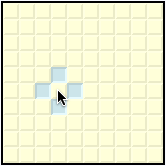
\includegraphics[width=.8\linewidth]{GameBoard}}
%	\caption{The Lights Out game board. The user has just clicked the mouse as shown by the cursor.
%	\figlabel{gameBoard}}
%\end{wrapfigure}

\begin{figure}[ht]
	\vskip -\baselineskip
	\centerline{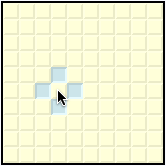
\includegraphics[width=.3\linewidth]{GameBoard}}
	\caption{El tablero del juego Lights Out. El usuario ha hecho clic con el rat\'on como muestra el cursor.
	\figlabel{gameBoard}}
\end{figure}


% To show you how to use \pharo's programming tools, we will build a simple game
% called \emph{Lights Out}.  The game board is shown in \figref{gameBoard}; it
% consists of rectangular array of light yellow \emph{cells}.  When you click on
% one of the cells with the mouse, the four surrounding cells turn blue.  \Click
% again, and they toggle back to light yellow.  The object of the game is to turn
% blue as many cells as possible.

Para mostrarle como utilizar las herramientas de \pharo, construiremos un un juego
sencillo llamado \emph{Lights Out}. El tablero del juego se muesta en \figref{gameBoard};
consiste en una grilla rectagular de \emph{celdas} amarillas. Cuando haces clic
sobre una celda con el rat\'on, las cuatro celdas adyacentes se tornan azules. Si
haces \Click otra vez, se volver\'an otras vez amarillas. El objetivo del juego
es poner azules la mayor cantidad de celdas como sea posible.

% The Lights Out game shown in \figref{gameBoard} is made up of two kinds of
% objects: the game board itself, and 100 individual cell objects.  The \pharo
% code to implement the game will contain two classes: one for the game and one
% for the cells.  We will now show you how to define these classes using the
% \pharo programming tools.

En el Lights Out que se muesta \figref{gameBoard} est\'a compuesto por
dos objetos: el tablero del juego en s\'i, y 100 objetos celda individuales. El
c\'odigo de \pharo para implementar el juego tendr\'a dos clases: una para el
juego y otra para las celdas. Ahora veremos c\'omo definir estas clases usando
las herramientas de programaci\'on de \pharo.

\section{Creando un paquete nuevo}

% We have already seen the \ind{browser} in \charef{quick}, where we learned how
% to navigate to classes and methods, and saw how to define new methods.  Now we
% will see how to create packages, categories and classes.

Ya hemos visto el \ind{Browser} en \charef{quick}, donde aprendimos como
navegar clases y m\'etodos, y vimos como definir nuevos m\'etodos. Ahora veremos
como crear paquetes, categor\'ias y clases.

\index{category!creating}
\index{package!creating}

% \dothis{Open a browser and \actclick in the package pane.  
% Select \menu{create package}.\footnote{We are assuming that the Package Browser is 
% installed as the default browser, which should normally 
% be the case. If the browser you get does
% not look like the one shown in \figref{addPackage}, then you may need to change
% the default browser.  See \faqref{packagebrowser}.}}

\dothis{Abre el explorador y seleccione la herramienta package.
Selecciona \menu{create package}.\footnote{Estamos asumiendo que el explorador
de paquetes est\'a instalado como el explorador por defecto, lo que
ocurre en casi todos los casos. Si el navagador que obtienes no se
ve similar al de \figref{addPackage}, entonces tal vez tengas que cambiar
el explorador por defecto. Mira \faqref{packagebrowser}.}}

\begin{figure}[htb]
\begin{minipage}[b]{0.48\textwidth}
\ifluluelse
	{\centerline {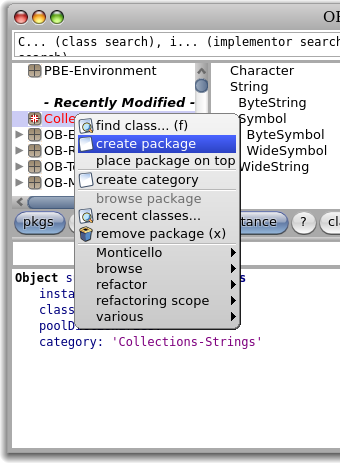
\includegraphics[width=0.9\textwidth]{AddPackage}}}
	{\centerline {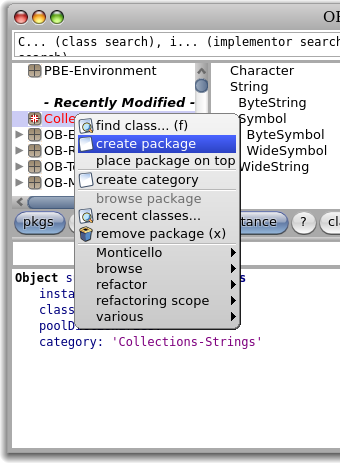
\includegraphics[scale=0.7]{AddPackage}}}
	\caption{Agregando un paquete.
	\figlabel{addPackage}}
\end{minipage}
\hfill
\begin{minipage}[b]{0.48\textwidth}
\ifluluelse
	{\centerline {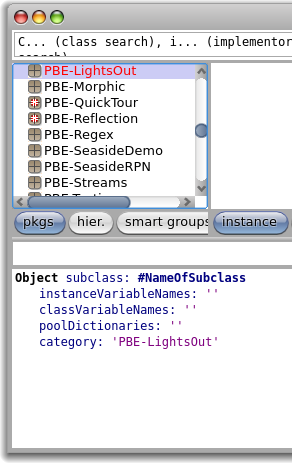
\includegraphics[width=0.8\textwidth]{ClassTemplate}}}
	{\centerline {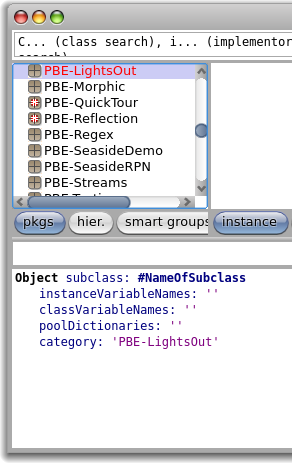
\includegraphics[scale=0.6]{ClassTemplate}}}
	\caption{La plantilla de una clase.
	\figlabel{classTemplate}}
\end{minipage}
\end{figure}

% Type the name of the new package (we will use \scat{PBE-LightsOut}) in the
% dialog box and click \menu{accept} (or just press the return key); the new
% package is created, and positioned alphabetically in the list of packages.

Escribe el nombre del nuevo paquete (usaremos \scat{PBE-LightsOut}) en
el cuadro de di\'alogo y selecciona \menu{accept} (o solo pulsa
la tecla enter); El nuevo paquete se ha creado, y se posiciona alfabeticamente
en la lista de paquetes.

%=================================================================
% \section{Defining the class LOCell}
\section{Definiendo la clase LOCell}

% As yet there are  of course no classes in the new package. However, the main
% editing pane displays a template to make it easy to create a new class (see
% \figref{classTemplate}).

Por supuesto, todav\'ia no hay clases en el nuevo paquete. A\'un as\'i, el panel
principal de edici\'on nos muestra una plantilla para hacer m\'as sencilla la tarea de crear
una nueva clase (ver \figref{classTemplate}).



% This template shows us a \st expression that sends a message to a class called
% \ct{Object}, asking it to create a subclass called \ct{NameOfSubClass}.  The
% new class has no variables, and should belong to the category
% \scat{PBE-LightsOut}.

Esta plantilla nos muestra una \st expression que env\'ia un mensaje a la clases
que se llama \ct{Object}, solicit\'andole que genere una subclase llamada
\ct{NameOfSubClass}. La nueva clase no tendr\'a variables, y deber\'a pertenecer
a la categor\'ia \scat{PBE-LightsOut}.

% \subsection{On Categories and Packages}
\subsection{Sobre categor\'ias y paquetes}
\seclabel{categoriesPackages}

% Historically, \st only knows about \emph{categories}, not packages.
% You may well ask, what is the difference?
% A category is simply a collection of related classes in a \st image.
% A \emph{package} is a collection of related classes \emph{and extension methods} that may be versioned using the Monticello versioning tool.
% By convention, package names and category names are the same.
% For most purposes we do not care about the difference, but we will be careful to use the correct terminology in this book since there are points where the difference is crucial.
% We will learn more when we start working with Monticello.
% \index{package}
% \index{category}

Hist\'oricamente, se trata sobre \emph{categor\'ias}, no paquetes.
Entonces podr\'ias preguntarte, ?`cual es la diferencia?
Una categor\'ia es simplemente una colecci\'on de clases relacionanadas en
una \st im\'agen.
Un \emph{paquete} es una colecci\'on de clases relacionadas junto a
\emph{m\'etodos de extensi\'on} que podr\'ian estar bajo un control de versiones
como Monticello.
Por convenci\'on, los nombres de paquetes y categor\'ias son siempre los mismos.
En la mayor\'ia de los casos no nos preocuparemos por las diferencias, pero
seremos cuidadosos en la terminolog\'ia de este libro para utilizar la
denominaci\'on correcta, ya que hay puntos donde de la diferencia es crucial.
Aprenderemos m\'as sobre este tema cuando comencemos a trabajar con Monticello.
\index{package}
\index{category}


% \subsection{Creating a new class}
\subsection{Creating a new class}

Solamente modificaremos la plantilla para crear la clase que realmente queremos.

\dothis{Modifique la plantilla de creaci\'on de clase como sigue:}
\begin{itemize}
  \item Reemplace \clsind{Object} por \clsind{SimpleSwitchMorph}.
  \item Reemplace \ct{NameOfSubClass} por \clsind{LOCell}.
  \item Añada \ct{mouseAction} a la lista de variables de instancia.
\end{itemize}
El resultado deber\'ia parecerse a \clsref{firstClassDef}.

\needlines{5}
\begin{classdef}[firstClassDef]{Defining the class \ct| LOCell|}
SimpleSwitchMorph subclass: #LOCell
   instanceVariableNames: 'mouseAction'
   classVariableNames: ''
   poolDictionaries: ''
   category: 'PBE-LightsOut'
\end{classdef}
\index{browser!defining a class}
\index{class!creation}
\index{Morphic}

% This new definition consists of a \st expression that sends a message to the
% existing class \ct{SimpleSwitchMorph}, asking it to create a subclass called
% \ct{LOCell}.  (Actually, since \ct{LOCell} does not exist yet, we passed as an
% argument the \emphind{symbol} \ct{#LOCell} which stands for the name of the
% class to create.) We also tell it that instances of the new class should have a
% \ct{mouseAction} instance variable, which we will use to define what action the
% cell should take if the mouse should click over it.

Esta nueva definici\'on consiste de una expresi\'on \st que env\'ia un mensaje a la
clase existente \ct{SimpleSwitchMorph}, pidi\'endole que cree una subclase llamada
\ct{LOCell}. (En realidad, como \ct{LOCell} no existe a\'un, se le pasa 
\emphind{symbol} \ct{#LOCell} como argumento, que indica el nombre de la clase a 
crear). Tambi\'en le indicamos que las instancias de la nueva clase deber\'ian 
tener una instancia de variable de \ct{mouseAction}, que usaremos para definir
que acci\'on deber\'ia tomar la celda si se hiciera clic sobre esta.


% \emph{At this point you still have not created anything.}
% Note that the border of the class template pane has changed to red (\figref{acceptClassDef}).
% This means that there are \emph{unsaved changes}.
%WIP To actually send this message, you must \menu{accept} it.

\emph {Hasta el momento no has creado nada.}
Nota que el borde del panel de template de clase cambi\'o a rojo (\figref{acceptClassDef}).
Esto significa que hay cambios \emph {sin guardar.}
Para enviar este mensaje, debes seleccionar \menu {accept}. 



%WIP \begin{figure}[h!t]
%WIP \ifluluelse
%WIP	 {\centerline {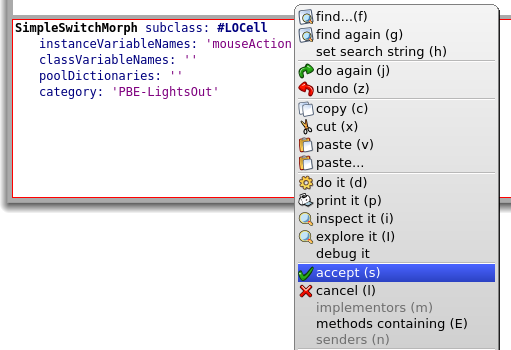
\includegraphics[width=\textwidth]{AcceptClassDef}}}
%WIP	 {\centerline {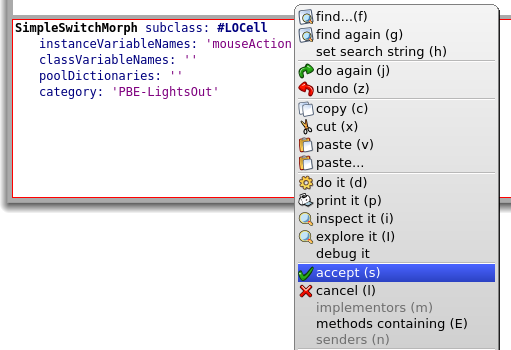
\includegraphics[scale=0.7]{AcceptClassDef}}}
%WIP \caption{The class-creation Template.
%WIP \figlabel{acceptClassDef}}
%WIP \end{figure}

\begin{figure}[h!t]
\ifluluelse
  {\centerline {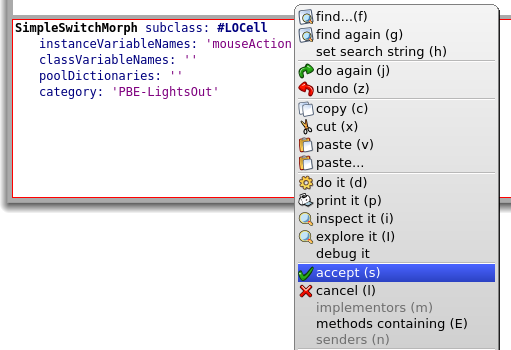
\includegraphics[width=\textwidth]{AcceptClassDef}}}
  {\centerline {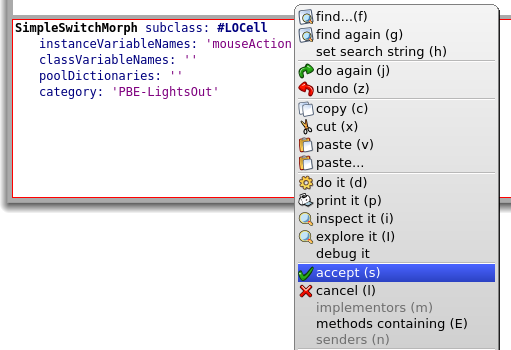
\includegraphics[scale=0.7]{AcceptClassDef}}}
\caption{Template de creaci\'on de clase.
\figlabel{acceptClassDef}}
\end{figure}

% \dothis{Accept the new class definition.}
% Either \actclick and select \menu{accept}, or use the shortcut \short{s} (for ``save'').
% The message will be sent to \ct{SimpleSwitchMorph}, which will cause the new class to be compiled.
% \index{keyboard shortcut!accept}

\dothis{Aceptar la definici\'on de la nueva clase.}
Esto se puede hacer de dos formas: o bien \actclick y selecciona \menu{accept}, o bien
usa el atajo \short{s} (para ``guardar'').
El mensaje ser\'a enviado a \ct{SimpleSwitchMorph}, causando que la nueva clase sea compilada.
\index{keyboard shortcut!accept} % <-- ver si hay que traducir esto.

% Once the class definition is accepted, the class will be created and appear in the classes pane of the browser (\figref{LOCell}).
% The editing pane now shows the class definition, and a small pane below it will remind you to write a few words describing the purpose of the class. This is called a \emph{class comment}, and it is quite important to write one that will give other programmers a high-level overview of the purpose of this class.
% Smalltalkers put a very high value on the readability of their code, and detailed comments in methods are unusual: the philosophy is that the code should speak for itself. (If it doesn't, you should refactor it until it does!) A class \subind{class}{comment} need not contain a detailed description of the class, but a few words describing its overall purpose are vital if programmers who come after you are to know whether to spend time looking at this class.
% \index{refactoring}

Una vez que la definici\'on de la clase es aceptada, la clase ser\'a creada y aparecer\'a en el panel de clases del navegador (\figref{LOCell}).
Ahora el panel de edici\'on muestra la definici\'on de la clase, y un pequeño panel debajo te recordar\'a escribir unas pocas palabras describiendo el prop\'osito de la clase. Esto se llama \emph {comentario de la clase}. Es importante escribir un comentario que le de a otros programadores una visi\'on de alto nivel del prop\'osito de la clase.
Los desarrolladores Smalltalk le dan un gran valor a la legibilidad de su c\'odigo, y es poco com\'un entcontrar comentarios detallados dentro de los m\'etodos: la filosof\'ia de Smalltalk es que el c\'odigo debe ser autoexplicativo. (Si no lo es, !`deber\'ias refactorizarlo hasta que lo sea!) Una clase \subind{clase}{comentario} no deber\'ia contener una descripci\'on detallada de la clase, pero unas pocas palabras que describan su prop\'osito de manera general son vitales para que otros programadores sepan si vale la pena invertir tiempo en mirar la clase o no.
\index{refactoring}

%\dothis{Type a class comment for \ct{LOCell} and accept it; you can always improve it later.}
\dothis{Escribe un comentario de clase para \ct{LOCell} y gu\'ardalo; siempre se puede mejorar m\'as tarde.}

\begin{figure}[h!t]
\ifluluelse
	{\centerline {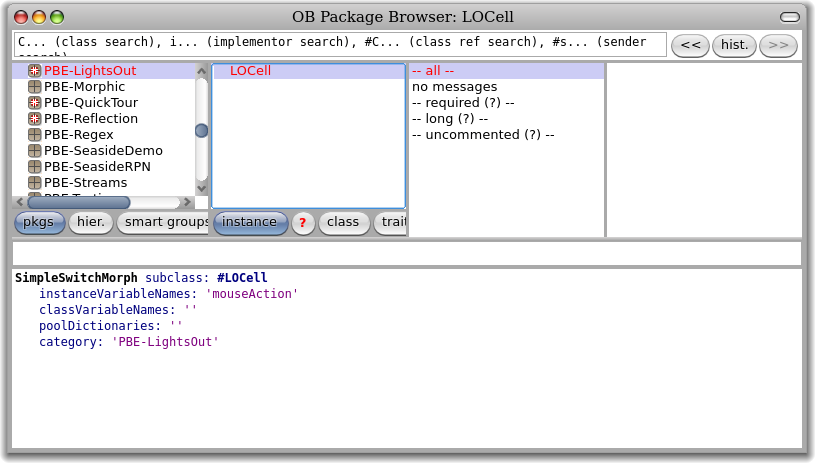
\includegraphics[width=\textwidth]{LOCell}}}
	{\centerline {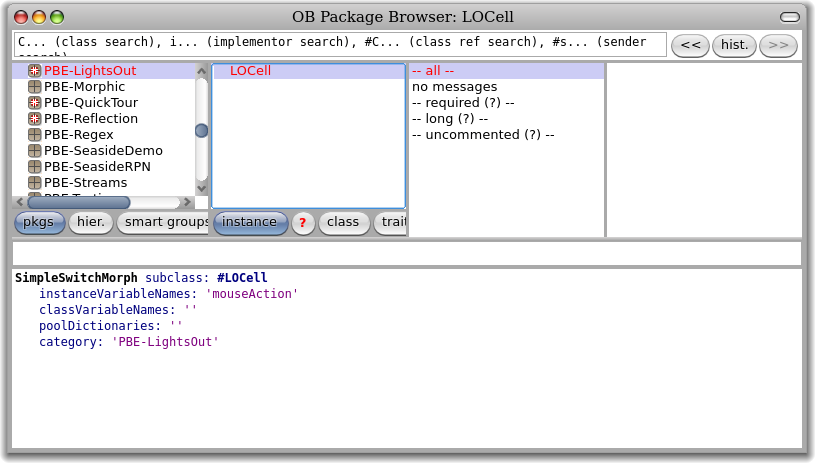
\includegraphics[scale=0.7]{LOCell}}}
\caption{La nueva clase creada \ct{LOCell}\figlabel{LOCell}}
\end{figure}


%=================================================================
%\section{Adding methods to a class}
\section{Agregando m\'etodos a una clase}

%Now let's add some methods to our class.
Ahora agreguemos algunos m\'etodos a nuestra clase.

% \dothis{Select the protocol \prot{-{}-all-{}-} in the protocol pane.}
% You will see a template for method creation in the editing pane.
% Select it, and replace it by the text of \mthref{scbecellinitialize}.
% \protindex{all}
% \index{method!creation}
% \index{browser!defining a method}

\dothis{Selecciona el protocolo \prot{-{}-all-{}-} en el panel de protocolos.}
Ver\'as un template para la creaci\'on de m\'etodos en el panel de edici\'on.
Selecci\'onalo y reemplazalo por el texto de \mthref{scbecellinitialize}.
\protindex{all}
\index{method!creation}
\index{browser!defining a method}


\needlines{10}
\begin{numMethod}[scbecellinitialize]{Initializing instances of \ct{LOCell}}
initialize
   super initialize.
   self label: ''.
   self borderWidth: 2.
   bounds := 0@0 corner: 16@16.
   offColor := Color paleYellow.
   onColor := Color paleBlue darker.
   self useSquareCorners.
   self turnOff
\end{numMethod}
\index{initialization}

%\noindent
% Note that the characters \ct{''} on line 3 are two separate single quotes with nothing between them, not a double quote!  \ct{''} denotes the empty string.

\noindent
Notar que los caracteres \ct{''} en la l\'inea 3 son comillas simples sin nada en el medio, no una doble comilla. \ct{''} es una cadena de caracteres vac\'ia. 

%\dothis{\menu{Accept} this method definition.}

\dothis{\menu{Aceptar} la definici\'on de este m\'etodo.}

%What does the above code do?  We won't go into all of the details here (that's what the rest of the book is for!), but we will give you a quick preview.  Let's take it line by line.

?`Qu\'e hace el c\'odigo de arriba? No nos adentraremos en los detalles aqu\'i (para eso es el resto del libro!), pero te daremos una breve introducci\'on. Ve\'amoslo l\'inea por l\'inea.

%Notice that the method is called \mthind{LOCell}{initialize}.
%The name is very significant!
%By convention, if a class defines a method named \ct{initialize}, it will be called right after the object is created.
%So, when we evaluate \ct{LOCell new}, the message \ct{initialize} will be sent automatically to this newly created object.
%Initialize methods are used to set up the state of objects, typically to set their instance variables; this is exactly what we are doing here.
%\seeindex{Object!initialization}{initialization}
%\index{initialization}

Notar que el m\'etodo se llama \mthind{LOCell}{initialize}.
El nombre es muy significativo!
Por convenci\'on, si una clase define un m\'etodo llamado \ct{initialize}, este ser\'a llamado inmediatamente despu\'es que el objeto sea creado. 
Entonces, cuando evaluamos \ct{LOCell new}, el mensaje \ct{initialize} ser\'a enviado autom\'aticamente al objeto reci\'en creado. 
Los m\'etodos "initialize" se usan para establecer el estado de los objetos, normalmente para establecer las variables de instancia; esto es exactamente lo que estamos haciendo ac\'a. 
\seeindex{Object!initialization}{initialization}
\index{initialization}

% The first thing that this method does (line 2) is to execute the \ct{initialize} method of its superclass, \ct{SimpleSwitchMorph}.
% The idea here is that any inherited state will be properly initialized by the \ct{initialize} method of the superclass.
% It is always a good idea to initialize inherited state by sending \ct{super initialize} before doing anything else; we don't know exactly what \ct{SimpleSwitchMorph}'s \ct{initialize} method will do, and we don't care, but it's a fair bet that it will set up some instance variables to hold reasonable default values, so we had better call it, or we risk starting in an unclean state.

Lo primero que hace este m\'etodo (l\'inea 2) es ejecutar el m\'etodo \ct{initialize} de su superclase, \ct{SimpleSwitchMorph}.
% Superclass lo traducimos como superclase o como clase padre o como? <----
El objetivo de esto es que cualquier estado heredado sea inicializado adecuadamente por el m\'etodo \ct{initialize} de la superclase.
Siempre es buena idea inicializar estado heredado enviando el mensaje \ct{super initialize} antes de hacer cualquier otra cosa; no sabemos exactamente que har\'a el m\'etodo \ct{initialize} de \ct{SimpleSwitchMorph}, y no nos importa, pero seguramente inicializar\'a algunas variables de instancia para que contengan valores razonables, por lo que es mejor invocarlo para no arriesgarse a que los objetos empiecen en un estado inv\'alido.

% The rest of the method sets up the state of this object.
% Sending \ct{self label: ''}, for example, sets the label of this object to the empty string.
% \pvindex{self}

El resto del m\'etodo establece el estado del objeto.
Enviar el mensaje \ct{self label: ''}, por ejemplo, establece la etiqueta de este objeto a la cadena de caracteres vac\'ia.
\pvindex{self}

% The expression \ct{0@0 corner: 16@16} probably needs some explanation. 
% \lct{0@0} represents a \clsind{Point} object with $x$ and $y$ coordinates both set to 0.
% In fact, \ct{0@0} sends the message \ct{@}

La expresi\'on \ct{0@0 corner: 16@16} probablemente necesite un poco de explicaci\'on.
\lct{0@0} representa un objeto \clsind{Point} con las coordenadas $x$ e $y$ en 0.
De hecho, \ct{0@0} env\'ia el mensaje \ct{@}

% Yuck... the following should be \mthind{Number}{@} 
%%% THIS IS BROKEN -- don't do it! (on)
%\def\atsign{\textsf{@}}%
%{\makeatletter
%	\protected@write\@indexfile{}%
%    {\string\indexentry{\string\atsign|see{Number, \string\atsign}}{\thepage}}%
%	\protected@write\@indexfile{}%
%    {\string\indexentry{Number!\string\atsign|hyperpage}{\thepage}}%
%	\makeatother}

% to the number \ct{0} with argument \ct{0}.
% The effect will be that the number \ct{0} will ask the \ct{Point} class to create a new instance with coordinates (0,0).
% Now we send this newly created point the message \ct{corner: 16@16}, which causes it to create a \clsind{Rectangle} with corners \ct{0@0} and \ct{16@16}.
% This newly created rectangle will be assigned to the \ct{bounds} variable, inherited from the superclass.

al n\'umero \ct{0} con par\'ametro \ct{0}.
El efecto ser\'a que el n\'umero \ct{0} le pedir\'a a la clase \ct{Point} que cree una nueva instancia con coordenadas (0,0).
Ahora le enviamos a este nuevo punto el mensaje \ct{corner: 16@16}, que hace que cree un \clsind{Rectangle} con esquinas \ct{0@0} y \ct{16@16}.
Este nuevo rect\'angulo ser\'a asignado a la variable \ct{bounds}, heredada de la superclase. 

% Note that the origin of the \pharo screen is the \emph{top left}, and the $y$ coordinate increases \emph{downwards}.
Nota que el or\'igen de la pantalla de \pharo es la \emph{esquina izquierda}, y la coordenada $y$ se incrementa hacia \emph{abajo}.

% The rest of the method should be self-explanatory.
% Part of the art of writing good \st code is to pick good method names so that \st code can be read like a kind of pidgin English.
% You should be able to imagine the object talking to itself and saying ``\ct{Self use square corners!}'', ``\ct{Self turn off!}''.

El resto del m\'etodo deber\'ia ser auto explicativo. 
Parte de arte de escribir buen c\'odigo \st es escoger los nombres adecuados para los m\'etodos para que el c\'odigo pueda ser leido como una especie de ingl\'es macarr\'onico. 
Deber\'ias poder imaginar al objeto hablandose a s\'i mismo y diciendo ``\ct{Self use square corners!}'', ``\ct{Self turn off}''.

%=================================================================
% \section{Inspecting an object}
\section{Inspeccionando un objeto}

% You can test the effect of the code you have written by creating a new \ct{LOCell} object and inspecting it.
Puedes probar el efecto del c\'odigo que acabas de escribir creando un nuevo objeto \ct{LOCell} y luego inspeccion\'andolo. 

% \dothis{Open a workspace. Type the expression \ct{LOCell new} and \menu{inspect it}.}
\dothis{Abre un workspace. Tipea la expresi\'on \ct{LOCell new} y \menu{inspect it}.}

%\begin{figure}[htbp]
%   \centering
%   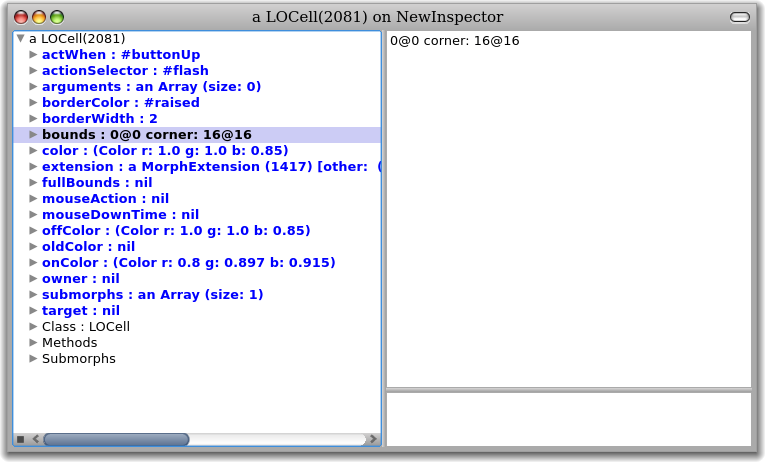
\includegraphics[width=\textwidth]{LOCellInspector} 
%   \caption{The inspector used to examine a LOCell object.\figlabel{LOCellInspector}}
%\end{figure}

\begin{figure}[htbp]
   \centering
   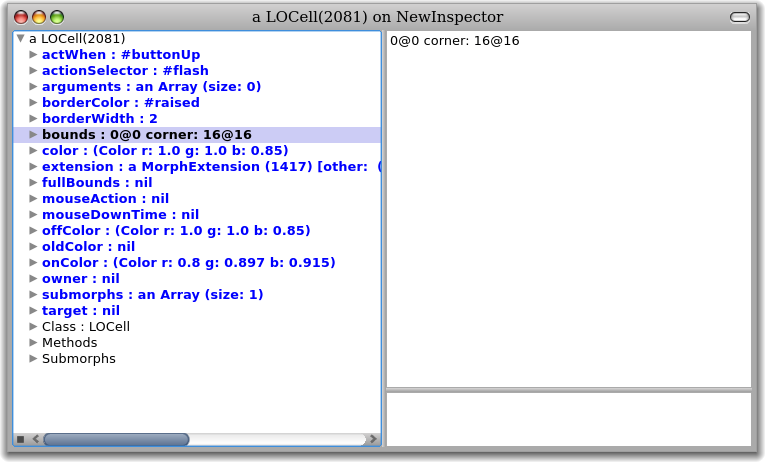
\includegraphics[width=\textwidth]{LOCellInspector} 
   \caption{El inspector usado para examinar un objeto LOCell.\figlabel{LOCellInspector}}
\end{figure}

% The left-hand pane of the \ind{inspector} shows a list of instance variables; if you select one (try \mbox{\ct{bounds}),} the value of the \ind{instance variable} is shown in the right pane.

El panel izquierdo de \ind{inpector} muestra una lista de variables de instancia; si seleccionas una (prueba \mbox{\ct{bounds}}), el valor de la \ind{variable de instancia} se muestra en el panel derecho. 

%--- Codigo que ya estaba comentado, no figura en la version original ---%
%  You can also use the inspector to change the value of an instance variable.
%\dothis{Change the value of \ct{bounds} to \ct{0@0 corner: 50@50} and \menu{accept} it.}
%\on{This does not work any more. I get:}
%\ct{OTNamedVariableNode(Object)>>doesNotUnderstand: #selectedClass}
%\on{should use the mini workspace instead to send bounds: ?}

% The bottom pane of the inspector is a mini-workspace.  It's useful because in this workspace the pseudo-variable \self is bound to the object selected. 
El panel inferior del inspector es un mini-workspace. Es muy \'util porque en este workspace la pseudo variable \self est\'a ligada al objeto seleccionado.

% \dothis{
% Select the LOCell at the root of the inspector window.
% Type the text \ct{self bounds: (200@200 corner: 250@250)} in the bottom pane and \menu{do it}. The \ct{bounds} variable should change in the inspector.
% Now type the text \ct{self openInWorld} in the mini-workspace and \menu{do it}.}
% The cell should appear near the top left-hand corner of the screen, indeed, exactly where its \ct{bounds} say that it should appear.
% \metaclick on the cell to bring up the morphic \subind{Morphic}{halo}.
% Move the cell with the brown (next to top-right) handle and resize it with the yellow (bottom-right) handle.
% Notice how the bounds reported by the inspector also change.
% (You may have to \actclick{} \menu{refresh} to see the new bounds value.)

\dothis{
Selecciona LOCell en la ra\'iz de la ventana del inspector.
Tipea el texto \ct{self openInWorld} en el mini-workspace y \menu{do it}.}
La celda deber\'ia aparecer cerca de la esquina superior izquierda de la pantalla, exactamente donde sus \ct{l\'imites} dicen que deber\'ia aparecer. 
\metaclick en la celda para que aparezca el halo de Morphic \subind{Morphic}. %% <---verificar
Mueve la celda con el asa marr\'on (esquina superior derecha) y redimensi\'onalo con el asa amarilla (abajo a la derecha).
Nota como los l\'imites reportados por el inspector tambi\'en cambian. 
(Tal vez tengas que \actclick{} \menu{refresh} para ver los nuevos valores de los l\'imites.)

% \begin{figure}[htbp]
% \centering
% \ifluluelse
% 	{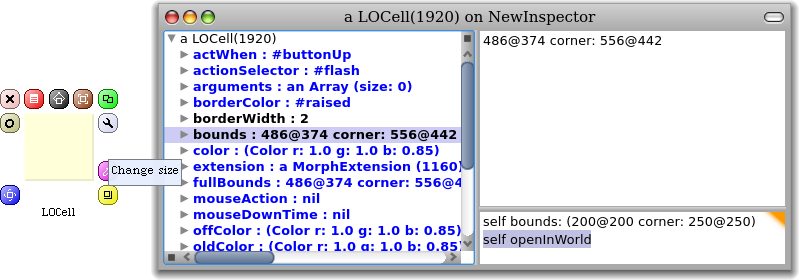
\includegraphics[width=\textwidth]{LOCellResize} }
% 	{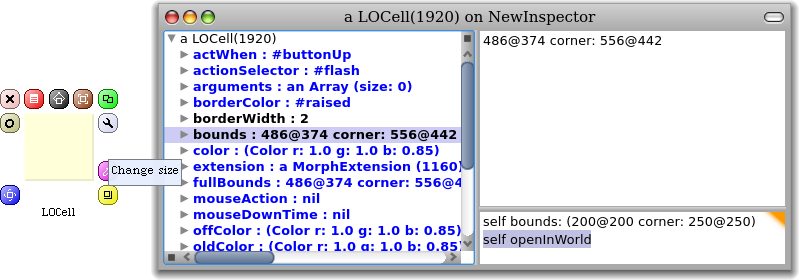
\includegraphics[scale=0.7]{LOCellResize} }
% \caption{Resizing the cell.\figlabel{cellresize}}
% \end{figure}

% \dothis{Delete the cell by clicking on the \ct{x} in the pink handle.}

\begin{figure}[htbp]
\centering
\ifluluelse
	{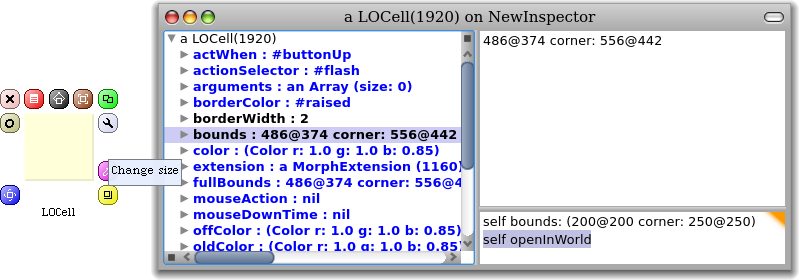
\includegraphics[width=\textwidth]{LOCellResize} }
	{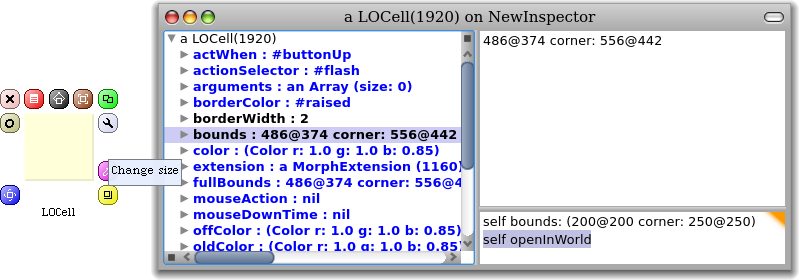
\includegraphics[scale=0.7]{LOCellResize} }
\caption{Redimensiona la celda.\figlabel{cellresize}}
\end{figure}

\dothis{Borra la celda haciendo clic en la \ct{x} en el asa rosa.}

%=================================================================
% \section{Defining the class LOGame}
\section{Definiendo la clase LOGame}

% Now let's create the other class that we need for the game, which we will call \clsind{LOGame}.
Ahora creemos la otra clase que necesitamos para el juego, que llamaremos \clsind{LOGame}.

% \dothis{Make the class definition template visible in the browser main window.}
% Do this by clicking on the package name.
% Edit the code so that it reads as follows, and \menu{accept} it.

\dothis{Has visible el template de definici\'on de clases en la ventana principal del navegador.}
Has esto haciendo clic en el nombre del paquete.
Edita el c\'odigo para que quede como se muestra a continuaci\'on, y has \menu{accept}.

\needlines{6}
\begin{classdef}[sbegame]{Defining the \ct{LOGame} class}
BorderedMorph subclass: #LOGame
   instanceVariableNames: ''
   classVariableNames: ''
   poolDictionaries: ''
   category: 'PBE-LightsOut'
\end{classdef}

% Here we subclass \clsind{BorderedMorph}; \clsind{Morph} is the superclass of all of the graphical shapes in \pharo, and (surprise!) a \ct{BorderedMorph} is a \ct{Morph} with a border.  
% We could also insert the names of the instance variables between the quotes on the second line, but for now, let's just leave that list empty.

Aqu\'i creamos una subclase de \clsind{BorderedMorph}; \clsind{Morph} es la superclase de todas las formas gr\'aficas e \pharo, y(sorpresa!) un \ct{BorderedMorph} es un \ct{Morph} con borde.
Podr\'iamos insertar los nombres de las variables de instancia entre comillas en la segunda l\'inea pero, por ahora, dejemos esa lista vac\'ia.

% Now let's define an \mthind{LOGame}{initialize} method for \ct{LOGame}.
Ahora definamos un m\'etodo \mthind{LOGame}{initialize} para \ct{LOGame}.

% \dothis{Type the following into the browser as a method for \ct{LOGame} and try to \menu{accept} it:}
\dothis{Escribe lo siguiente en el navegador como un m\'etodo para \ct{LOGame} e intenta \menu{accept}:}

\begin{numMethod}[sbegameinitialize]{Initializing the game}
initialize
   | sampleCell width height n |
   super initialize.
   n := self cellsPerSide.
   sampleCell := LOCell new.
   width := sampleCell width.
   height := sampleCell height.
   self bounds: (5@5 extent: ((width*n) @(height*n)) + (2 * self borderWidth)).
   cells := Matrix new: n tabulate: [ :i :j | self newCellAt: i at: j ].
\end{numMethod}

%\sd{it would be nicer if we would not have to create an instance of LOCell for nothing}
%\on{yes}

% \pharo will complain that it doesn't know the meaning of some of the terms.
% \pharo tells you that it doesn't know of a message \ct{cellsPerSide}, and suggests a number of corrections, in case it was a spelling mistake.

\pharo se quejar\'a de que no conoce el significado de ciertos t\'erminos.
\pharo dice que no conoce un mensaje \ct{cellsPerSide}, y sugiere algunas correcciones, en caso de que haya sido un error de tipeo.

\begin{figure}[htb]
\begin{minipage}{0.48\textwidth}
	\centering
	\ifluluelse
		{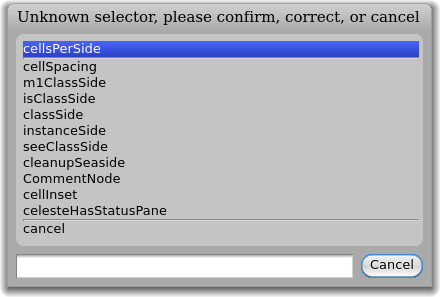
\includegraphics[width=\textwidth]{UnknownSelector}}
		{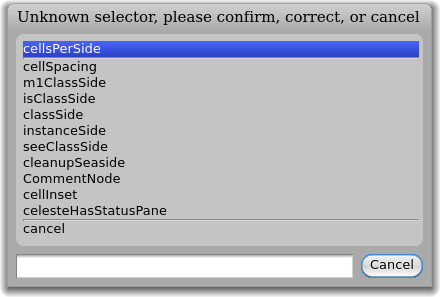
\includegraphics[scale=0.7]{UnknownSelector}}
%	\caption{\pharo detecting an unknown selector.\figlabel{unknownSelector}}
 \caption{\pharo detectando un identificador desconocido.\figlabel{unknownSelector}}
\end{minipage}
\hfill
\begin{minipage}{0.48\textwidth}
	\centering
	\ifluluelse
		{\includegraphics[width=\textwidth]{DeclareInstanceVar}}
		{\includegraphics[scale=0.7]{DeclareInstanceVar}}
%	\caption{Declaring a new instance variable.\figlabel{declareInstance}}
	\caption{Declarando una nueva variable de instancia.\figlabel{declareInstance}}
\end{minipage}
\end{figure}

% But \ct{cellsPerSide} is not a mistake\,---\,it is just a method that we haven't yet defined\,---\,we will do so in a minute or two.
Pero \ct{cellsPerSide} no es un error\,---\, es solo un m\'etodo que no hemos definido aun\,---\, lo haremos en un momento.

% \dothis{So just select the first item from the menu, which confirms that we really meant \ct{cellsPerSide}.}
\dothis{Selecciona el primer item del men\'u, que confirma que quisimos escribir \ct{cellsPerSide}.}

% Next, \pharo will complain that it doesn't know the meaning of \ct{cells}.  It offers you a number of ways of fixing this.
A continuaci\'on, \pharo se quejar\'a de que no conoce el significado de \ct{cells}. Te ofrece un n\'umero de formas de arreglar esto. 

% \dothis{Choose \menu{declare instance} because we want \ct{cells} to be an instance variable.}
% Finally, \pharo will complain about the message \ct{newCellAt:at:} sent on the last line; this is also not a mistake, so confirm that message too.
% \index{on the fly variable definition}
% \index{instance variable definition} 

\dothis{Elige \menu{declare instance} porque queremos que \ct{cells} sea una variable de instancia.}
Finalmente, \pharo se quejar\'a del mensaje \ct{newCellAt:at:} en la \'ultima l\'inea; esto tampoco es un error, asi que debes confirmar ese mensaje tambi\'en.
\index{on the fly variable definition}
\index{instance variable definition} 

% If you now look at the class definition once again (which you can do by clicking on the \button{instance} button), you will see that the browser has modified it to include the instance variable \ct{cells}.

Si miras ahora a la definici\'on de la clase de nuevo (cosa que puedes hacer haciendo clic en el bot\'on \button{nstance}), ver\'as que el navegador la modific\'o para incluir la variable de instancia \ct{cells}.

% Let's look at this \ct{initialize} method.
% The line \ct{| sampleCell width height n |}  declares 4 temporary variables. They are called temporary variables because their scope and lifetime are limited to this method.  Temporary variables with explanatory names are helpful in making code more readable.  Smalltalk has no special syntax to distinguish constants and variables, and in fact all four of these ``variables'' are really constants. 
% Lines 4--7 define these constants.
Miremos ahora al m\'etodo \ct{initialize}.
La l\'inea \ct{| sampleCell width height n |} declara 4 variables temporales. Son llamadas temporarias porque su \'ambito y tiempo de vida son limitados a este m\'etodo. Las variables temporales con nombres explicativos ayudan a hacer el c\'odigo m\'as legible. SMalltalk no tiene sintaxis especial para distinguir constantes y variables, y en realidad estas cuatro ``variables'' son en realidad constantes.
Las l\'ineas 4--7 definen estas constantes.

% How big should our game board be?  Big enough to hold some integral number of cells, and big enough to draw a border around them.
% How many cells is the right number?  5? 10? 100? We don't know yet, and if we did, we would probably change our minds later.  So we delegate the responsibility for knowing that number to another method, which we will call \ct{cellsPerSide}, and which we will write in a minute or two.
% It's because we are sending the \ct{cellsPerSide} message before we define a method with that name that \pharo asked us to ``confirm, correct, or cancel'' when we accepted the method body for \ct{initialize}.
% Don't be put off by this: it is actually good practice to write in terms of other methods that we haven't yet defined.
% Why?  Well, it wasn't until we started writing the \ct{initialize} method that we realized that we needed it, and at that point, we can give it a meaningful name, and move on, without interrupting our flow.
?`Qu\'e tan grande deber\'ia ser nuestro tablero de juego? Lo suficientemente grande como para almacenar algun n\'umero entero de celdas, y lo suficientemente grande como para dibujar un borde alrededor de ellas.
?`Cu\'al ser\'ia el n\'umero correcto de celdas? ?`5? ?`10? ?`100? No sabemos a\'un, y si supi\'eramos, probablemente cambiar\'iamos de parecer luego. As\'i que delegamos la responsabilidad de saber ese n\'umero a otro m\'etodo, que llamaremos \ct{cellsPerSide}, y que escribiremos en un momento.
Es porque estamos enviando el mensaje \ct{cellsPerSide} antes de definirlo que \pharo nos pidi\'o ``confirmar, corregir o cancelar'' cuando aceptamos el cuerpo del m\'etodo \ct{initialize}.
No te desanimes por esto: es en realidad una buena pr\'actica escribir en t\'erminos de m\'etodos que no hemos definido a\'un.
?`Por que? No fu\'e hasta que empezamos a escribir el m\'etodo \ct{initialize} que nos dimos cuenta que lo necesit\'abamos, y en ese momento, podemos darle un nombre significativo, y seguir adelante, sin interrumpir el flujo.
 
% The fourth line uses this method: 
% the Smalltalk \ct{self cellsPerSide} sends the message \ct{cellsPerSide} to \pvind{self}, i.e., to this very object.  
% The response, which will be the number of cells per side of the game board, is assigned to \ct{n}.
La cuarta l\'inea usa este m\'etodo:
El c\'odigo Smalltalk \ct{self cellsPerSide} env\'ia el mensaje \ct{cellsPerSide} a \pvind{self}, es decir, a este mismo objeto.
La respuesta, que ser\'a el n\'umero de celdas por lado del tablero de juego, es asignado a \ct{n}.

% The next three lines create a new \ct{LOCell} object, and assign its width and height to the appropriate temporary variables. 
Las siguientes tres l\'ineas crean un nuevo objeto \ct{LOCell}, y asignan su ancho y alto a las variables temporales adecuadas. 

%**** CODIGO COMENTADO EN LA VERSION ORIGINAL ****%
%The eighth line sends the message \ct{bounds:} to \self.
%\ct{bounds:} is a method that we inherit from our superclass; it is used to define the space on the screen that this Morph will occupy.  
%The single colon (\ct{:}) at the end of the name says that \ct{bounds:} expects a single parameter, which should be a rectangle object.
%**** FIN CODIGO COMENTADO ****%

% Line 8 sets the \ct{bounds} of the new object.
% Without worrying too much about the details just yet, just believe us that the expression in parentheses creates a square with its origin (\ie its top-left corner) at the point (5,5) and its bottom-right corner far enough away to allow space for the right number of cells.
La l\'inea 8 establece los \ct{l\'imites} del nuevo objeto.
Sin preocuparte mucho por los detalles ahora, conf\'ia en que la expresi\'on entre par\'entesis crea un cuadrado con or\'igen (\ie esquina superior izquierda) en el punto (5,5) y su esquina inferior derecha lo suficientemente lejos como para dar espacio al n\'umero correcto de celdas.

% The last line sets the \ct{LOGame} object's instance variable \ct{cells} to a newly created \clsind{Matrix} with the right number of rows and columns.   We do this by sending the message \ct{new:tabulate:} to the \ct{Matrix} class (classes are objects too, so we can send them messages).  We know that \mthind{Matrix class}{new:tabulate:} takes two arguments because it has two colons (\ct{:}) in its name.   The arguments go right after the colons.
% If you are used to languages that put all of the arguments together inside parentheses, this may seem weird at first.  Don't panic, it's only syntax!
% It turns out to be a very good syntax because the name of the method can be used to explain the roles of the arguments.  For example, it is pretty clear that \ct{Matrix rows: 5 columns: 2} has 5 rows and 2 columns, and not 2 rows and 5 columns.
% \cmindex{Matrix class}{rows:columns:}
La \'ultima l\'inea establece la variable de instancia \ct{cells} del el objeto \ct{LOGame} a una recien creada \clsind{Matrix} con el correcto n\'umero de filas y columnas. Hacemos esto enviando el mensaje \ct{new:tabulate:} a la clase \ct{Matrix} (las clases son objetos tambi\'en, por lo que les podemos enviar mensajes). Sabemos que \mthind{Matrix class}{new:tabulate} espera dos par\'ametros porque tiene dos s\'imbolos \ct{:} en su nombre. Los par\'ametros van justo despues de los s\'imbolos ':'.
Si est\'as acostumbrado a lenguajes que ponen todos los argumentos juntos dentro de par\'entesis, esto puede parecer raro al principio. !`No entres en p\'anico, es solo sintaxis!
Resulta que es una muy buena sintaxis porque el nombre de un m\'etodo puede ser usado para explicar los roles de los argumentos. Por ejemplo, es bastante claro que \ct{Matrix rows: 5 columns: 2} tiene 5 filas y 2 columnas, y no 2 filas y 5 columnas. 

\cmindex{Matrix class}{rows:columns:}

% \ct{Matrix new: n tabulate: [ :i :j | self newCellAt: i at: j ]} creates a new \ct{n}{$\times$}\ct{n} matrix and initializes its elements.  The initial value of each element will depend on its coordinates.  The \ct{(i,j)}\textsuperscript{th} element will be initialized to the result of evaluating \ct{self newCellAt: i at: j}.  
\ct{Matrix new: n tabulate: [ :i :j | self newCellAt: i at: j ]} crea una nueva matriz de \ct{n}{$\times$}\ct{n} e inicializa sus elementos. El valor inicial de cada elemento depender\'a de sus coordenadas.  El \ct{(i,j)}-\'esimo elemento ser\'a inicializado al resultado de evaluar \ct{self newCellAt: i at: j}.

%:===> Pretty-print is broken! (how to pretty-print?)

% \on{I think it is silly to copy paste from the pretty-print view to the normal view}

%**** CODIGO COMENTADO EN LA VERSION ORIGINAL ****%
%That's \ct{initialize}.  When you accept this message body, you might want to take the opportunity to pretty-up the formatting.  You don't have to do this by hand: from the \actclick menu select \menu{more \ldots \go prettyprint}, and the browser will do it for you\damien{this didn't do anything to me}.  You have to \menu{accept} again after you have \subind{method}{pretty-print}{}ed a method, or of course you can \subind{keyboard shortcut}{cancel} 
%(\short{l}\,---\,that's a lower-case letter \emph{L}) if you don't like the result.
%Alternatively, you can set up the browser to use the pretty-printer automatically whenever it shows you code: use the the right-most button in the button bar to adjust the view.
%\seeindex{pretty-print}{method}

%If you find yourself using \menu{more\,\ldots} a lot, it's useful to know that you can hold down the {\sc shift} key when you click to directly bring up the \menu{more \ldots} menu.
%**** FIN CODIGO COMENTADO ****%

%=================================================================
% \section{Organizing methods into protocols}
\section{Organizando m\'etodos en protocolos}

% Before we define any more methods, let's take a quick look at the third pane at the top of the browser.
% In the same way that the first pane of the browser lets us categorize classes into packages so we are not overwhelmed by a very long list of class names in the second pane, so the third pane lets us categorize methods so that we are not overwhelmed by a very long list of method names in the fourth pane.   
% These categories of methods are called ``protocols''.
% \index{protocol}
Antes de definir m\'as m\'etodos, demos una r\'apida mirada al tercer panel en la parte superior del navegador. 
De la misma manera que el primer panel del navegador nos permite categorizar clases en paquetes para que no nos sintamos abrumados por una larga lista de nombres de clases en el segundo panel, el tercer panel nos permite categorizar m\'etodos para que no nos sintamos abrumados por una larga lista de nombres de m\'etodos en el cuarto panel.
Estas categor\'ias de m\'etodos se llaman ``protocolos''.
\index{protocolo}

% If there are only a few methods in a class, the extra level of hierarchy provided by protocols is not really necessary.
% This is why the browser also offers us the \prot{-{}-all-{}-} virtual protocol, which, you will not be surprised to learn, contains all of the methods in the class.
% \protindex{all}
Si s\'olo hay unos pocos m\'etodos en la clase, el nivel extra de jerarqu\'ia provisto por los protocolos no es realmente necesario.
Esta es la raz\'on por la que el navegador tambi\'en nos ofrece el protocolo virtual \prot{-{}-all-{}-}, que, como no te sorprender\'a, contiene todos los m\'etodos de la clase.
\protindex{all}

\begin{figure}[htbp]
   \centering
   \includegraphics[width=\textwidth]{Categorize} 
   %\caption{Automatically categorize all uncategorized methods.\figlabel{categorize}}
   \caption{Catergoriza autim\'aticamente todos los m\'etodos sin categorizar.\figlabel{categorize}}
\end{figure}

% If you have followed along with this example, the third pane may well contain the protocol \protind{as yet unclassified}.
Si has seguido este ejemplo, el tercer panel bien podr\'ia contener el protocolo \protind{as yet unclassified}.

% \dothis{\Actclick in the protocol pane and select \menu{various \go categorize automatically} to fix this, and move the \ct{initialize} methods to a new protocol called \protind{initialization}.}
% How does \pharo{} know that this is the right protocol?  Well, in general \pharo{} can't know, but in this case there is also an \ct{initialize} method in a superclass, and \pharo assumes that our \ct{initialize} method should go in the same category as the one that it overrides.
% \index{method!categorize}
\dothis{\Actclick en el panel de protocolo y selecciona \menu{various \go categorize automatically} para arreglar esto, y mueve los m\'etodos \ct{initialize} a un nuevo protocolo llamado \protind{initialization}.}
?`Como sabe \pharo que este es el protocolo correcto? Bueno, en general  \pharo{} no puede saberlo, pero en este caso tambi\'en hay un m\'etodo \ct{initialize} en una superclase, y \pharo asume que nuestro m\'etodo \ct{initialize} deber\'ia ir en la misma categor\'ia que el que est\'a sobreescribiendo. 
\index{method!categorize}

%*** CODIGO COMENTADO EN LA VERSION ORIGINAL ***%
%You may find that \pharo has already put your \ct{initialize} method into the \protind{initialization} protocol.
%If so, it's probably because you have loaded a package called \ct{AutomaticMethodCategorizer} into your image.
%*** FIN CODIGO COMENTADO EN LA VERSION ORIGINAL ***%

% \paragraph{A typographic convention.} Smalltalkers frequently use the notation ``\verb|>>|'' to identify the class to which a method belongs, so, for example, the \ct{cellsPerSide} method in class \ct{LOGame} would be referred to as \ct{LOGame>>cellsPerSide}.
% To indicate that this is \emph{not} \st syntax, we will use the special symbol \ct{>>>} instead, so this method will appear in the text as \ct{LOGame>>>cellsPerSide}
% \cmindex{Behavior}{>>}
\paragraph{Convenci\'on tipogr\'afica.} Los programadors Smalltalk usan con frecuencia la notaci\'on ``\verb|>>|'' para identificar la clase a la que pertenece un m\'etodo. Por ejemplo, el m\'etodo \ct{cellsPerSide} en la clase \ct{LOGame} ser\'ia referenciado como \ct{LOGame>>cellsPerSide}.
Para indicar que esto \emph{no es} sintaxis \st, usaremos en su lugar el s\'imbolo especial \ct{>>>}, con lo que el m\'etodo en el texto aparecer\'a como \ct{LOGame>>>cellsPerSide}.
\cmindex{Behavior}{>>}

% From now on, when we show a method in this book, we will write the name of the method in this form.  Of course, when you actually type the code into the browser, you don't have to type the class name or the \ct{>>>}; instead, you just make sure that the appropriate class is selected in the class pane.  
De ahora en adelante, cuando mostremos un m\'etodo en este libro, escribiremos el nombre del m\'etodo en esta forma. Por supuesto, cuando escribas el c\'odigo en el navegador, no tendr\'as que escribir el nombre del a clase ni \ct{>>>}; solo aseg\'urate de que la clase correcta est\'a seleccionada en el panel de clases. 


% Now let's define the other two methods that are used by the \ct{LOGame>>>initialize} method. Both of them can go in the \prot{initialization} protocol.
Ahora definamos los otros dos m\'etodos que son usados por el m\'etodo \ct{LOGame>>>initialize}. Ambos pueden ir dentro del protocolo \prot{initialization}.

% \begin{method}[sbegamecellsperside]{A constant method.}
\begin{method}[sbegamecellsperside]{Un m\'etodo constante.}
LOGame>>>cellsPerSide
   %"The number of cells along each side of the game"
   "El n\'umero de celdas a cada lado del juego"
   ^ 10
\end{method}
\cmindex{LOGame}{cellsPerSide}
\index{constant methods}

% This method could hardly be simpler: it answers the constant 10.  One advantage of representing constants as methods is that if the program evolves so that the constant then depends on some other features, the method can be changed to calculate this value.
Este m\'etodo no podr\'ia ser m\'as simple: responde con la constante 10. Una ventaja de representar constantes con m\'etodos es que si el programa evoluciona de manera que la constante depende de otras caracter\'isticas, el m\'etodo puede ser cambiado para calcular el nuevo valor. 

\needlines{10}
%\begin{method}[newCellAt:at:]{An initialization helper method}
\begin{method}[newCellAt:at:]{Un m\'etodo de inicializaci\'on}
LOGame>>>newCellAt: i at: j
   % "Create a cell for position (i,j) and add it to my on-screen
   % representation at the appropriate screen position.  Answer the new cell"
   "Crea una celda para la posici'on (i,j) y la agrega a la representacion
   en la pantalla en la posici\'on adecuada de la pantalla. Devuelve la nueva celda"
   | c origin |
   c := LOCell new.
   origin := self innerBounds origin.
   self addMorph: c.
   c position: ((i - 1) * c width) @ ((j - 1) * c height) + origin.
   c mouseAction: [self toggleNeighboursOfCellAt: i at: j]
\end{method}
\cmindex{LOGame}{newCellAt:at:}
%   ^ c      "omit this final line to create a bug"

% \dothis{Add the methods \ct{LOGame>>>cellsPerSide} and \ct{LOGame>>>newCellAt:at:}.}
% Confirm the spelling of the new selectors \ct{toggleNeighboursOfCellAt:at:} and \ct{mouseAction:}.
\dothis{Agrega los m\'etodos \ct{LOGame>>>cellsPerSide} y \ct{LOGame>>>newCellAt:at:}.}
Confirma la pronunciaci\'on de los nuevos m\'etodos \ct{toggleNeighboursOfCellAt:at:} y \ct{mouseAction:}.

% \Mthref{newCellAt:at:} answers a new LOCell, specialized to position \ct{(i, j)} in the \clsind{Matrix} of cells.
% The last line defines the new cell's \ct{mouseAction} to be the \emph{block}
% \mbox{\lct{[self toggleNeighboursOfCellAt: i at: j ]}.}
% In effect, this defines the callback behaviour to perform when the mouse is clicked.
% The corresponding method also needs to be defined.
\Mthref{newCellAt:at:} devuelve una nueva LOCell, especializada en la posici\'on \ct{(i,j)} en la \clsind{Matriz} de celdas.
La \'ultima l\'inea define el \ct{mouseAction} de la nueva celda como el \emph{bloque}
\mbox{\lct{[self toggleNeighboursOfCellAt: i at: j ]}.}
En efecto, esto define el comportamiento callback cuando se hace clic con el rat\'on. 
El m\'etodo correspondiente tambi\'en tiene que ser definido. 

\begin{method}[toggleNeighboursOfCellAt:at:]{The callback method}
LOGame>>>toggleNeighboursOfCellAt: i at: j
   (i > 1) ifTrue: [ (cells at: i - 1 at: j ) toggleState].
   (i < self cellsPerSide) ifTrue: [ (cells at: i + 1 at: j) toggleState].
   (j > 1) ifTrue: [ (cells at: i  at: j - 1) toggleState].
   (j < self cellsPerSide) ifTrue: [ (cells at: i at: j + 1) toggleState].
\end{method}
\cmindex{LOGame}{toggleNeighboursOfCellAt:at:}

% \Mthref{toggleNeighboursOfCellAt:at:} toggles the state of the four cells to the north, south, west and east of cell (\ct{i}, \ct{j}).  The only complication is that the board is finite, so we have to make sure that a neighboring cell exists before we toggle its state.
\Mthref{toggleNeighboursOfCellAt:at:} cambia el estado de las cuatro celdas al norte, sur, este y oeste de una celda (\ct{i}, \ct{j}). La \'unica complicaci\'on es que el tablero es finito, por lo que tenemos que asegurarnos que las celdas vecinas existen antes que cambiemos su estado. 

% \dothis{Place this method in a new protocol called \prot{game logic}. (\Actclick in the protocol pane to add a new protocol.)}
% To move the method, you can simply click on its name and drag it to the newly-created protocol (\figref{dragMethod}).
\dothis{Coloca este m\'etodo en un nuevo protocolo llamado \prot{game logic}. (\Actclick en el panel de protocolo para agregar un nuevo protocolo.)}
Para mover el m\'etodo, puedes hacer clic en su nombre y arrastrarlo dentro del nuevo protocolo (\figref{dragMethod}).

\begin{figure}[htbp]
   \centering
   \ifluluelse
		{\includegraphics[width=\textwidth]{DragMethod} }
		{\includegraphics[scale=0.7]{DragMethod} }
   % \caption{Drag a method to a protocol.\figlabel{dragMethod}}
   \caption{Arrastra un m\'etodo a un protocolo.\figlabel{dragMethod}}
\end{figure}

% To complete the Lights Out game, we need to define two more methods in class \ct{LOCell} to handle mouse events.
Para completar el juego Lights Out, necesitamos definir dos m\'etodos m\'as en la clase \ct{LOCell} para manejar los eventos del rat\'on.
% \begin{method}[mouseAction:]{A typical setter method}
\begin{method}[mouseAction:]{Un m\'etodo setter t\'ipico}
LOCell>>>mouseAction: aBlock
   ^ mouseAction := aBlock
\end{method}
\cmindex{LOCell}{mouseAction:}

% \Mthref{mouseAction:} does nothing more than set the cell's \ct{mouseAction} variable to the argument, and then answers the new value.
\Mthref{mouseAction:} no hace nada m\'as que establecer la variable \ct{mouseAction} de la celda al argumento, y luego retorna el nuevo valor.

% Any method that \emph{changes} the value of an instance variable in this way is called a \emph{setter method}; a method that \emph{answers} the current value of an instance variable is called a \emph{getter method}.
Cualquier m\'etodo que \emph{cambie} el valor de una variable de instancia de esta manera se llama \emph{m\'etodo setter}; un m\'etodo que \emph{retorna} el valor actual de una variable de instancia se llama \emph{m\'etodo getter}.
\seeindex{setter method}{accessor}
\seeindex{getter method}{accessor}

% If you are used to getters and setters in other programming languages, you might expect these methods to be called \ct{setmouseAction} and \ct{getmouseAction}.
Si est\'as acostumbrado a los getters y setters en otros lenguajes, podr\'ias esperar que estos m\'etodos se  llamen \ct{setmouseAction} and \ct{getmouseAction}.
% The \st convention is different.
%A getter always has the same name as the variable it gets, and a setter is named similarly, but with a trailing ``\ct{:}'', hence \ct{mouseAction} and \ct{mouseAction:}.
La convenci\'on \st es diferente. 
Un getter siempre tiene el mismo nombre que la variable que devuelve, y un setter siempre es llamado de manera similar, pero con un ``\ct{:}'' al final, por lo que queda \ct{mouseAction} and \ct{mouseAction:}.

% Collectively, setters and getters are called  \emphind{accessor} methods, and by convention they should be placed in the \protind{accessing} protocol.
% In Smalltalk, \emph{all} instance variables are private to the object that owns them, so the only way for another object to read or write those variables in the Smalltalk language is through accessor methods like this one\footnote{In fact, the instance variables can be accessed in subclasses too.}.
Colectivamente, los setters y getters son llamados m\'etodos \emphind{de acceso}, y por convenci\'on deber\'ian ser colocados en el protocolo \protind{accessing}.
En Smalltalk, \emph{todas} las variables de instancia son privadas para el objeto que las posee, por lo que la \'unica manera de leer o escribir esas variables para otro objeto en el lenguaje Smalltalk es a trav\'es de los m\'etodos de acceso como este\footnote{En realidad, las variables de instancia tambi\'en pueden ser accedidas desde las subclases.}.

% \dothis{Go to the class \ct{LOCell}, define \ct{LOCell>>>mouseAction:} and put it in the \prot{accessing} protocol.}
\dothis{Ve a la clase \ct{LOCell}, define \ct{LOCell>>>mouseAction:} y ponlo en el protocolo \prot{accessing}.}

% Finally, we need to define a method \ct{mouseUp:}; this will be called automatically by the GUI framework if the mouse button is released while the mouse is over this cell on the screen.
Finalmente, necesitamos definir un m\'etodo \ct{mouseUp:}; este ser\'a llamado autom\'aticamente por el GUI framework  si el bot\'on del rat\'on es soltado cuando el rat\'on est\'a sobre la celda en la pantalla.

% \begin{method}[sbecellmouseup]{An event handler}
\begin{method}[sbecellmouseup]{Un manejador de eventos}
LOCell>>>mouseUp: anEvent
   mouseAction value
\end{method}
\cmindex{LOCell}{mouseUp:}

% \dothis{Add the method \ct{LOCell>>>mouseUp:} and then
%   \menu{categorize automatically} methods.}
% \index{method!categorize}
\dothis{Agrega el m\'etodo \ct{LOCell>>>mouseUp:} y luego
  \menu{categorize automatically} los m\'etodos.}
\index{method!categorize}

% What this method does is to send the message \ct{value} to the object stored in the instance variable \ct{mouseAction}. 
% Recall that in \ct{LOGame>>>newCellAt: i at: j} we assigned the following code fragment to \ct{mouseAction}:
Lo que hace este m\'etodo es enviar el mensaje \ct{value} al objeto almacenado en la variable de instancia \ct{mouseAction}.
Recuerda que en \ct{LOGame>>>newCellAt: i at: j} asignamos el siguiente fragmento de c\'odigo a \ct{mouseAction}:

\ct{[self toggleNeighboursOfCellAt: i at: j ]} 

\noindent
% Sending the \ct{value} message causes this code fragment to be evaluated, and consequently the state of the cells will toggle.
Enviar el mensaje \ct{value} provoca que este fragmento de c\'odigo sea evaluado, y consecuentemente el estado de las celdas cambiar\'a. 

%=================================================================
% \section{Let's try our code}
\section{Probemos nuestro c\'odigo}

% That's it: the Lights Out game is complete!
Eso es: el juego Lights Out est\'a completo!

% If you have followed all of the steps, you should be able to play the game, consisting of just 2 classes and 7 methods.
Si has seguido todos los pasos, deber\'ias poder jugar el juego, que consiste en solo 2 clases y 7 m\'etodos.

% \dothis{In a workspace, type \ct{LOGame new openInWorld} and \menu{do it}.}
\dothis{En un workspace, tipea \ct{LOGame new openInWorld} y \menu{do it}.}

% The game will open, and you should be able to click on the cells and see how it works.
El juego se abrir\'a, y deber\'ias poder hacer clic en las celdas y ver como funciona. 

% Well, so much for theory\ldots{}
% When you click on a cell, a \emphind{notifier} window called the \clsind{PreDebugWindow}window appears with an error message!
% As depicted in \figref{lightsOutError}, it says \ct{MessageNotUnderstood: LOGame>>>toggleState}.
Bueno, demasiada teor\'ia\ldots{}
Cuando haces clic en una celda, una ventana de \emphind{notificaci\'on} llamada ventana \clsind{PreDebugWindow} aparece con un mensaje de error!
Como se muestra en \figref{lightsOutError}, dice \ct{MessageNotUnderstood: LOGame>>>toggleState}.

\begin{figure}[ht]
\ifluluelse
	{\centerline{\includegraphics[width=\textwidth]{Error}}}
	{\centerline{\includegraphics[scale=0.7]{Error}}}
%\caption{There is a bug in our game when a cell is clicked!
\caption{'!Hay un bug en nuestro juego cuando se hace clic en nuestra celda!
\figlabel{lightsOutError}}
\end{figure}

\noindent
% What happened? To find out, let's use one of Smalltalk's more powerful tools: the \ind{debugger}.
'¿Qu\'e pas\'o? Para averiguarlo, usemos uno de las herramientas m\'as poderosas de Smalltalk: el \ind{debugger}.

% \dothis{Click on the \menu{debug} button in the notifer window.}
% The debugger will appear.
% In the upper part of the debugger window you can see the execution stack, showing all the active methods; selecting any one of them will show, in the middle pane, the Smalltalk code being executed in that method, with the part that triggered the error highlighted.
\dothis{Haz clic en el bot\'on \menu{debug} en la ventana de notificaci\'on.}
El debugger aparecer\'a.
En la parte superior de la ventana del debugger puedes ver la pila de ejecuci\'on, mostrando todos los m\'etodos activos; seleccionando alguno de ellos se mostrar\'a, en el panel del medio, el c\'odigo Smalltalk ejecut\'andose en ese m\'etodo, con la parte que dispar\'o el error resaltada. 

% \dothis{Click on the line labelled
% \ct{LOGame>>>toggleNeighboursOfCellAt:at:} (near the top).}
% The debugger will show you the \ind{execution context} within this method where the error occurred (\figref{debugToggle}).
\dothis{Has clic en la l\'inea etiquetada 
\ct{LOGame>>>toggleNeighboursOfCellAt:at:} (near the top).}
El debugger te mostrar\'a el \ind{contexto de ejecuci\'on} de este m\'etodo donde ocurri\'o el error (\figref{debugToggle}).

\begin{figure}[ht]
\ifluluelse
	{\centerline {\includegraphics[width=\textwidth]{Debugger}}}
	{\centerline {\includegraphics[scale=0.7]{Debugger}}}
% \caption{The debugger, with the method \ct{toggleNeighboursOfCell:at:}  selected.
\caption{El debugger, con el m\'etodo \ct{toggleNeighboursOfCell:at:}  seleccionado.
\figlabel{debugToggle}}
\end{figure}

% At the bottom of the debugger are two small inspector windows.  On the left, you can inspect the object that is the receiver of the message that caused the selected method to execute, so you can look here to see the values of the instance variables.
% On the right you can inspect an object that represents the currently executing method itself, so you can look here to see the values of the method's parameters and temporary variables.
En la parte inferior del debugger hay dos pequeñas ventanas de inspecci\'on. A la izquierda, puedes inspeccionar el objeto receptor del mensaje que caus\'o que el mensaje seleccionado se ejecute, asi que pudes mirar aqu\'i para ver los valores de las variables de instancia.
A la derecha puedes inspeccionar un objeto que representa el m\'etodo que se est\'a ejecutando, asi que puedes mirar aqu\'i para ver los valores de los par\'ametros del m\'etodo y las variables temporales.


% Using the debugger, you can execute code step by step, inspect objects in parameters and local variables, evaluate code just as you can in a workspace, and, most surprisingly to those used to other debuggers, change the code while it is being debugged! Some Smalltalkers program in the debugger almost all the time, rather than in the browser.  The advantage of this is that you see the method that you are writing as it will be executed, with real parameters in the actual execution context.
Usando el debugger, puedes ejecutar c\'odigo paso a paso, inspeccionar objetos en par\'ametros y variables locales, evaluar c\'odigo como lo puedes hacer en el workspace, y, m\'as sorprendente a\'un para los que est\'an acostumbrados a otros debuggers, '!cambiar el c\'odigo mientras est\'a siendo debuggeado! Algunos programadores Smalltalk programan en el debugger casi todo el tiempo, en lugar de usar el browser. La ventaja de esto es que puedes ver el m\'etodo que est\'as escribiendo como ser\'a ejecutado, con par\'ametros reales en el contexto de ejecuci\'on real.

% In this case we can see in the first line of the top panel that the \ct{toggleState} message has been sent to an instance of \ct{LOGame}, while it should clearly have been an instance of \lct{LOCell}.
% The problem is most likely with the initialization of the \ct{cells} matrix.
% Browsing the code of \cmind{LOGame}{initialize} shows that \ct{cells} is filled with the return values of \ct{newCellAt:at:}, but when we look at that method, we see that there is no return statement there!
% By default, a method returns \ct{self}, which in the case of \ct{newCellAt:at:} is indeed an instance of \ct{LOGame}.
% \index{method!returning self}
En este caso podemos ver en la primera l\'inea del panel superior que el mensaje \ct{toggleState} fu\'e enviado a una instancia de \ct{LOGame}, cuando, claramente, deber\'ia haber sido una instancia de \lct{LOCell}.
El problema est\'a seguramente con la inicializaci\'on de la matriz \ct{cells}.
Explorando el c\'odigo de \cmind{LOGame}{initialize} nos muestra que \ct{cells} se llena con el valor de retorno de \ct{newCellAt:at:}, pero cuand miramos ese m\'etodo, '!vemos que no hay sentencia de retorno!
Por defecto, un m\'etodo retorna \ct{self}, que en el caso de \ct{newCellAt:at:} es de hecho una instancia de \ct{LOGame}.
\index{method!returning self}

% \dothis{Close the debugger window.
% Add the expression ``\ct{^ c}'' to the end of the method \ct{LOGame>>>newCellAt:at:} so that it returns \ct{c}.
%-- Codigo comentado en la version original --%
% It should now look as shown in \mthref{newCellAt:at:nobug}.}
%-- Fin codigo comentado en la version original --%
% (See \mthref{newCellAt:at:nobug}.)}

\dothis{Cierra la ventana del debugger.
Agrega la expresi\'on ``\ct{^ c}'' al final del m\'etodo \ct{LOGame>>>newCellAt:at:} para que devuelva \ct{c}.
(Ver \mthref{newCellAt:at:nobug}.)}

% \needlines{6}
\begin{method}[newCellAt:at:nobug]{Fixing the bug.}
LOGame>>>newCellAt: i at: j
   "Create a cell for position (i,j) and add it to my on-screen
   representation at the appropriate screen position.  Answer the new cell"
   | c origin |
   c := LOCell new.
   origin := self innerBounds origin.
   self addMorph: c.
   c position: ((i - 1) * c width) @ ((j - 1) * c height) + origin.
   c mouseAction: [self toggleNeighboursOfCellAt: i at: j].
   ^ c
\end{method}
\cmindex{LOGame}{newCellAt:at:}

% \noindent
%Recall from \charef{quick} that the construct to \ind{return} a \subind{method}{value} from a method in Smalltalk is \ct{^}, which you obtain by typing \verb|^|.
% \index{^@\verb|^|}
% \index{^@{$\uparrow$}|see{return}}
\noindent
Recuerda de \charef{quick} que la manera de hacer \ind{return} de un \subind{method}{valor} de un m\'etodo en Smalltalk es \ct{^}, que obtienes tipeando \verb|^|.
\index{^@{$\uparrow$}|see{return}}
% Verificar si esta bien esto del subind... como se puede traducir?

% Often, you can fix the code directly in the debugger window and click \menu{Proceed} to continue running the application.
% In our case, because the bug was in the initialization of an object, rather than in the method that failed, the easiest thing to do is to close the debugger window, destroy the running instance of the game (with the \subind{Morphic}{halo}), and create a new one.
A menudo puedes arreglar el c\'odigo directamente en la ventaba del debugger y hacer clic en \menu{Proceed} para continuar corriendo la aplicaci\'on.
En nuestro caso, como el bug estaba en la inicializaci\'on de un objeto, y no en el m\'etodo que fall\'o, lo m\'as f\'acil
es cerrar la ventana de debug, destruir la intancia del juego ejecut\'andose (con el \subind{Morphic}{halo}), y crear una nueva.

%Indeed, even in this case it would be possible to \menu{do} \ct{self initialize} and then \menu{Proceed} the \ct{toggleNeighboursOfCellAt:at:} method.
%\ab{St\'eph, did you try this?  It seems to me that it ought to work, but when I tried it, it messed up my image.}
% ON : It messed me up too!  Better not propose this.

\dothis{Do: \ct{LOGame new openInWorld} again.}

% Now the game should work properly ... or nearly so.  If we happen to move the mouse between clicking and releasing, then the cell the mouse is over will also be toggled.  This turns out to be behavior that we inherit from \ct{SimpleSwitchMorph}. We can fix this simply by overriding \ct{mouseMove:} to do nothing:
Ahora el juego deber\'ia funcionar correctamente... o casi. Si hacemos clic, y luego movemos el rat\'on antes de soltar el bot\'on, la celda sobre la que esta el rat\'o tambi\'en cambiar\'a. Resulta que esto es comportamiento que heredamos de \ct{SimpleSwitchMorph}. Podemos arreglar esto simplemente sobreescribiendo \ct{moseMove:} para que no haga nada:

% \needlines{6}
\begin{method}[mouseMove:]{Overriding mouse move actions.}
LOGame>>>mouseMove: anEvent
\end{method}

% Finally we are done!
!`Finalmente terminamos!

%\sd{It would be good to have a word about the debugger buttons into, step.... Or to have a separate chapter, we would use the material I wrote for my turtle book, please check it.}
%\on{I think that is too much for this chapter. It will come soon enough.}

%=================================================================
% \section{Saving and sharing Smalltalk code}
\section{Guardando y compartiendo c\'odigo Samalltalk}
\seclabel{Monticello}

% Now that you have the Lights Out game working, you probably want to save it somewhere so that you can share it with your friends. Of course, you can save your whole \pharo image, and show off your first program by running it, but your friends probably have their own code in their images, and don't want to give that up to use your image.
% What you need is a way of getting source code out of your \pharo image so that other programmers can bring it into theirs.
Ahora que tienes el juego Lights Out funcionando, probablemente quieras guardarlo en alg\'un lugar para poder compartirlo con tus amigos. Por supuesto, puedes guardar tu im\'agen de \pharo completa, y mostrar tu primer programa ejecut\'andola, pero tus amigos probablemente tengan su propio c\'odigo en sus im\'agenes, y no quieran renunciar a eso para usar tu im\'agen. 
Lo que necesitas es una manera de sacar tu c\'odigo fuente fuera de tu im\'agen \pharo para que otros programadores puedan introducirla en las suyas. 

% The simplest way of doing this is by \emph{filing out} the code.  The \actclick menu in the Package pane will give you the option to \menu{various \go{} file out} the whole of package \scat{PBE-LightsOut}.
% The resulting file is more or less human readable, but is really intended for computers, not humans.
% You can email this file to your friends, and they can file it into their own \pharo images using the file list browser.
La manera m\'as sencilla de hacer esto es haciendo \emph{filing out} a nuestro c\'odigo. El men\'u \actclick en el panel de Paquete te dar\'a la opci\'on \menu{various \go{} file out} de todo el paquete \scat{PBE-LightsOut}.
El archivo resultante es m\'as o menos humanamente legible, pero est\'a realmente pensado para computadoras, no humanos. 
Puedes enviar este archivo via email a tus amigos, y ellos pueden archivarlo dentro de sus propias im\'agenes \pharo, usando el explorador de archivos.
\seeindex{saving code}{categories}
\seeindex{category!filing out}{file, filing out}
\seeindex{class!filing out}{file, filing out}
\seeindex{method!filing out}{file, filing out}
\index{file!filing out}
%Ver si esto se traduce
%%%------------HASTA ACA LLEGUE---------------%%%

% \dothis{\Actclick on the \scat{PBE-LightsOut} package and \menu{various \go{} file out} the contents.}
% You should now find a file called ``PBE-LightsOut.st'' in the same folder on disk where your image is saved.
% Have a look at this file with a text editor.
\dothis{\Actclick en el paquete \scat{PBE-LightsOut} y has \menu{various \go{} file out} de los contenidos.}
Ahora deber\'ias encontrar un archivo llamado ``PBE-LightsOut.st'' en el mismo directorio del disco donde se encuentra tu im\'agen.
Da una mirada a este archivo con un editor de texto.

% \dothis{Open a fresh \pharo image and use the File Browser tool (\menu{Tools \ldots {\go} File Browser}) to \menu{file in} the PBE-LightsOut.st fileout.
% Verify that the game now works in the new image.}
\dothis{Abre una nueva im\'agen de \pharo y usa la herramienta File Browser (\menu{Tools \ldots {\go} File Browser}) para hacer \menu{file in} al PBE-LightsOut.st fileout.
Verifica que el juego ahora funciona en la nueva im\'agen.}
\seeindex{category!filing in}{file, filing in}
\seeindex{class!filing in}{file, filing in}
\seeindex{method!filing in}{file, filing in}
\index{file!filing in}

\begin{figure}[ht]
\centerline {\includegraphics[width=\textwidth]{FileIn}}
% \caption{Filing in \pharo source code.
\caption{Filing in c\'odigo fuente \pharo.
\figlabel{filein}}
\end{figure}

% \subsection{Monticello packages}
% Although fileouts are a convenient way of making a snapshot of the code you have written, they are decidedly ``old school''.
% Just as most open-source projects find it much more convenient to maintain their code in a repository using \ind{CVS}\footnote{\url{http://www.nongnu.org/cvs}} or \ind{Subversion}\footnote{\url{http://subversion.tigris.org}},
% so \pharo programmers find it more convenient to manage their code using \ind{Monticello} packages. 
% These packages are represented as files with names ending in \ct{.mcz}; they are actually zip-compressed bundles that contain the complete code of your \ind{package}.
\subsection{Paquetes Monticello}
Por m\'as que los fileouts son una manera conveniente de tomar una fotograf\'ia del c\'odigo que has escrito, son definitivamente de ``la vieja escuela''.
As\'i como muchos proyectos open-source hallan mucho m\'as conveniente mantener su c\'odigo en un repositorio usando \ind{CVS}\footnote{\url{http://www.nongnu.org/cvs}} o \ind{Subversion}\footnote{\url{http://subversion.tigris.org}}, los programadores \pharo encuentran m\'as conveniente manejar su c\'odigo usando paquetes \ind{Monticello}.
Estos paquetes se representan como archivos con nombres terminados en \ct{.mcz}; son en realidad paquetes comprimidos en formato zip que contienen el c\'odigo completo de tu \ind{paquete}.

% Using the Monticello package browser, you can save packages to repositories on various types of server, including FTP and HTTP servers; you can also just write the packages to a repository in a local file system directory.
% A copy of your package is also always cached on your local hard-disk in the \emph{package-cache} folder. 
% Monticello lets you save multiple versions of your program, merge versions, go back to an old version, and browse the differences between versions. 
Usando el navegador de paquetes Monticello, puedes guardar paquetes en repositorios en varios tipos de servidores, incluyendo servidores FTP y HTTP; tambi\'en puedes escribir paquetes en un repositorio en un sistema de archivos local. 
Una copia de tu paquete se cachea siempre en tu disco duro local, en el directorio \emph{package-cache}.
Monticello te permite guardar m\'ultiples versiones de tu programa, mezclar versiones, volver a una versi\'on vieja, y ver las diferencias entre las versiones.

% In fact, Monticello is a distributed revision control system; this means it allows developers to save their work on different places, not on a single repository as it is the case with CVS or Subversion.\damien{Mercurial, Git are examples of distributed revision control system; not sure it's worth mentioning them.}
% \seeindex{package browser}{Monticello}
De hecho, Monticello es un sistema de control de versiones distribuido; esto significa que permite a los desarrolladores guardar su trabajo en diferentes lugares, no en un solo repositorio como es el caso de CVS o Subversion. 
\seeindex{package browser}{Monticello}
 
% You can also send a \ct{.mcz} file by email. 
% The recipient will have to place it in her \emph{package-cache} folder; she will then be able to use Monticello to browse and load it. 
Tambi\'en puedes enviar un archivo \ct{.mcz} por email.
El receptor tendr\'a que ponerlo en su directorio \emph{package-cache}; Luego ser\'ra capaz de usar Monticello para navegar y cargarlo.
%(It is also possible to load it using the file list, but there is a difference between loading a \ct{.mcz} file using a file list and using Monticello \sd{check}.)


% \dothis{Open the Monticello browser from the \menu{World} menu.}
% In the right-hand pane of the browser (see \figref{monticello1}) is a list of Monticello repositories, which will include % all of the repositories from which code has been loaded into the image that you are using.  
\dothis{Abre el navegador Monticello desde el men\'u \menu{World}.}
En el panel de la derecha del navegador (ver \figref{monticello1}) hay una lista de repositorios Monticello, que incluir\'a todos los repositorios desde los cuales fu\'e cargado c\'odigo en la im\'agen que est\'as usando.

%In addition to \sqsrc servers, Monticello repositories can live in a variety of other places, the simplest being a directory on your local disk.

\begin{figure}[hbt]
\ifluluelse
	{\centerline {\includegraphics[width=\textwidth]{MonticelloBrowser}}}
	{\centerline {\includegraphics[scale=0.7]{MonticelloBrowser}}}
%\caption{The Monticello browser.
\caption{El navegador Monticello.
\figlabel{monticello1}}
\end{figure}

% At the top of the list in the Monticello browser is a repository in a local directory called the \emphind{package cache}, which caches copies of the packages that you have loaded or published over the network. This local cache is really handy because it lets you keep your own local history; it also allows you to work in places where you do not have internet access, or where access is slow enough that you do not want to save to a remote repository very frequently.
Al principio de la lista en el navegador Monticello hay un repositorio en un directorio local llamado \emphind{package cache}, que guarda en cache copias de los paquetes que has cargado o publicado en la red. Este cache local es realmente \'util porque te permite guardar tu propio historial; tambi\'en te permite trabajar en lugares donde no tienes acceso a internet, o cuando la conexi\'on es lo tan lenta que no quieres guardar en un repositorioremoto con mucha frecuencia. 

% \subsection{Saving and loading code with Monticello.}
\subsection{Guardando y cargando c\'odigo con Monticello.}

% On the left-hand side of the Monticello browser is a list of packages that have a version loaded into the image; packages that have been modified since they were loaded are marked with an asterisk.  (These are sometimes referred to as \subind{package}{dirty} packages.)  If you select a package, the list of repositories is restricted to just those repositories that contain a copy of the selected package.
A la izquierda del navegador Monticello hay una lista de paquetes que tienen una versi\'on cargada en la im\'agen; los paquetes que han sido modificados desde que han sido cargados est\'an marcados con un asterisco. (Estos algunas veces son nombrados como paquetes \subind{package}{sucios}.) Si seleccionas un pquete, la lista de repositorios se restringe a aquellos repositorios que contienen una copia del paquete seleccionado.
\seeindex{*}{package, dirty}
\seeindex{dirty package}{package, dirty}

%What is a package?  For now, you can think of a package as a group of  class and method categories that share the same prefix.  Since we put all of the code for the Lights Out game into the category called \scat{PBE-LightsOut}, we can refer to it as the \ct{PBE-LightsOut} package.

% \dothis{Add the \ct{PBE-LightsOut} package to your Monticello browser using the \button{+Package} button and type \ct{PBE-LightsOut}.}
\dothis{Agrega el paquete \ct{PBE-LightsOut} a tu navegador Monticello usando el bot\'on \button{+Package} y escribe \ct{PBE-LightsOut}.}

% \subsection{\ind{\sqsrc}: a \ind{SourceForge} for \pharo.} 
\subsection{\ind{\sqsrc}: un \ind{SourceForge} para \pharo.} 

% We think that the best way to save your code and share it is to create an account for your project on a \sqsrc server. 
% \sqsrc is like SourceForge\footnote{\url{http://sourceforge.net}}: it is a web front-end to a HTTP Monticello server that lets you manage your projects.
% There is a public \sqsrc server at \url{http://www.squeaksource.com}, and a copy of the code related to this book is stored there at \url{http://www.squeaksource.com/PharoByExample.html}. You can look at this project with a web browser, but it's a lot more productive to do so from inside \pharo, using the Monticello browser, which lets you manage your packages.
Pensamos que la mejor manera de guardar tu c\'odigo y compartirlo es creando una cuenta para tu proyecto en un servidor \sqsrc. \sqsrc es como SourceForge\footnote{\url{http://sourceforge.net}}: es un front-end web para un servidor Monticello HTTP que te permite manejar tus proyectos.
Hay un servidor \sqsrc p\'ublico en \url{http://www.squeaksource.com}, y hay una copia del c\'odigo en este libro en \url{http://www.squeaksource.com/PharoByExample.html}. Puedes mirar este proyecto con un navegador web, pero es m\'as productivo hacerlo desde dentro de \pharo, usando el navegador Monticello, que te permite manejar tus paquetes.


% \dothis{Open a web browser to \url{http://www.squeaksource.com}.
% Create an account for yourself and then create (\ie ``register'') a project for the Lights Out game.}
% \sqsrc will show you the information that you should use when adding a repository using the Monticello browser. 
\dothis{Abre \url{http://www.squeaksource.com} en un navegador web.
Crea una cuenta y luego crea ("registra") un proyecto para el juego Lights Out.}
\sqsrc te mostrar\'a la informaci\'on que deber\'ias usar para agregar un repositorio usando Monticello.

% Once your project has been created on \sqsrc, you have to tell your \pharo system to use it. 
Una vez que tu proyecto haya sido creado en \sqsrc, tienes que indicarle a tu sistema \pharo que lo use. 

%\dothis{With the \ct{PBE-LightsOut} package selected, click the \button{+Repository} button in the Monticello browser.}  You will see a list of the different types of Repository that are available; to add a \sqsrc repository select \menu{HTTP}. You will be presented with a dialog in which you can provide the necessary information about the server.
% You should copy the presented template to identify your \sqsrc project, paste it into Monticello and supply your initials and password:
\dothis{Con el paquete \ct{PBE-LightsOut} seleccionado, haz clic en el bot\'on \button{+Repository} en el navegador Monticello.}
Ver\'as una lista con los diferentes tipos de repositorios que est\'an disponibles; para agregar un reposotorio \sqsrc selecciona \menu{HTTP}. Podr\'as proveer la informaci\'on necesaria sobre el servidor. 
Debes copiar el template mostrado para identificar tu proyecto \sqsrc, pegarlo en Monticello y proveer tus iniciales y contrase\~na:

\needlines{5}
\begin{code}{}
MCHttpRepository 
    location: 'http://www.squeaksource.com/!\emph{YourProject}!'
    user: '!\emph{yourInitials}!' 
    password: '!\emph{yourPassword}!'
\end{code}   

\noindent
% If you provide empty initials and password strings, you can still load the project, but you will not be able to update it:
Si provees iniciales y contrase\~na vac\'ias, tambi\'en puedes cargar el proyecto, pero no podr\'as actualizarlo:

\needlines{5}
\begin{code}{}
MCHttpRepository 
    location: 'http://www.squeaksource.com/!\emph{YourProject}!'
    user: '' 
    password: ''
\end{code}   

%You can then load the code in your image by selecting the version you want. You can browse the code without loading it, using the \button{Browse} button.
% Once you have accepted this template, your new repository should be listed on the right-hand side of the Monticello browser.
Una vez que hayas aceptado este template, tu nuevo repositorio deber\'ia ser listado en el lado derecho del navegador Monticello. 

\begin{figure}[hbt]
\ifluluelse
	{\centerline {\includegraphics[width=\textwidth]{BrowseRepository}}}
	{\centerline {\includegraphics[scale=0.7]{BrowseRepository}}}
%\caption{Browsing a Monticello Repository
\caption{Navegando en un reposotorio Monticello
\figlabel{monticello3}}
\end{figure}

% \dothis{Click on the \button{Save} button to save a first version of your Lights Out game on \sqsrc.}
\dothis{Haz clic en el bont\'on \button{Save} para guardar una primera versi\'on de tu juego Lights Out en \sqsrc.}

% To load a package into your image, you must first select a particular version.  You can do this in the repository browser, which you can open using the \button{Open} button or the \actclick menu.  Once you have selected a version, you can load it onto your image.
Para cargar el paquete en tu im\'agen, primero debes seleccionar una versi\on particular. Puedes hacer esto en el navegador del reposotorio, que puedes abrir usando el bot\'on \button{Open} o el men\'u \actclick. Una vez que hayas seleccionado una versi\'on, podr\'as cargarla en tu im\'agen.

% \dothis{Open the \ct{PBE-LightsOut} repository you have just saved.}
\dothis{Abre el reposotorio \ct{PBE-LightsOut} que acabas de guardar.}

% Monticello has many more capabilities, which will be discussed in depth in \charef{env}.
% You can also look at the on-line documentation for Monticello at \url{http://www.wiresong.ca/Monticello/}.
Monticello tiene muchas m\'as capacidades, que ser\'an abordadas con m\'as profundidad en \charef{env}.
Tambi\'en puedes mirar la documentaci\'on en l\'inea de Monticello en \url{http://www.wiresong.ca/Monticello/}.

%=================================================================
% \section{Chapter summary}
\section{Res\'umen del cap\'itulo}
% In this chapter you have seen how to create categories, classes and methods.  You have see how to use the browser, the inspector, the debugger and the Monticello browser.
En este cap\'itulo has visto como crear categor\'ias, clases y m\'etodos. Has visto como usarel navegador, el inspector, el debugger y el navegador Monticello.

\begin{itemize}
%  \item Categories are groups of related classes.
  \item Las categor\'ias son grupos de clases relacionadas entre s\'i.
%  \item A new class is created by sending a message to its superclass.
  \item Una nueva clase se crea enviando un mensaje a su superclase.
%  \item Protocols are groups of related methods.
  \item Los protocolos son grupos de m\'etodos relacionados entre s\'i.
%  \item A new method is created or modified by editing its definition in the browser and then \emph{accepting} the changes.
  \item Un nuevo m\'etodo se crea o modifica editando su definici\'on en el navegador y luego los cambios \emph{aceptando}.
%  \item The inspector offers a simple, general-purpose GUI for inspecting and interacting with arbitrary objects.
  \item El inspector ofrece una GUI simple y multi-prop\'osito para inspeccionar e interactuar con objetos arbitrarios-
%  \item The browser detects usage of undeclared methods and variables, and offers possible corrections.
  \item El navegador detecta el uso de m\'etodos y variables no declarados, y ofrece posibles correcciones.
%  \item The \ct{initialize} method is automatically executed after an object is created in \pharo. You can put any initialization code there.
  \item El m\'etodo \ct{initialize} se ejecuta autom\'aticamente despu\'es de que un objeto es creado en \pharo. Puedesponer cualquier c\'odigo de inicializaci\'on ah\'i.
%  \item The debugger provides a high-level GUI to inspect and modify the state of a running program.
  \item El debugger provee una GUI de alto nivel para inspeccionar y modificar el estado de un programa en tiempo de ejecuci\'on.
%  \item You can share source code \emph{filing out} a category.
  \item Puedes compartir c\'odigo fuente haciendo \emph{file out} de una categor\'ia.
%  \item A better way to share code is to use Monticello to manage an external repository, for example defined as a \sqsrc project.
  \item Una mejor manera de compartir c\'odigo es usando Monticello para manejar un reposotorio externo, por ejemplo definido como un proyecto \sqsrc.
\end{itemize}

%=================================================================
\ifx\wholebook\relax\else\end{document}\fi
%=================================================================
%=================================================================
%%% Local Variables:
%%% coding: utf-8
%%% mode: latex
%%% TeX-master: t
%%% TeX-PDF-mode: t
%%% ispell-local-dictionary: "english"
%%% End:
